%%% آپدیت شده در شهریور 1402

%%% مواردی که نسبت به قبل بروزرسانی شده است به شرح زیر می باشد
%%% 1- بولد شدن سر فصل ها
%%% 2- اضافه شدن قابلیت
%%%    \begin{subfigure}
%%% 3-   اصلاح ترتیب شماره گذاری مراجع به ترتیب اولویت ارجاع در متن 
%%% 4- مرتب شدن فایل‌ها (قرار گرفتن عکس ها و فونت ها در پوشه ای جداگانه)
%%% 5- اضافه شدن پکیج فرض
%%% 6- اضافه شدن فونت یاس برای فارسی شدن اعداد
%%% 7- اضافه شدن پکیج تنظیم سایز جدول


%%%  کلاس AUTthesis، نسخه آبان 1397
%%%   دانشگاه صنعتی امیرکبیر                 http://www.aut.ac.ir
%%%  تالار گفتگوی پارسی‌لاتک،       http://forum.parsilatex.com
%%%   آپدیت شده در آبان 95
%%%   پشتیبانی و راهنمایی          badali_farhad@yahoo.com
%%%
%%%   بازبینی و اصلاح شده در آبان ماه 1397
%%%  Tested via TeXstudio in TeXlive 2014-2018.
%%%

%-----------------------------------------------------------------------------------------------------
%        روش اجرا.: 2 بار F1 ، 2 بار  F11(به منظور تولید مراجع) ، دوبار Ctrl+Alt+I (به منظور تولید نمایه) و دو بار F1 -------> مشاهده Pdf
%%%%%%%%%%%%%%%%%%%%%%%%%%%%%%%%%%%%%%%%%%%%%%%%%%%%%%
%   TeXstudio as your IDE
%%  برای compile در TeXstudio تنها کافی است منوی Options->Configure TeXstudio را زده و در پنجره Configure TeXstudio در بخش Build گزینه Default Compiler را به XeLaTeX تغییر دهید. سند شما به راحتی compile خواهد شد.
%   F1 & F5 : Build & view
%   F6      : Compile
%   F7      : View
%   --------------
%%%%%%%%%%%%%%%%%%%%%%%%%%%%%%%%%%%%%%%%%%%%%%%%%%%%%%
%        اگر قصد نوشتن رساله دکتری را دارید، در خط زیر به جای msc،
%      کلمه phd را قرار دهید. کلیه تنظیمات لازم، به طور خودکار، اعمال می‌شود.
%%% !TEX TS-program = XeLaTeX
\documentclass[oneside,msc,12pt]{AUTthesis}
%       فایل commands.tex را حتماً به دقت مطالعه کنید؛ چون دستورات مربوط به فراخوانی بسته زی‌پرشین 
%       و دیگر بسته‌ها و ... در این فایل قرار دارد و بهتر است که با نحوه استفاده از آنها آشنا شوید. توجه شود برای نسخه نهایی پایان‌نامه حتماً hyperref را 
%        غیرفعال کنید.
\usepackage{longtable}
\usepackage{array} 

% در این فایل، دستورها و تنظیمات مورد نیاز، آورده شده است.
%-------------------------------------------------------------------------------------------------------------------
% در ورژن جدید زی‌پرشین برای تایپ متن‌های ریاضی، این سه بسته، حتماً باید فراخوانی شود.
\usepackage{amsthm,amssymb,amsmath,amsfonts}
% بسته‌ای برای تنطیم حاشیه‌های بالا، پایین، چپ و راست صفحه
\usepackage[top=30mm, bottom=30mm, left=25mm, right=30mm]{geometry}
% بسته‌‌ای برای ظاهر شدن شکل‌ها و تصاویر متن
\usepackage{graphicx}
\usepackage{color}
%بسته‌ای برای تنظیم فاصله عمودی خط‌های متن
\usepackage{setspace}
\usepackage{titletoc}
\usepackage{tocloft}
%با فعال کردن بسته زیر فوت‌نوت‌ها در هر صفحه ریست می‌شوند. حالت پیش‌فرض آن ریست شدن در هر فصل می‌باشد.
%\usepackage[perpage]{footmisc}
\usepackage{enumitem}
\usepackage{multirow,adjustbox}
%\usepackage{titlesec}
% بسته‌ و دستوراتی برای ایجاد لینک‌های رنگی با امکان جهش
\usepackage[pagebackref=false,colorlinks,linkcolor=blue,citecolor=red]{hyperref}
\usepackage[nameinlink]{cleveref}%capitalize,,noabbrev
 \AtBeginDocument{%
    \crefname{equation}{برابری}{equations}%
    \crefname{chapter}{فصل}{chapters}%
    \crefname{section}{بخش}{sections}%
    \crefname{appendix}{پیوست}{appendices}%
    \crefname{enumi}{مورد}{items}%
    \crefname{footnote}{زیرنویس}{footnotes}%
    \crefname{figure}{شکل}{figures}%
    \crefname{table}{جدول}{tables}%
    \crefname{theorem}{قضیه}{theorems}%
    \crefname{lemma}{لم}{lemmas}%
    \crefname{corollary}{نتیجه}{corollaries}%
    \crefname{proposition}{گزاره}{propositions}%
    \crefname{definition}{تعریف}{definitions}%
    \crefname{result}{نتیجه}{results}%
    \crefname{example}{مثال}{examples}%
    \crefname{remark}{نکته}{remarks}%
    \crefname{note}{یادداشت}{notes}%
    \crefname{asum}{فرض}{Assumption}
    % دستوری برای تغییر نام کلمه «کتاب‌نامه» به «منابع و مراجع«
    \renewcommand{\bibname}{منابع و مراجع}
    
    \renewcommand{\labelitemi}{$\bullet$}
    % دستوری برای تعیین علامت سطح دوم itemize
    \renewcommand{\labelitemii}{$\circ$}
    % دستوری برای تعیین علامت سطح سوم itemize
    \renewcommand{\labelitemiii}{$-$}
    % برای سطح چهارم
    \renewcommand{\labelitemiv}{$*$}
    % دستوری برای تغییر نام کلمه «اثبات» به «برهان»
    \renewcommand\proofname{\textbf{برهان}}
    \renewcommand{\listfigurename}{فهرست اشکال}
    \renewcommand{\listtablename}{فهرست جداول}
}

% ===== فهرست فرمول‌ها =====
% نامی که بالای فهرست نمایش داده می‌شود
\newcommand{\listequationsname}{فهرست فرمول‌ها}
% تعریف یک لیست جدید با کلید فایل equ و عنوان فارسی
\newlistof{equations}{equ}{\listequationsname}
% میان‌بری برای چاپ فهرست فرمول‌ها
\newcommand{\listofformulas}{\listof{equations}{\listequationsname}}
% فرمان کمکی برای افزودن یک سطر در فهرست فرمول‌ها
\newcommand{\addequation}[1]{%
  \addcontentsline{equ}{equations}{\protect\numberline{\theequation}#1}%
}


% ============================


\usepackage{subcaption}
% چنانچه قصد پرینت گرفتن نوشته خود را دارید، خط بالا را غیرفعال و  از دستور زیر استفاده کنید چون در صورت استفاده از دستور زیر‌‌، 
% لینک‌ها به رنگ سیاه ظاهر خواهند شد که برای پرینت گرفتن، مناسب‌تر است
%\usepackage[pagebackref=false]{hyperref}
% بسته‌ لازم برای تنظیم سربرگ‌ها
\usepackage{fancyhdr}
% بسته‌ای برای ظاهر شدن «مراجع»  در فهرست مطالب
\usepackage[nottoc]{tocbibind}
% دستورات مربوط به ایجاد نمایه
\usepackage{makeidx,multicol}
\setlength{\columnsep}{1.5cm}

%%%%%%%%%%%%%%%%%%%%%%%%%%
\usepackage{verbatim}
\makeindex
\usepackage{sectsty}
% فراخوانی بسته زی‌پرشین و تعریف قلم فارسی و انگلیسی
\usepackage{xepersian}%[extrafootnotefeatures]
\SepMark{-}
%حتماً از تک لایو 2014 استفاده کنید.
\settextfont[Scale=1.2,Path=Fonts/,BoldFont=B Nazanin Bold.ttf]{B Nazanin.ttf}
\setlatintextfont[Path=Fonts/,BoldFont=timesbd]{times}

%%%%%%%%%%%%%%%%%%%%%%%%%%
% چنانچه می‌خواهید اعداد در فرمول‌ها، انگلیسی باشد، خط زیر را غیرفعال کنید.
%
\setdigitfont[Scale=1.1,Path=Fonts/,BoldFont=Yas Bd.ttf]{Yas.ttf}%%Yas
%%%%%%%%%%%%%%%%%%%%%%%%%%
% تعریف قلم‌های فارسی اضافی برای استفاده در بعضی از قسمت‌های متن
\defpersianfont\nastaliq[Scale=2,Path=Fonts/]{IranNastaliq.ttf}
\defpersianfont\chapternumber[Scale=3,Path=Fonts/,BoldFont=B Nazanin Bold.ttf]{B Nazanin.ttf}
%\chapterfont{\centering}%
%%%%%%%%%%%%%%%%%%%%%%%%%%





% Headings for every page of ToC, LoF and Lot
\setlength{\cftbeforetoctitleskip}{-1.2em}
\setlength{\cftbeforelottitleskip}{-1.2em}
\setlength{\cftbeforeloftitleskip}{-1.2em}
\setlength{\cftaftertoctitleskip}{-1em}
\setlength{\cftafterlottitleskip}{-1em}
\setlength{\cftafterloftitleskip}{-1em}
%%\makeatletter
%%%%\renewcommand{\l@chapter}{\@dottedtocline{1}{1em\bfseries}{1em}}
%%%%\renewcommand{\l@section}{\@dottedtocline{2}{2em}{2em}}
%%%%\renewcommand{\l@subsection}{\@dottedtocline{3}{3em}{3em}}
%%%%\renewcommand{\l@subsubsection}{\@dottedtocline{4}{4em}{4em}}
%%%%\makeatother


\newcommand\tocheading{\par عنوان\hfill صفحه \par}
\newcommand\lofheading{\hspace*{.5cm}\figurename\hfill صفحه \par}
\newcommand\lotheading{\hspace*{.5cm}\tablename\hfill صفحه \par}

\renewcommand{\cftchapleader}{\cftdotfill{\cftdotsep}}
\renewcommand{\cfttoctitlefont}{\hspace*{\fill}\LARGE\bfseries}%\Large
\renewcommand{\cftaftertoctitle}{\hspace*{\fill}}
\renewcommand{\cftlottitlefont}{\hspace*{\fill}\LARGE\bfseries}%\Large
\renewcommand{\cftafterlottitle}{\hspace*{\fill}}
\renewcommand{\cftloftitlefont}{\hspace*{\fill}\LARGE\bfseries}
\renewcommand{\cftafterloftitle}{\hspace*{\fill}}

%%%%%%%%%%%%%%%%%%%%%%%%%%
% تعریف و نحوه ظاهر شدن عنوان قضیه‌ها، تعریف‌ها، مثال‌ها و ...
%برای شماره گذاری سه تایی قضیه ها
\theoremstyle{definition}
\newtheorem{definition}{تعریف}[section]
\newtheorem{remark}[definition]{نکته}
\newtheorem{note}[definition]{یادداشت}
\newtheorem{example}[definition]{نمونه}
\newtheorem{question}[definition]{سوال}
\newtheorem{remember}[definition]{یاداوری}
\theoremstyle{theorem}
\newtheorem{theorem}[definition]{قضیه}
\newtheorem{lemma}[definition]{لم}
\newtheorem{proposition}[definition]{گزاره}
\newtheorem{corollary}[definition]{نتیجه}
\newtheorem{asum}[definition]{فرض}
%%%%%%%%%%%%%%%%%%%%%%%%
%%%%%%%%%%%%%%%%%%%
%%% برای شماره گذاری چهارتایی قضیه ها و ...
%%\newtheorem{definition1}[subsubsection]{تعریف}
%%\newtheorem{theorem1}[subsubsection]{قضیه}
%%\newtheorem{lemma1}[subsubsection]{لم}
%%\newtheorem{proposition1}[subsubsection]{گزاره}
%%\newtheorem{corollary1}[subsubsection]{نتیجه}
%%\newtheorem{remark1}[subsubsection]{نکته}
%%\newtheorem{example1}[subsubsection]{مثال}
%%\newtheorem{question1}[subsubsection]{سوال}

%%%%%%%%%%%%%%%%%%%%%%%%%%%%

% دستورهایی برای سفارشی کردن صفحات اول فصل‌ها
\makeatletter
\newcommand\mycustomraggedright{%
 \if@RTL\raggedleft%
 \else\raggedright%
 \fi}
\def\@makechapterhead#1{%
\thispagestyle{style1}
\vspace*{20\p@}%
{\parindent \z@ \mycustomraggedright
\ifnum \c@secnumdepth >\m@ne
\if@mainmatter

\bfseries{\Huge \@chapapp}\small\space {\chapternumber\thechapter}
\par\nobreak
\vskip 0\p@
\fi
\fi
\interlinepenalty\@M 
\Huge \bfseries #1\par\nobreak
\vskip 120\p@

}

%\thispagestyle{empty}
\newpage}
\bidi@patchcmd{\@makechapterhead}{\thechapter}{\tartibi{chapter}}{}{}
\bidi@patchcmd{\chaptermark}{\thechapter}{\tartibi{chapter}}{}{}
\makeatother

\pagestyle{fancy}
\renewcommand{\chaptermark}[1]{\markboth{\chaptername~\tartibi{chapter}: #1}{}}

% یک pagestyle دلخواه برای صفحه‌های فهرست فرمول‌ها
\fancypagestyle{styleFormula}{%
  \fancyhf{}%
  \fancyhead[R]{\listequationsname}%
  \fancyfoot[C]{\thepage}%
  \renewcommand{\headrulewidth}{1.2pt}%
}

\fancypagestyle{style1}{
\fancyhf{} 
\fancyfoot[c]{\thepage}
\fancyhead[R]{\leftmark}%
\renewcommand{\headrulewidth}{1.2pt}
}


\fancypagestyle{style2}{
\fancyhf{}
\fancyhead[R]{چکیده}
\fancyfoot[C]{\thepage{}}
\renewcommand{\headrulewidth}{1.2pt}
}

\fancypagestyle{style3}{%
  \fancyhf{}%
  \fancyhead[R]{فهرست نمادها}
  \fancyfoot[C]{\thepage}%
  \renewcommand{\headrulewidth}{1.2pt}%
}

\fancypagestyle{style4}{%
  \fancyhf{}%
  \fancyhead[R]{فهرست جداول}
  \fancyfoot[C]{\thepage}%
  \renewcommand{\headrulewidth}{1.2pt}%
}

\fancypagestyle{style5}{%
  \fancyhf{}%
  \fancyhead[R]{فهرست اشکال}
  \fancyfoot[C]{\thepage}%
  \renewcommand{\headrulewidth}{1.2pt}%
}

\fancypagestyle{style6}{%
  \fancyhf{}%
  \fancyhead[R]{فهرست مطالب}
  \fancyfoot[C]{\thepage}%
  \renewcommand{\headrulewidth}{1.2pt}%
}

\fancypagestyle{style7}{%
  \fancyhf{}%
  \fancyhead[R]{نمایه}
  \fancyfoot[C]{\thepage}%
  \renewcommand{\headrulewidth}{1.2pt}%
}

\fancypagestyle{style8}{%
  \fancyhf{}%
  \fancyhead[R]{منابع و مراجع}
  \fancyfoot[C]{\thepage}%
  \renewcommand{\headrulewidth}{1.2pt}%
}
\fancypagestyle{style9}{%
  \fancyhf{}%
  \fancyhead[R]{واژه‌نامه‌ی فارسی به انگلیسی}
  \fancyfoot[C]{\thepage}%
  \renewcommand{\headrulewidth}{1.2pt}%
}
%


%دستور حذف نام لیست تصاویر و لیست جداول از فهرست مطالب
\newcommand*{\BeginNoToc}{%
  \addtocontents{toc}{%
    \edef\protect\SavedTocDepth{\protect\the\protect\value{tocdepth}}%
  }%
  \addtocontents{toc}{%
    \protect\setcounter{tocdepth}{-10}%
  }%
}
\newcommand*{\EndNoToc}{%
  \addtocontents{toc}{%
    \protect\setcounter{tocdepth}{\protect\SavedTocDepth}%
  }%
}
\newcounter{savepage}

%\renewcommand\cftsecleader{\cftdotfill{\cftdotsep}}
%%%%%%%%%%%%%%%%%%%%%%%%%%%%%
%%%%%%%%%%%%%%%%%%%%%%%%%%%%

\begin{document}
\baselineskip=.75cm
\linespread{1.75}
%% -!TEX root = AUTthesis.tex
% در این فایل، عنوان پایان‌نامه، مشخصات خود، متن تقدیمی‌، ستایش، سپاس‌گزاری و چکیده پایان‌نامه را به فارسی، وارد کنید.
% توجه داشته باشید که جدول حاوی مشخصات پروژه/پایان‌نامه/رساله و همچنین، مشخصات داخل آن، به طور خودکار، درج می‌شود.
%%%%%%%%%%%%%%%%%%%%%%%%%%%%%%%%%%%%
% دانشکده، آموزشکده و یا پژوهشکده  خود را وارد کنید
\faculty{دانشکده برق و کامپیوتر}
% گرایش و گروه آموزشی خود را وارد کنید
\department{گرایش مخابرات میدان}
% عنوان پایان‌نامه را وارد کنید
\fatitle{استفاده از رادار های \lr{FMCW} برای کاربرد های پزشکی 
\\[.75 cm]
 پایان‌نامه}
% نام استاد(ان) راهنما را وارد کنید
\firstsupervisor{دکتر شهروز اسدی}
%\secondsupervisor{استاد راهنمای دوم}
% نام استاد(دان) مشاور را وارد کنید. چنانچه استاد مشاور ندارید، دستور پایین را غیرفعال کنید.
% \firstadvisor{نام کامل استاد مشاور}
%\secondadvisor{استاد مشاور دوم}
% نام نویسنده را وارد کنید
\name{امیرحسین }
% نام خانوادگی نویسنده را وارد کنید
\surname{خلیلی}
%%%%%%%%%%%%%%%%%%%%%%%%%%%%%%%%%%
\thesisdate{اردیبهشت  ۱۴۰۴}

% چکیده پایان‌نامه را وارد کنید
\fa-abstract{
چکیده
}


% کلمات کلیدی پایان‌نامه را وارد کنید
\keywords{\lr{fmcw} ,  رادار و ضربان قلب}



\AUTtitle
%%%%%%%%%%%%%%%%%%%%%%%%%%%%%%%%%%
\vspace*{7cm}
\thispagestyle{empty}
\begin{center}

\includegraphics[height=5cm,width=12cm]{Images/besm.jpg}
\end{center}
% تاییدیه دفاع
\newpage
\thispagestyle{empty}
%\fontsize{18pt}{19pt}\selectfont

\section*{صفحه فرم ارزیابی و تصویب پایان نامه- فرم تأیید اعضاء كميته دفاع}

\fontsize{12pt}{14pt}\selectfont
%\renewcommand{\baselinestretch}{1.5}
% \vspace*{1cm}
%    در این صفحه فرم دفاع یا تایید و تصویب پایان نامه موسوم به فرم کمیته دفاع- موجود در پرونده آموزشی- را قرار دهید.
% \vspace*{1cm}


% \subsection*{نکات مهم:}
 
% \begin{itemize}
% \item
% 	نگارش پایان نامه/رساله باید به
% 	{\color{red}
% 		زبان فارسی
% 	}
% 	و بر اساس آخرین نسخه دستورالعمل و راهنمای تدوین پایان نامه های دانشگاه صنعتی امیرکبیر باشد.(دستورالعمل و راهنمای حاضر)
% \item رنگ جلد پایان نامه/رساله چاپي كارشناسي، كارشناسي ارشد و دكترا  بايد به ترتيب مشكي، طوسي و سفيد رنگ باشد.  
% \item چاپ و صحافی پایان نامه/رساله بصورت
% {\color{red}
% 	پشت و رو(دورو)
% }
% بلامانع است و انجام آن توصيه مي شود. 
% \end{itemize}
%%%%%%%%%%%%%%%%%%%%%%%%%%%%%%%%%%%%%%%%%%%%%%%%%%%%%%%%%%%%%%%%%%%%%%%%%%%%%%%%%%%%%%%%%%%%%%%%%%
%%%%%%%%%%%%%%%%%%%%%%%%%%%%%%%%%%%%%%%%%%%%%%%%%%%%%%%%%%%%%%%%%%%%%%%%%%%%%%%%%%%%%%%%%%%%%%%%%%
\newpage
\thispagestyle{empty}
\begin{picture}(50,50)
  \put(17,0){
\includegraphics[scale=0.5]{fa-logo.png}}
  \put(4.5,-13){\footnotesize{دانشگاه شهید بهشتی }}
  % \put(10.5,-27){\footnotesize{(پلی‌تکنیک تهران)}}
  \put(170,30){\bf{به نام خدا}}
  \put(140,-5){\Large\bf{تعهدنامه اصالت اثر}}
  \put(310,0){تاریخ: \datethesis}
\end{picture}

\vspace*{2.5cm}

اينجانب {\bf{\fname\lname}} متعهد می‌شوم که مطالب مندرج در این پایان‌نامه حاصل کار پژوهشی اینجانب تحت نظارت و راهنمایی اساتید دانشگاه شهید بهشتی بوده و به دستاوردهای دیگران که در این پژوهش از آنها استفاده شده است مطابق مقررات و روال متعارف ارجاع و در فهرست منابع و مآخذ ذکر گردیده است. این پایان‌نامه قبلاً برای احراز هیچ مدرک هم‌سطح یا بالاتر ارائه نگردیده است.

در صورت اثبات تخلف در هر زمان، مدرک تحصیلی صادر شده توسط دانشگاه از درجه اعتبار ساقط بوده و دانشگاه حق پیگیری قانونی خواهد داشت.


کلیه نتایج و حقوق حاصل از این پایان‌نامه متعلق به دانشگاه صنعتی امیرکبیر می‌باشد. هرگونه استفاده از نتایج علمی و عملی، واگذاری اطلاعات به دیگران یا چاپ و تکثیر، نسخه‌برداری، ترجمه و اقتباس از این پایان نامه بدون موافقت کتبی دانشگاه شهید بهشتی ممنوع است. 
نقل مطالب با ذکر مآخذ بلامانع است.\\
\vspace{2.5cm}


{\centerline {\bf{\fname\lname}}}
\vspace*{.2cm}
{\centerline{امضا}}
%%%%%%%%%%%%%%%%%%%%%%%%%%%%%%%%%
% چنانچه مایل به چاپ صفحات «تقدیم»، «نیایش» و «سپاس‌گزاری» در خروجی نیستید، خط‌های زیر را با گذاشتن ٪  در ابتدای آنها غیرفعال کنید.
% پایان‌نامه خود را تقدیم کنید
% نیایش خود را در فایل زیر بنویسید.
\begin{acknowledgementpage}

\vspace{1.5cm}

{\nastaliq
{
 تقدیر نامه
}}\end{acknowledgementpage}
\newpage
% سپاسگزاری را در فایل زیر بنویسید.
%%%%%%%%%%%%%%%%%%%%%%%%%%%%%%%%%%%%
\newpage\thispagestyle{empty}
% سپاس‌گزاری
{\nastaliq
سپاس‌گزاری
}
\\[2cm]

 % نويسنده پايان‌نامه می‌تواند مراتب امتنان خود را نسبت به استاد راهنما و استاد مشاور و یا ديگر افرادي كه طي انجام پايان‌نامه به نحوي او را یاری و یا با او همكاری نموده‌اند ابراز دارد.














% با استفاده از دستور زیر، امضای شما، به طور خودکار، درج می‌شود.
\signature








%%%%%%%%%%%%%%%%%%%%%%%%%%%%%%%%%%%%%%%%%
%%%%%%%%%%%%%%%%%%%%%%%%%%%%%%%%%کدهای زیر را تغییر ندهید.
\newpage\clearpage

\pagestyle{style2}

\vspace*{-1cm}
\section*{\centering چکیده}
%\addcontentsline{toc}{chapter}{چکیده}
\vspace*{.5cm}
\ffa-abstract
\vspace*{2cm}


{\noindent\large\textbf{واژه‌های کلیدی:}}\par
\vspace*{.5cm}
\fkeywords
% دستور زیر برای شماره گذاری صفحات قبل از فصل اول با حروف ابجد است.
\pagenumbering{alph}
%-----------------------------------------------------------------------------
% فایل زیر دستورات مربوط به نمایش صفحات فهرست مطالب- فهرست اشکال و جداول است.
%{\pagestyle{style2}
%\tableofcontents}\newpage
%
%\listoffigures
\cleardoublepage
\pagestyle{style6}
\tableofcontents
\pagestyle{style6}
\cleardoublepage
%اگر لیست تصاویر و لیست جداول ندارید ، کدهای زیر را با گذاشتن % در ابتدای آنها، غیرفعال کنید.
\BeginNoToc
%============
\addtocontents{lof}{\lofheading}% add heading to the first page in LoF
\pagestyle{style5}
\listoffigures
\thispagestyle{style5}
\cleardoublepage
%============
\addtocontents{lot}{\lotheading}% add heading to the first page in LoT
\thispagestyle{style4}
\listoftables
\thispagestyle{style4}

%=== فهرست فرمول‌ها ===
\cleardoublepage
% اگر می‌خواید عنوان اختصاصی داشته باشید:
% \addtocontents{equ}{\hspace*{.5cm}فرمول\hfill صفحه\par}
\thispagestyle{styleFormula}
\listofequations
\thispagestyle{styleFormula}
\cleardoublepage
%======================

%============
%\cleardoublepage
%
\cleardoublepage
\setcounter{savepage}{\arabic{page}}
\mainmatter
\addtocontents{toc}{\tocheading}% add heading to the first page in ToC, after frontmatter entries
\EndNoToc

% در صورت تمایل می‌توانید با فعال کردن دستور بالا، لیست تصاویر را به  پایان‌نامه خود اضافه کنید.
%-------------------------------------------------------------------------symbols(فهرست نمادها)
% وجود لیست نمادها الزامیست.(لطفاً نمادهای خود را جایگذین نمادهای پیش‌فرض کنید.)
%%%%%%%%%%%%%

{\centering\LARGE\textbf{فهرست نمادها (اختصارات و علامت‌ها)}\par}%

\pagenumbering{alph}
\setcounter{page}{\thesavepage}
\vspace*{1cm}

\pagestyle{style3}

\begin{longtable}{|p{4cm}|p{6cm}|p{6cm}|}
\hline
\textbf{نماد / اختصار} & \textbf{عبارت کامل انگلیسی} & \textbf{شرح فارسی} \\
\hline
\textbf{\lr{ADC}} & \lr{Analog-to-Digital Converter} & مبدل آنالوگ به دیجیتال؛ برای تبدیل سیگنال فرکانس میانی (\lr{IF}) به داده‌های دیجیتال جهت پردازش \\
\hline
\textbf{\lr{B}} & \lr{Bandwidth} (چیپ) & پهنای باند چیپ؛ تعیین‌کننده تفکیک‌پذیری فاصله‌ای و برد آشکار \\
\hline
\textbf{\lr{BR}} & \lr{Breathing Rate} & نرخ تنفس؛ تعداد تنفس در دقیقه که برای جداسازی سیگنال تنفس از ضربان قلب کاربرد دارد \\
\hline
\textbf{\lr{CE}} & \lr{Conformité Européenne} & علامت استاندارد اتحادیه اروپا؛ نشان‌دهنده انطباق تجهیزات پزشکی با مقررات اروپایی (\lr{MDR}) \\
\hline
\textbf{\lr{c}} & \lr{Speed of Light} & سرعت نور؛ $\approx 3\times10^{8}\,\mathrm{m/s}$؛ در محاسبه فاصله و تفکیک‌پذیری به‌کار می‌رود \\
\hline
\textbf{\lr{DC}} & \lr{Direct Current} & جریان مستقیم؛ مؤلفه ثابت در سیگنال رادار که باید با کالیبراسیون حذف شود \\
\hline
\textbf{\lr{ECG}} & \lr{Electrocardiogram} & الکتروکاردیوگرام؛ روش مرجع برای اندازه‌گیری ضربان قلب سنتی \\
\hline
\textbf{\lr{EMC}} & \lr{Electromagnetic Compatibility} & سازگاری الکترومغناطیسی؛ استانداردی برای اطمینان از عدم ایجاد تداخل با تجهیزات پزشکی دیگر \\
\hline
\textbf{\lr{EPA}} & \lr{Environmental Protection Agency} & سازمان حفاظت محیط زیست آمریکا؛ توصیه‌های زیستی و محدودیت‌های تابش (\lr{RF}) برای ایمنی عمومی \\
\hline
\textbf{\lr{FDA}} & \lr{Food and Drug Administration} & سازمان غذا و داروی آمریکا؛ چارچوب قانونی ورود تجهیزات پزشکی به بازار ایالات متحده \\
\hline
\textbf{\lr{FCC}} & \lr{Federal Communications Commission} & کمیسیون ارتباطات فدرال آمریکا؛ تنظیم‌کننده مقررات (\lr{RF}) و محدودیت‌های توان خروجی در ایالات متحده \\
\hline
\textbf{\lr{fb}} & \lr{Beat Frequency} & فرکانس بیت؛ اختلاف فرکانس بین سیگنال بازتابی و ارسال‌شده برای تعیین فاصله از هدف \\
\hline
\textbf{\lr{FDA}} & \lr{Food and Drug Administration} & سازمان غذا و داروی آمریکا؛ چارچوب قانونی ورود تجهیزات پزشکی به بازار ایالات متحده \\
\hline
\textbf{\lr{FMCW}} & \lr{Frequency Modulated Continuous Wave} & موج پیوسته مدوله‌شده فرکانسی؛ نوع راداری برای اندازه‌گیری ضربان قلب با دقت بالا \\
\hline
\textbf{\lr{FFT}} & \lr{Fast Fourier Transform} & تبدیل فوریه سریع؛ الگوریتم پایه برای استخراج فرکانس ضربان از سیگنال رادار \\
\hline
\textbf{\lr{HPE}} & \lr{Heartbeat Prominence Energy} & انرژی برجستگی ضربان قلب؛ جزئی از تابع هزینه برای تفکیک مدهای مرتبط با ضربان در \lr{VMD} \\
\hline
\textbf{\lr{HR}} & \lr{Heart Rate} & نرخ ضربان قلب؛ تعداد ضربان در دقیقه که باید از سیگنال رادار تخمین زده شود \\
\hline
\textbf{\lr{HRV}} & \lr{Heart Rate Variability} & تغییرپذیری ضربان قلب؛ معیاری برای تحلیل جزئی‌تر نحوه تغییرات ضربان در طول زمان \\
\hline
\(\boldsymbol{I[n],\,Q[n]}\) & \lr{In-phase \& Quadrature Components} & مؤلفه‌های هم‌فاز (I) و ۹۰ درجه‌فاز (Q)؛ برای محاسبه فاز آنی \(\phi[n]=\mathrm{atan2}(Q[n],I[n])\) استفاده می‌شود \\
\hline
\textbf{\lr{IBI}} & \lr{Inter-Beat Interval} & فاصله بین ضربان‌ها؛ فواصل زمانی بین دو سیکل متوالی ضربان که برای محاسبه \lr{HRV} به کار می‌رود \\
\hline
\textbf{\lr{IEC}} & \lr{International Electrotechnical Commission} & کمیسیون بین‌المللی الکترروتکنیک؛ مرجع استانداردهای ایمنی تجهیزات پزشکی (مانند \lr{IEC} 60601-1) \\
\hline
\textbf{\lr{IF}} & \lr{Intermediate Frequency} & فرکانس میانی؛ مرحله میانی در زنجیره پردازش راداری قبل از تبدیل به دیجیتال \\
\hline
\textbf{\lr{ICNIRP}} & \lr{International Commission on Non-Ionizing Radiation Protection} & کمیسیون بین‌المللی حفاظت در برابر تشعشعات غیر یونساز؛ راهنمای مجاز شدت تابش برای دستگاه‌های پزشکی \\
\hline
\textbf{\lr{ISO}} & \lr{International Organization for Standardization} & سازمان بین‌المللی استانداردسازی؛ مرجع استانداردهای مدیریت کیفیت و ایمنی (مانند \lr{ISO} 13485، \lr{ISO} 14971) \\
\hline
\textbf{\lr{LLoss}} & \lr{Leakage Loss} & تلفات نشتی؛ جزئی از تابع هزینه در \lr{VMD} که به جلوگیری از همپوشانی مدها کمک می‌کند \\
\hline
\textbf{\lr{MIMO}} & \lr{Multiple Input Multiple Output} & چندورودی–چخرجی؛ معماری آنتن برای جداسازی چندشخصه و تعیین زاویه ورود سیگنال \\
\hline
\textbf{\lr{N}} & \lr{Number of Samples per Chirp} & تعداد نمونه‌ها در هر چرخه چیپ؛ یک چیپ شامل \(N\) نمونه است \\
\hline
\textbf{\lr{PME}} & \lr{Performance Metric for VMD} & معیار عملکرد در حالت \lr{VMD}؛ ترکیبی از \lr{HPE}، \lr{IMI} و \lr{LLoss} \\
\hline
\textbf{\lr{R}} & \lr{Distance} & فاصله؛ عاملی در محاسبه فرکانس بیت \(\displaystyle f_b = \frac{2B\,R}{c\,T_p}\) \\
\hline
\textbf{\lr{Rmax}} & \lr{Maximum Detection Range} & حداکثر برد آشکار؛ برابر \(\displaystyle \frac{c\,N}{4\,B}\) که بیشینه فاصله قابل تشخیص را نشان می‌دهد \\
\hline
\textbf{\lr{RF}} & \lr{Radio Frequency} & فرکانس رادیویی؛ برد وسیع امواج راداری مورداستفاده \\
\hline
\textbf{\lr{RMSE}} & \lr{Root Mean Square Error} & خطای میانگین مربعات ریشه؛ معیار دقت کلی سیستم در تخمین پارامترهای ضربان یا \lr{HRV} \\
\hline
\textbf{\lr{RMSSD}} & \lr{Root Mean Square of Successive Differences} & ریشه میانگین مربعات تفاضل‌های متوالی؛ معیاری از تغییرپذیری ضربان قلب (\lr{HRV}) \\
\hline
\textbf{\lr{SAR}} & \lr{Specific Absorption Rate} & نرخ جذب ویژه؛ معیاری برای ارزیابی میزان جذب امواج (\lr{RF}) توسط بافت بدن؛ باید کمتر از مقدار مجاز باشد \\
\hline
\textbf{\lr{SCG}} & \lr{Seismocardiogram} & سیگموکاردیوگرام؛ سیگنال درون‌فردی ناشی از ارتعاشات مکانیکی قلب که می‌تواند در کنار داده‌های راداری تحلیل شود \\
\hline
\textbf{\lr{SDNN}} & \lr{Standard Deviation of NN Intervals} & انحراف معیار فاصله‌های \lr{NN}؛ معیاری از \lr{HRV} \\
\hline
\textbf{\lr{SPI/I2C}} & \lr{Serial Peripheral Interface / Inter-Integrated Circuit} & رابط‌های دیجیتال؛ برای پیکربندی چیپ‌ست رادار و تنظیم پارامترهای مدولاسیون \\
\hline
\textbf{\lr{STFT}} & \lr{Short-Time Fourier Transform} & تبدیل فوریه کوتاه‌مدت؛ روش تحلیل زمان–فرکانس برای دنبال کردن تغییرات ضربان و تنفس در حوزه فرکانس \\
\hline
\textbf{\lr{Tc}} & \lr{Chirp Time (Chirp Period)} & مدت زمان چیپ (\lr{Chirp Period})؛ پارامتری کلیدی در محاسبه تفکیک‌پذیری و برد \\
\hline
\textbf{\lr{TDM}} & \lr{Time Division Multiplexing} & چندپخشی تقسیم زمانی؛ روش جداسازی کانال‌های آنتن در معماری \lr{MIMO} جهت جلوگیری از تداخل متقابل \\
\hline
\textbf{\lr{Tp}} & \lr{Chirp Duration} & مدت زمان چرخه (\lr{Tp})؛ عاملی در محاسبه فرکانس بیت \(\displaystyle f_b = \frac{2B\,R}{c\,T_p}\) \\
\hline
\textbf{\lr{UWB}} & \lr{Ultra Wideband} & طیف فوق‌وسیع؛ اشاره به باند فرکانسی بالا (\(\approx30\text{–}300\) گیگاهرتز) برای دقت بیشتر تفکیک هدف‌های نزدیک \\
\hline
\textbf{\lr{USB}} & \lr{Universal Serial Bus} & رابط سریال \lr{USB}؛ برای انتقال داده‌های دیجیتال از رادار به کامپیوتر یا پردازشگر جانبی \\
\hline
\textbf{\lr{v}} & \lr{Velocity} & سرعت نسبی هدف نسبت به رادار؛ در رابطه \(\displaystyle f_d = \frac{2v}{\lambda}\) برای اندازه‌گیری سرعت کاربرد دارد \\
\hline
\(\boldsymbol{\phi[n]}\) & \lr{Instantaneous Phase} & فاز آنی نمونه \(n\)؛ از استخراج فاز برای دنبال کردن حرکات جابه‌جایی دیواره قفسه سینه و ضربان قلب استفاده می‌شود \\
\hline
\(\boldsymbol{x[n]}\) & \lr{Signal Sample} & نمونه سیگنال دریافتی در زمان \(n\)؛ برای محاسبه انرژی سیگنال و شناسایی نویز یا حرکت استفاده می‌شود \\
\hline
\(\boldsymbol{\lambda}\) & \lr{Wavelength} & طول موج؛ \(\lambda = \tfrac{c}{f_c}\)؛ بر حساسیت فاز و عمق نفوذ تأثیر می‌گذارد \\
\hline
\(\boldsymbol{\Delta R}\) & \lr{Range Resolution} & تفکیک‌پذیری فاصله؛ برابر \(\displaystyle \frac{c}{2B}\)، نشان‌دهنده حداقل تغییر فاصله قابل تشخیص \\
\hline
\(\boldsymbol{\Delta \phi[n]}\) & \lr{Phase Difference} & اختلاف فاز؛ \(\Delta \phi[n] = \phi[n+1] - \phi[n-1]\)، برای استخراج سرعت تغییرات فاز و تشخیص ضربان قلب کاربرد دارد \\
\hline
\end{longtable}

\newpage


\pagenumbering{arabic}
\pagestyle{style1}
%--------------------------------------------------------------------------chapters(فصل ها)
\chapter{مقدمه و مروری بر ادبیات}

% ====================   بیان مسئله    ====================

\section{بیان مسئله }\label{sec1}


اندازه‌گیری دقیق ضربان قلب یکی از مهم‌ترین مسائل در علم پزشکی است که برای نظارت بر سلامت افراد، به ویژه در محیط‌های بیمارستانی و کلینیکی، کاربرد گسترده‌ای دارد. روش‌های سنتی اندازه‌گیری ضربان قلب نظیر الکتروکاردیوگرام (\lr{ECG}) و پالس اکسیمتر به طور معمول به تماس فیزیکی با بدن نیاز دارند، که ممکن است باعث محدودیت‌هایی برای بیمار شود و همچنین نیاز به تجهیزات جانبی داشته باشد. علاوه بر این، این روش‌ها در محیط‌هایی که بیمار در حال حرکت است یا در شرایط دشوار نظیر محیط‌های بیمارستانی شلوغ، دقت کمتری دارند.
در این راستا، استفاده از تکنولوژی‌های جدیدی مانند رادارهای \lr{FMCW (Frequency Modulated Continuous Wave)} به عنوان یک راهکار جایگزین مطرح می‌شود. این رادارها با بهره‌گیری از امواج رادیویی می‌توانند حرکت‌های بدن انسان را شبیه‌سازی کرده و حتی تغییرات کوچک در موقعیت بدن مانند ضربان قلب را شبیه‌سازی و اندازه‌گیری کنند. استفاده از رادارهای \lr{FMCW} در اندازه‌گیری ضربان قلب این مزیت را دارد که به هیچ‌گونه تماس فیزیکی نیاز ندارد و قادر است در محیط‌هایی که حرکت یا موانع فیزیکی وجود دارد، با دقت بالا ضربان قلب را اندازه‌گیری کند.
این تحقیق بر استفاده از رادارهای \lr{FMCW} برای اندازه‌گیری ضربان قلب تمرکز دارد و هدف آن ارزیابی کارایی این تکنولوژی در شرایط مختلف است. با توجه به مزایای رادارهای \lr{FMCW}، از جمله حساسیت بالا به حرکت‌های کوچک و قابلیت عملکرد در شرایط غیرتماسی، این تحقیق می‌تواند به‌عنوان یک راهکار در زمینه پایش سلامت انسان در محیط‌های مختلف، به ویژه در مراقبت‌های پزشکی از راه دور و پزشکی دیجیتال، معرفی گردد.

\vspace{2cm}
\begin{center}
\begin{figure}[!h]
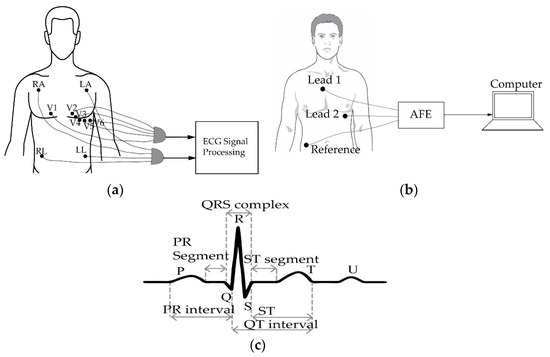
\includegraphics[height=7cm,width=12cm]{Images/chapter1/1-1.jpg}
\caption{(الف) سیستم الکتروکاردیوگرام بالینی؛ (ب) سیستم الکتروکاردیوگرام قابل حمل؛ (ج) نمایش سیگنال \lr{ECG}.\cite{kebe2020human}
}
\end{figure}
\end{center}
\vspace{2cm}



% ====================  اهداف و سوالات پژوهش  ====================

\section{اهداف و سوالات پژوهش}\label{sec1}



هدف اصلی این پژوهش، ارزیابی و تحلیل قابلیت‌های رادارهای \lr{FMCW (Frequency Modulated Continuous Wave)} در اندازه‌گیری ضربان قلب انسان است. این تحقیق به بررسی چگونگی استفاده از این رادارها در شرایط مختلف محیطی و چالش‌های فنی مربوط به کاربرد آنها در اندازه‌گیری ضربان قلب می‌پردازد. به‌طور کلی، اهداف این پژوهش به شرح زیر است:
\begin{enumerate}
    \item \textbf{تحلیل اصول عملکرد رادارهای \lr{FMCW}}: بررسی نحوه عملکرد و ویژگی‌های این نوع رادارها و شبیه‌سازی کاربرد آن‌ها در اندازه‌گیری ضربان قلب.
    \item \textbf{بررسی دقت اندازه‌گیری ضربان قلب با استفاده از رادارهای \lr{FMCW}}: ارزیابی دقت و قابلیت اطمینان اندازه‌گیری ضربان قلب در مقایسه با روش‌های سنتی مانند الکتروکاردیوگرام (\lr{ECG}).
    \item \textbf{بررسی اثرات مختلف محیطی بر عملکرد رادار}: تحلیل تأثیر عواملی مانند حرکت بدن، فاصله، موانع فیزیکی و شرایط محیطی بر دقت اندازه‌گیری ضربان قلب با رادارهای \lr{FMCW}.
    \item \textbf{طراحی سیستم اندازه‌گیری ضربان قلب با رادار \lr{FMCW}}: ارائه یک مدل یا الگوریتم برای بهبود دقت اندازه‌گیری ضربان قلب با استفاده از رادارهای \lr{FMCW} 
    \item \textbf{پیشنهاد کاربردهای پزشکی و بهداشتی رادارهای \lr{FMCW}}: بررسی استفاده از رادارهای \lr{FMCW} برای پایش و نظارت بر سلامت بیماران، به‌ویژه  پزشکی از راه دور.
\end{enumerate}


برای دستیابی به اهداف پژوهش، چندین سوال اصلی مطرح است که پاسخ به آنها می‌تواند به روشن شدن چالش‌ها و فرصت‌های استفاده از رادارهای \lr{FMCW} در اندازه‌گیری ضربان قلب کمک کند:
\begin{enumerate}
    \item چگونه می‌توان از رادارهای \lr{FMCW} برای اندازه‌گیری دقیق ضربان قلب انسان استفاده کرد؟
    \item آیا دقت اندازه‌گیری ضربان قلب با رادار \lr{FMCW} قابل مقایسه با روش‌های سنتی مانند \lr{ECG} است؟
    \item چه عواملی مانند حرکت بدن، فاصله، و موانع فیزیکی می‌توانند بر عملکرد رادار \lr{FMCW} در اندازه‌گیری ضربان قلب تأثیر بگذارند؟
    \item چه چالش‌ها و محدودیت‌هایی در استفاده از رادارهای \lr{FMCW} برای اندازه‌گیری ضربان قلب در شرایط مختلف محیطی وجود دارد؟
    \item چه تکنیک‌هایی می‌توانند دقت اندازه‌گیری ضربان قلب با استفاده از رادارهای \lr{FMCW} را در محیط‌های شلوغ یا پرتحرک بهبود بخشند؟
    \item چه مزایایی در استفاده از رادارهای \lr{FMCW} برای اندازه‌گیری ضربان قلب در مقایسه با روش‌های تهاجمی و تماس فیزیکی وجود دارد؟
    \item چه کاربردهایی برای استفاده از رادارهای \lr{FMCW} در نظارت بر سلامت بیماران و پایش از راه دور در پزشکی وجود دارد؟
\end{enumerate}

% ====================  اهمیت و نوآوری تحقیق ====================
\section{اهمیت و نوآوری تحقیق}\label{sec1}
\subsection{اهمیت تحقیق}\label{sec1}

با پیشرفت‌های روزافزون در تکنولوژی‌های ارتباطی و پردازشی، اندازه‌گیری ضربان قلب به عنوان یک پارامتر حیاتی در تشخیص وضعیت سلامت انسان، همواره در مرکز توجه محققان و پزشکان قرار داشته است. در این راستا، روش‌های سنتی اندازه‌گیری ضربان قلب که معمولاً به تجهیزات خاص یا تماس فیزیکی با بدن مانند الکتروکاردیوگرام (\lr{ECG}) یا پالس اکسیمتر وابسته هستند، می‌توانند برای بیماران دردناک باشند یا حتی در بعضی موارد عملی نباشند. به‌ویژه در محیط‌های بیمارستانی شلوغ یا در هنگام مراقبت‌های از راه دور، این روش‌ها ممکن است کارآیی و دقت کافی نداشته باشند.
با توجه به این محدودیت‌ها، استفاده از تکنولوژی‌های جدید مانند رادارهای \lr{FMCW} به عنوان یک راهکار دقیق برای اندازه‌گیری ضربان قلب، اهمیت ویژه‌ای پیدا کرده است. رادارهای \lr{FMCW} با استفاده از امواج رادیویی قادر به شبیه‌سازی حرکت‌های بسیار کوچک در بدن انسان، مانند تغییرات ناشی از ضربان قلب، هستند. این قابلیت‌ها باعث می‌شود که رادارهای \lr{FMCW} به ابزاری مؤثر در زمینه مراقبت‌های پزشکی از راه دور، پایش سلامت بیماران و حتی در محیط‌های پرتحرک تبدیل شوند.
این تحقیق می‌تواند با بررسی و ارزیابی کاربرد رادارهای \lr{FMCW} در اندازه‌گیری ضربان قلب، کمک شایانی به گسترش کاربرد این تکنولوژی در حوزه‌های پزشکی و بهداشت عمومی کند. با توجه به عدم نیاز به تماس فیزیکی و قابلیت اندازه‌گیری ضربان قلب در شرایط متنوع، این تحقیق می‌تواند زمینه‌ساز تحول در روش‌های نظارت بر سلامت انسان باشد.

\subsection{نوآوری تحقیق}\label{sec2}

نوآوری این تحقیق در استفاده از رادارهای \lr{FMCW}  برای اندازه‌گیری ضربان قلب به‌صورت غیرتماسی و در شرایط مختلف محیطی است. این نوآوری شامل جنبه‌های زیر می‌باشد:
\begin{enumerate}
    \item \textbf{استفاده از رادارهای \lr{FMCW} برای اندازه‌گیری ضربان قلب}: رادارهای \lr{FMCW} تا به امروز بیشتر در زمینه‌های نظامی، فضایی و صنعتی کاربرد داشته‌اند، اما این تحقیق اولین گام در استفاده از این رادارها برای اندازه‌گیری دقیق ضربان قلب انسان است. استفاده از این رادارها به‌عنوان ابزاری دقیق برای پایش سلامت، یک نوآوری در علوم پزشکی به‌شمار می‌رود.
    \item \textbf{اندازه‌گیری ضربان قلب در محیط‌های پرتحرک}: از آنجایی که رادارهای \lr{FMCW} قادر به اندازه‌گیری حرکت‌های بسیار کوچک در بدن هستند، این تحقیق به بررسی توانایی این رادارها در اندازه‌گیری ضربان قلب در شرایطی مانند حرکت بدن، فاصله، یا محیط‌های شلوغ و پرتحرک پرداخته است. این ویژگی می‌تواند تحولی در مراقبت‌های پزشکی از راه دور و نظارت بر وضعیت بیماران در هنگام فعالیت‌های روزمره باشد.
    \item \textbf{کاربرد رادارهای \lr{FMCW} در پایش سلامت از راه دور}: این تحقیق همچنین به بررسی کاربردهای رادارهای \lr{FMCW} در پایش ضربان قلب بیماران از راه دور پرداخته است. در این زمینه، رادارهای \lr{FMCW} می‌توانند به‌عنوان یک ابزار نظارتی بی‌دردسر و دقیق در مراکز درمانی و بیمارستان‌ها، بدون نیاز به تجهیزات اضافی یا تماس فیزیکی، عمل کنند.
    \item \textbf{توسعه الگوریتم‌های پردازش سیگنال برای بهبود دقت اندازه‌گیری}: یکی دیگر از جنبه‌های نوآورانه این تحقیق، طراحی و بهینه‌سازی الگوریتم‌های پردازش سیگنال برای تحلیل داده‌های رادار \lr{FMCW} به منظور افزایش دقت اندازه‌گیری ضربان قلب در شرایط مختلف محیطی است. این الگوریتم‌ها می‌توانند تغییرات کوچک در امواج راداری ناشی از ضربان قلب را از سایر سیگنال‌ها تفکیک کرده و دقت اندازه‌گیری را بهبود بخشند.
\end{enumerate}


% ==================== روش‌شناسی تحقیق   ====================
\section{روش‌شناسی تحقیق} % Corresponds to 1.4
\label{sec:methodology}

\subsection{مقدمه} % Corresponds to 1.4.1
\label{sec:methodology-intro}
روش‌شناسی تحقیق در این مطالعه، شامل طراحی و پیاده‌سازی یک سیستم اندازه‌گیری ضربان قلب مبتنی بر رادار \lr{FMCW} است. این تحقیق به‌منظور ارزیابی دقت، عملکرد و قابلیت‌های رادارهای \lr{FMCW} برای اندازه‌گیری ضربان قلب در شرایط مختلف محیطی و عملیاتی طراحی شده است. در این فصل، به‌تفصیل روش‌ها و مراحل مختلف تحقیق شامل طراحی سیستم، نحوه جمع‌آوری داده‌ها، تحلیل داده‌ها و ارزیابی عملکرد سیستم پرداخته خواهد شد.

\subsection{طراحی سیستم راداری \lr{FMCW}} % Corresponds to 1.4.2
\label{sec:fmcw-system-design}
در ابتدا، یک سیستم راداری \lr{FMCW} برای اندازه‌گیری ضربان قلب طراحی می‌شود. این سیستم شامل اجزای زیر است:
\begin{enumerate}
    \item \textbf{منبع سیگنال راداری}: یک سیگنال مدولاسیون فرکانسی پیوسته تولید می‌شود که فرکانس آن به‌طور پیوسته تغییر می‌کند.
    \item \textbf{آنتن راداری}: برای ارسال و دریافت سیگنال‌های رادیویی به‌کار می‌رود.
    \item \textbf{مدار پردازش سیگنال}: سیگنال‌های دریافتی از آنتن پردازش شده و تغییرات ناشی از ضربان قلب استخراج می‌شود.
    \item \textbf{سیستم تحلیل داده‌ها}: پس از پردازش سیگنال، الگوریتم‌های مختلف برای تحلیل و استخراج ضربان قلب از داده‌های راداری استفاده می‌شود.
\end{enumerate}

\subsection{جمع‌آوری داده‌ها} % Corresponds to 1.4.3
\label{sec:data-collection}
برای جمع‌آوری داده‌ها، آزمایش‌های مختلف با استفاده از رادار \lr{FMCW} در محیط‌های متفاوت طراحی می‌شود. داده‌ها از دو بخش اصلی استخراج می‌شوند:
\begin{itemize}
    \item **داده‌های راداری**: این داده‌ها از سیگنال‌های بازتاب‌شده از بدن انسان که تحت تأثیر ضربان قلب تغییر می‌کنند، به‌دست می‌آید.
    \item **داده‌های مرجع**: برای مقایسه دقت سیستم راداری، از روش‌های سنتی اندازه‌گیری ضربان قلب مانند الکتروکاردیوگرام (\lr{ECG}) یا پالس اکسیمتر به‌عنوان داده‌های مرجع استفاده می‌شود.
\end{itemize}
آزمایش‌ها در شرایط مختلف انجام خواهد شد، از جمله در حالت ایستاده، نشسته و در حال حرکت، تا قابلیت اندازه‌گیری ضربان قلب در شرایط عملیاتی متفاوت ارزیابی گردد.

\subsection{(این بخش را باید بازنویس کنم )تحلیل داده‌ها و پردازش سیگنال} % Corresponds to 1.4.4 - Note: Your numbering was '4.' but should be '1.4.4' as a subsection.
\label{sec:data-analysis-signal-processing}
برای استخراج ضربان قلب از سیگنال‌های راداری، نیاز به استفاده از تکنیک‌های پردازش سیگنال است. این مرحله شامل چندین مرحله مهم است:
\begin{itemize}
    \item **فیلتر کردن سیگنال‌ها**: سیگنال‌های راداری ممکن است حاوی نویزهایی باشند که باید فیلتر شوند. از فیلترهای دیجیتال برای حذف نویزهای اضافی و بهبود دقت اندازه‌گیری استفاده می‌شود.
    \item **تبدیل فوریه**: سیگنال‌های راداری برای استخراج فرکانس تغییرات ضربان قلب به تبدیل فوریه نیاز دارند. این تبدیل به ما کمک می‌کند تا فرکانس ضربان قلب را از سیگنال‌های راداری استخراج کنیم.
    \item **تحلیل زمان-فرکانس**: برای شبیه‌سازی دقیق‌تر رفتار ضربان قلب، از روش‌های زمان-فرکانس مانند تبدیل ویولت برای استخراج ویژگی‌های دقیق‌تر استفاده می‌شود.
\end{itemize}

\subsubsection{ارزیابی دقت و مقایسه با روش‌های سنتی} % This corresponds to 1.4.4.1 (as it's a sub-part of 1.4.4)
\label{sec2}
در این مرحله، دقت سیستم راداری \lr{FMCW} با استفاده از داده‌های مرجع مقایسه می‌شود. برای ارزیابی دقت اندازه‌گیری ضربان قلب، معیارهای زیر در نظر گرفته می‌شوند:
\begin{itemize}
    \item **خطای مطلق اندازه‌گیری (\lr{MAE})**: تفاوت بین ضربان قلب اندازه‌گیری شده توسط رادار \lr{FMCW} و داده‌های مرجع.
    \item **دقت اندازه‌گیری**: درصد انطباق اندازه‌گیری‌ها با داده‌های مرجع.
    \item **پایداری اندازه‌گیری**: ارزیابی اینکه آیا سیستم در شرایط مختلف محیطی، از جمله حرکت بدن یا تغییرات در فاصله، قادر به حفظ دقت خود است یا خیر.
\end{itemize}

\subsection{تحلیل نتایج و بررسی شرایط مختلف} % Corresponds to 1.4.5
\label{sec:results-analysis}
در این بخش، نتایج به‌دست‌آمده از آزمایش‌ها تجزیه و تحلیل می‌شود. نتایج عملکرد رادار \lr{FMCW} در شرایط مختلف مانند ایستاده، نشسته و در حال حرکت، به‌طور جامع بررسی می‌شود. همچنین تأثیر عواملی مانند فاصله، موانع فیزیکی و شرایط محیطی (مانند حضور افراد دیگر یا نویز رادیویی) بر دقت اندازه‌گیری ضربان قلب بررسی خواهد شد.

\subsection{بهینه‌سازی سیستم} % Corresponds to 1.4.6
\label{sec:system-optimization}
در نهایت، بر اساس نتایج به‌دست‌آمده، بهینه‌سازی‌هایی برای سیستم پیشنهاد می‌شود. این بهینه‌سازی‌ها می‌تواند شامل بهبود الگوریتم‌های پردازش سیگنال، بهبود حساسیت راداری، و کاهش اثرات محیطی بر دقت اندازه‌گیری باشد.




% ==================== مروری بر کارهای مرتبط  ====================
\section{مروری بر کارهای مرتبط} % Corresponds to 1.5
\label{sec:related-work}

\subsection{رادارهای پزشکی و کاربردهای آن‌ها} % Corresponds to 1.5.1
\label{sec:medical-radars}

در سال‌های اخیر، فناوری رادار به‌ویژه در کاربردهای پزشکی مورد توجه ویژه‌ای قرار گرفته است.\cite{li2013review} برخلاف کاربردهای سنتی رادار در صنایع نظامی و خودرو، امروزه رادارها در زمینه‌هایی مانند پایش علائم حیاتی (ضربان قلب و نرخ تنفس)، تشخیص سقوط بیماران، شناسایی حرکت‌های غیرارادی بدن، و پایش بیماران در اتاق مراقبت‌های ویژه مورد استفاده قرار می‌گیرند. این سیستم‌ها، برای بیماران با شرایط خاص، نوزادان و سالمندان مزیت چشم‌گیری دارند.
برخی پژوهش‌ها به بررسی عملکرد رادارهای میلی‌متری برای شناسایی علائم حیاتی در اتاق‌های بیمارستانی یا حتی در محیط خانگی پرداخته‌اند. برای مثال، از رادارهای \lr{Doppler} برای اندازه‌گیری نرخ تنفس استفاده شده و مشخص شده که این رادارها قادر به تشخیص تغییرات کوچک در قفسه سینه فرد هستند. همچنین رادارهای \lr{FMCW} و \lr{UWB} در این زمینه در حال رشد چشمگیری‌اند، چرا که قابلیت تفکیک مکانی و حساسیت بالاتری دارند.

\subsection{اندازه‌گیری ضربان قلب با رادار: روش‌های \lr{CW}، \lr{FMCW}، و \lr{UWB}} % Corresponds to 1.5.2
\label{sec:heart-rate-radar-methods}

اندازه‌گیری ضربان قلب با رادار، با استفاده از روش‌های مختلفی امکان‌پذیر است که هرکدام مزایا و محدودیت‌های خاص خود را دارند:
\begin{itemize}
    \item \textbf{رادار موج پیوسته (\lr{CW})}: در این روش، رادار سیگنال سینوسی با فرکانس ثابت ارسال می‌کند و تغییرات فاز سیگنال بازتاب‌شده را برای تشخیص حرکت‌های ظریف بدن (مثل ضربان قلب) تحلیل می‌کند. این روش ساده است، اما توان تفکیک مکانی ندارد و در محیط‌های با چند هدف یا نویز بالا عملکرد خوبی ندارد.
    \item \textbf{رادار \lr{FMCW (Frequency Modulated Continuous Wave)}}: این روش با استفاده از مدولاسیون خطی فرکانس، امکان تخمین فاصله و همچنین استخراج اطلاعات حرکت ظریف را فراهم می‌آورد. رادارهای \lr{FMCW} با دقت بالا می‌توانند ضربان قلب را در فاصله‌های مختلف و بدون تماس ثبت کنند. پژوهش‌هایی مانند \lr{Li et al. (2018)} و \lr{Wang et al. (2020)} به نتایج موفقی در این زمینه دست یافته‌اند و قابلیت استفاده از \lr{FMCW} را در شرایط متحرک یا پرنویز اثبات کرده‌اند.\cite{yue2020non}
    \item \textbf{رادار باند فوق‌گسترده (\lr{UWB})}: این نوع رادار با ارسال پالس‌های کوتاه و پهن‌باند، قادر به اندازه‌گیری دقیق موقعیت و حرکت است. مزیت آن توانایی بالا در تفکیک مکانی و کاهش اثرات تداخل می‌باشد. در عین حال، به دلیل الزامات تنظیمی و پیچیدگی سخت‌افزار، کاربرد آن در عمل ممکن است محدود شود.
\end{itemize}

\subsection{خلأها و چالش‌های موجود} % Corresponds to 1.5.3
\label{sec:gaps-challenges}

با وجود پیشرفت‌های قابل‌توجه در اندازه‌گیری ضربان قلب با استفاده از رادار، همچنان چالش‌ها و خلأهایی در این حوزه باقی مانده است:
\begin{enumerate}
    \item \textbf{نویز و تداخل حرکتی}: یکی از چالش‌های اصلی، تداخل ناشی از حرکت‌های بزرگ بدن یا حضور اشیاء متحرک در محیط است که می‌تواند بر روی سیگنال ضربان قلب اثر بگذارد و دقت اندازه‌گیری را کاهش دهد.
    \item \textbf{تفکیک ضربان قلب از نرخ تنفس}: در بسیاری از موارد، سیگنال‌های ناشی از تنفس قوی‌تر از سیگنال ضربان قلب هستند و استخراج دقیق ضربان قلب نیازمند فیلترینگ دقیق یا استفاده از الگوریتم‌های پردازش سیگنال پیشرفته است.\cite{adib2015smart}
    \item \textbf{نبود مدل استاندارد برای مقایسه عملکرد}: بیشتر تحقیقات از روش‌های خاص خود برای اندازه‌گیری و ارزیابی استفاده کرده‌اند و فقدان یک استاندارد یا دیتاست عمومی باعث دشواری در مقایسه دقیق میان روش‌ها می‌شود.
    \item \textbf{پیاده‌سازی در شرایط واقعی}: بسیاری از مطالعات در محیط‌های کنترل‌شده آزمایشگاهی انجام شده‌اند. پیاده‌سازی موفق در محیط‌های واقعی (مانند اتاق بیمار، خودرو یا منزل) نیازمند بهینه‌سازی طراحی آنتن، مدارات پردازش و حذف نویز محیطی است.
    \item \textbf{نیاز به الگوریتم‌های هوشمند پردازش سیگنال}: برای استخراج دقیق ضربان قلب از داده‌های راداری، به‌ویژه در حضور نویز و حرکات اضافی، نیاز به الگوریتم‌های پیشرفته یادگیری ماشین، پردازش سیگنال تطبیقی و تحلیل چند متغیره احساس می‌شود.
\end{enumerate}



\vspace{2cm}
\begin{center}
\begin{figure}[!h]
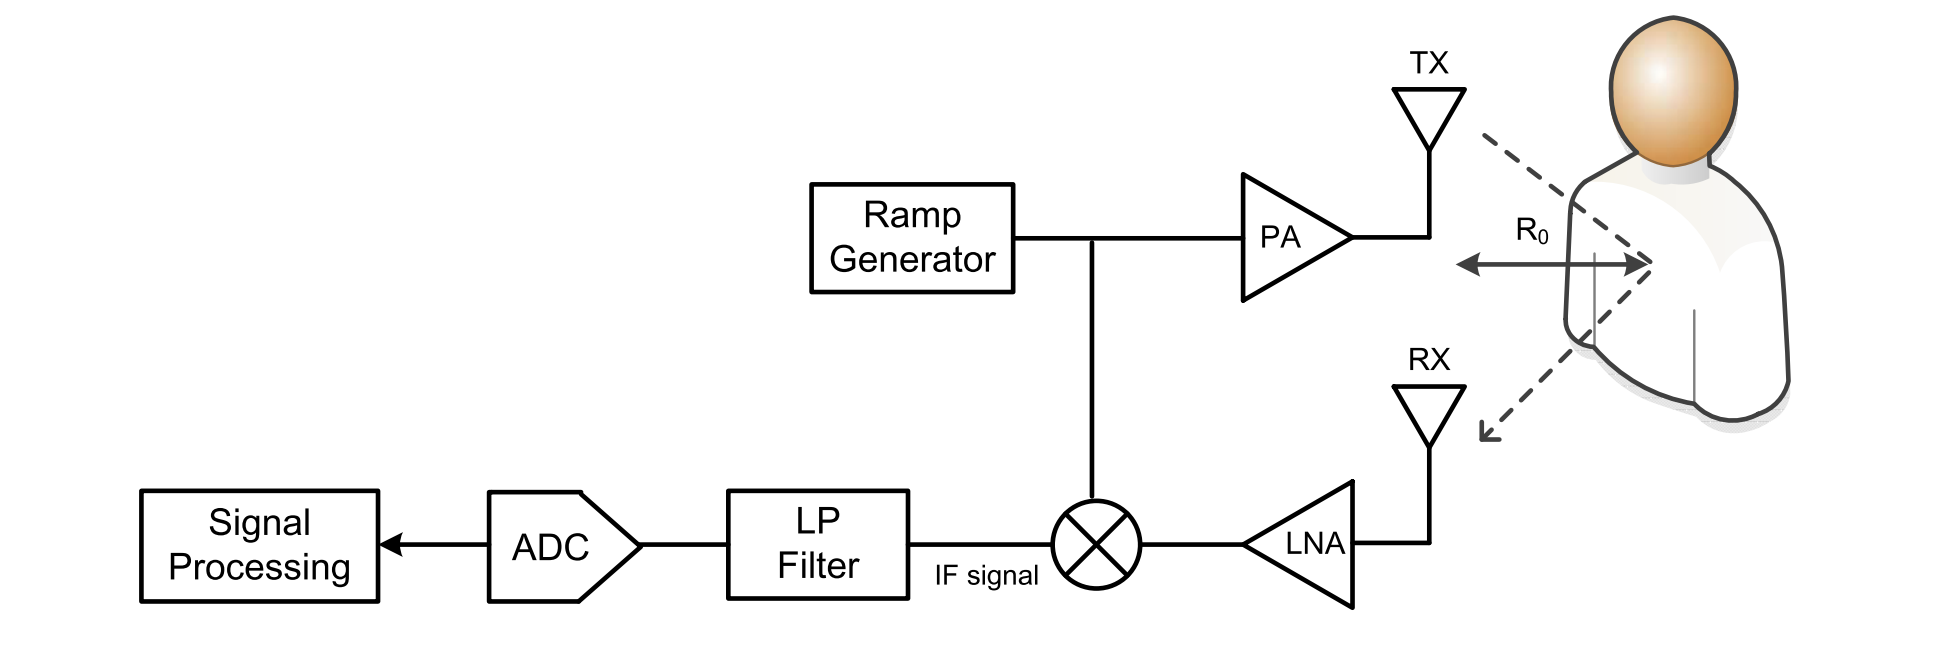
\includegraphics[height=4cm,width=12cm]{Images/chapter1/1-2.png}
\caption{بلاک دیاگرام رادار \lr{fmcw}.\cite{adib2015smart}
}
\end{figure}
\end{center}
\vspace{2cm}



\chapter{مبانی نظری رادار \lr{FMCW} و فیزیولوژی ضربان قلب}
\label{ch:fmcw-physiology}

% ====================  مقدمه  ====================

\section{مقدمه}
در این فصل به دو محور اصلی پرداخته می‌شود:

بررسی فیزیولوژی ضربان قلب و الگوی حرکتی با تأکید بر ویژگی‌های سیگنال‌های حرکتی (\lr{micro-motions}) قفسه سینه که ناشی از تپش‌های قلب هستند؛

مبانی نظری رادار \lr{FMCW (Frequency-Modulated Continuous-Wave)} و پارامترهای کلیدی طراحی آن تشریح شده و روش‌های پردازش پیشرفته برای جداسازی و اندازه‌گیری دقیق ضربان قلب به‌صورت غیرتماسی ارائه می‌شوند. در بخش اول، با مروری بر مکانیسم انقباض و انبساط میوکارد و انتشار موج پرفیوژن، نشان داده می‌شود که چگونه تغییرات بسیار کوچک موقعیت سطح قفسه سینه (در حد میلی‌متر یا کمتر) حامل اطلاعات حیاتی ضربان و نرخ متغیر قلب است. این تبیین فیزیولوژیک، مبنای انتخاب پارامترهای راداری مناسب را فراهم می‌آورد.

در بخش دوم، اصول کار رادارهای \lr{FMCW} با معرفی سیگنال‌های \lr{Chirp} و رابطه فرکانس \lr{Beat} برای اندازه‌گیری فاصله و سرعت توضیح داده خواهد شد
. سپس پارامترهای پهنای باند (\lr{B})، مدت زمان چرخه (\lr{Tp}) و نسبت سیگنال به نویز (\lr{SNR}) مورد بررسی قرار می‌گیرند که هر یک تأثیر مستقیمی بر دقت فاصله‌سنجی و تشخیص کوچک‌ترین حرکات دارند.

در ادامه، روش‌های متنوع پردازش سیگنال با هدف بهبود جداسازی ضربان قلب از نویز و حرکات مزاحم بدن مرور می‌شوند:
\begin{itemize}
  \item ارتقای تفکیک‌پذیری هم‌زمان فاصله و سرعت در رادارهای قابل پیکربندی
  \item مقایسه کارایی رادارهای داپلر و \lr{FMCW} در پایش علائم حیاتی غیرتماسی
  \item به‌کارگیری نمونه‌برداری انتخابی برای گسترش دامنه سرعت قابل تشخیص
  \item استفاده از رادار میلی‌متری جهت پایش هم‌زمان چند سوژه و کاهش نویز با کمک الگوریتم تجزیه مقادیر منفرد (\lr{SVD})
  \item تحلیل تغییرات درون‌فردی سیگنال‌های سیزموکاردیوگرام
  \item ارائه چارچوب‌های چندهدفه برای استخراج و پایش تغییرات ضربان قلب
\end{itemize}

این ساختار فصل، خواننده را از مبانی فیزیولوژیک تا روش‌های نوین 
پردازش سیگنال راداری هدایت می‌کند و زمینه را برای ارائه روش تحقیق و نتایج تجربی در فصل‌های بعدی فراهم می‌آورد.



% ====================  اصول کار رادار  ====================
\section{اصول کار رادار \lr{FMCW}}\label{sec:fmcw-principles}


\subsection{سیگنال چیپ (\lr{Chirp}) و پهنای باند} % Subsection 2.1.1
\label{sec:chirp-bandwidth}

رادارهای \lr{FMCW (Frequency-Modulated Continuous Wave)} از نوع خاصی از امواج رادیویی استفاده می‌کنند که فرکانس آن‌ها به‌صورت خطی در بازه‌ای از زمان تغییر می‌کند. به این سیگنال‌ها، «چیپ» (\lr{Chirp}) گفته می‌شود. در یک چرخه از عملکرد رادار، سیگنال فرستاده‌شده از نوع خطی صعودی است که در آن فرکانس از یک مقدار آغازین \lr{$f_0$} تا مقدار \lr{$f_0 + B$} در مدت زمان \lr{$T$} افزایش می‌یابد.





\vspace{2cm}
\begin{center}
\begin{figure}[!h]
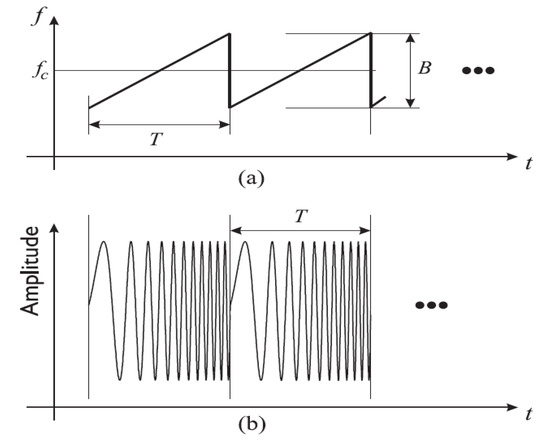
\includegraphics[height=10cm,width=12cm]{Images/chapter2/2-1.jpg}
\caption{(\lr{a}) تغییر فرکانس در طول زمان، (\lr{b}) سیگنال‌های \lr{chirp} لحظه‌ای.
\cite{kebe2020human}
}
\end{figure}
\end{center}
\vspace{2cm}

ویژگی کلیدی این نوع سیگنال در اندازه‌گیری فاصله، قابلیت نمایش موقعیت فاصله‌ای اهداف با استفاده از اختلاف فرکانسی بین سیگنال ارسال‌شده و سیگنال بازتابی است. هنگامی که سیگنال بازتابی از یک هدف با تأخیر زمانی دریافت می‌شود، اختلاف فرکانس بین سیگنال دریافتی و ارسال‌شده (که به آن \lr{beat frequency} گفته می‌شود) مستقیماً با فاصله هدف مرتبط است.


فرکانس \lr{beat} با رابطه زیر تعیین می‌شود:
\begin{equation}
f_b = \frac{2BR}{cT}
\label{eq:beat_frequency}
\end{equation}
\addequation{اختلاف فرکانس بین سیگنال دریافتی و ارسال‌شده}

که در آن:
\begin{itemize}
    \item \lr{$B$}: پهنای باند سیگنال چیپ
    \item \lr{$R$}: فاصله تا هدف
    \item \lr{$c$}: سرعت نور
    \item \lr{$T$}: مدت‌زمان سیگنال
\end{itemize}

 در کاربردهای زیستی مانند پایش ضربان قلب، حرکت‌های بسیار ظریف سطح قفسه سینه (در حد میلی‌متر یا کمتر) باعث ایجاد تغییرات فرکانسی بسیار کوچک در سیگنال برگشتی می‌شود، که با تحلیل دقیق این \lr{beat frequency} می‌توان علائم حیاتی نظیر ضربان قلب را استخراج کرد.
\cite{munoz2018doppler}

در مقاله \cite{neemat2019reconfigurable}، تمرکز بر افزایش قدرت تفکیک (\lr{resolution}) در محور فاصله است. طبق یافته‌های این مقاله، پهنای باند سیگنال چیپ مستقیماً بر توان تفکیک فاصله اثرگذار است.تفکیک فاصله‌ای \lr{$\Delta R$} به‌صورت زیر تعریف می‌شود:
\begin{equation}
\Delta R = \frac{c}{2B}
\label{eq:range_resolution}
\end{equation}
\addequation{رابطه‌ی تفکیک فاصله‌ای در رادار \lr{FMCW}}

بنابراین، افزایش پهنای باند باعث بهبود توانایی سیستم در تمایز اهداف نزدیک به هم می‌شود. در کاربردهای پزشکی مانند اندازه‌گیری ضربان قلب، که در آن سیگنال‌های بسیار ضعیف از حرکت‌های سطحی بدن ثبت می‌شود، این افزایش تفکیک می‌تواند به تفکیک بهتر نویز محیطی از سیگنال واقعی ضربان قلب منجر شود.
همچنین به معرفی پردازش دامنه داپلر قابل پیکربندی (\cite{neemat2019reconfigurable}) پرداخته است که با تغییر معماری فریم‌های چیپ، امکان جداسازی بهتر سیگنال‌های مربوط به تنفس و ضربان قلب فراهم می‌شود. این موضوع در شرایطی که حرکت‌های دیگر بدن وجود دارند (مانند تکان‌های سر یا دست)، اهمیت دوچندان پیدا می‌کند.
در جمع‌بندی این بخش، می‌توان گفت که استفاده از سیگنال‌های چیپ با پهنای باند بالا، نه‌تنها دقت فاصله‌سنجی را در رادارهای \lr{FMCW} افزایش می‌دهد، بلکه با بهره‌گیری از روش‌هایی مانند \lr{Range-Doppler} قابل پیکربندی، تفکیک و تحلیل دقیق‌تری از علائم حیاتی فراهم می‌آورد.

%=================================================================================================


\subsection{آشکارسازی فاصله و سرعت} 
\label{sec:range-velocity-detection}

رادارهای \lr{FMCW (Frequency-Modulated Continuous Wave)} از سیگنال‌های خطی چیپ (\lr{Chirp}) برای اندازه‌گیری فاصله و سرعت استفاده می‌کنند. یکی از ویژگی‌های کلیدی رادارهای \lr{FMCW} توانایی آشکارسازی دقیق فاصله (\lr{Range}) و سرعت (\lr{Doppler Velocity}) اهداف مختلف است. برای دستیابی به این قابلیت، رادار \lr{FMCW} از اصول پیچیده‌ای برای پردازش سیگنال‌ها استفاده می‌کند که در مقایسه با رادارهای \lr{CW (Continuous Wave)} و \lr{Pulse}، مزایای بیشتری را در دقت اندازه‌گیری فراهم می‌آورد.

\subsubsection{آشکارسازی فاصله} % Corresponds to 2.1.2.1
\label{sec:range-detection}

در رادار \lr{FMCW}، فاصله تا هدف از طریق تحلیل فرکانس \lr{beat} که نتیجه اختلاف فرکانس بین سیگنال ارسالی و بازتابی است، محاسبه می‌شود. این اختلاف فرکانسی به‌طور مستقیم با فاصله‌ی هدف مرتبط است و طبق رابطه‌ی زیر تعیین می‌شود:
\begin{equation}
f_b = \frac{2B \cdot R}{cT}
\label{eq:beat_frequency}
\end{equation}
\addequation{رابطه‌ی فرکانس \lr{beat} برحسب فاصله‌ی هدف}

که در آن:
\begin{itemize}
    \item \lr{$f_b$}: فرکانس \lr{beat}،
    \item \lr{$B$}: پهنای باند سیگنال چیپ،
    \item \lr{$R$}: فاصله تا هدف،
    \item \lr{$c$}: سرعت نور،
    \item \lr{$T$}: مدت‌زمان چرخه‌ی سیگنال.
\end{itemize}

\vspace{2cm}
\begin{center}
\begin{figure}[!h]
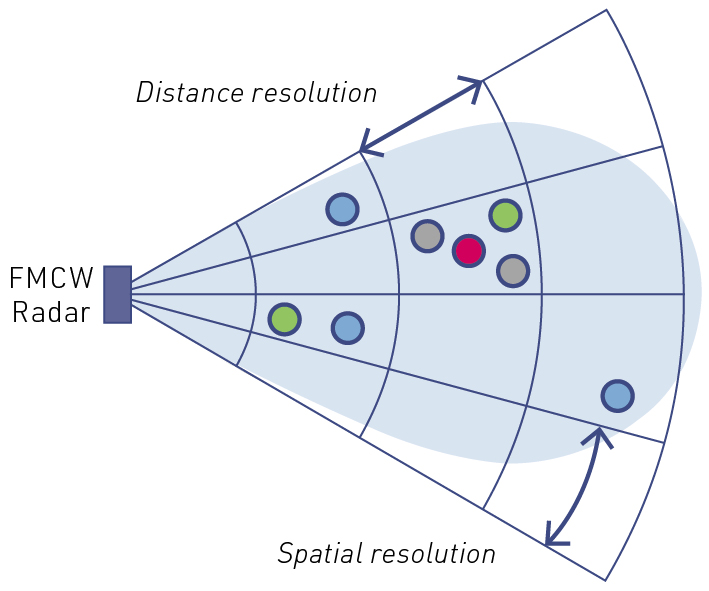
\includegraphics[height=10cm,width=12cm]{Images/chapter2/2-2.jpg}
\caption{تشخیص و تفکیک اهداف مختلف در میدان دید رادار \lr{fmcw}
\cite{rfbeam2024}
}
\end{figure}
\end{center}
\vspace{2cm}

برای دقیق‌تر کردن اندازه‌گیری فاصله در رادارهای \lr{FMCW}، افزایش پهنای باند سیگنال چیپ اهمیت ویژه‌ای دارد. همان‌طور که در مقاله \cite{neemat2019reconfigurable} اشاره شده است، با افزایش پهنای باند \lr{$B$}، دقت تفکیک فاصله بهبود می‌یابد، چرا که تفکیک فاصله \lr{$\Delta R$} به‌طور معکوس با پهنای باند نسبت دارد:
\begin{equation}
\Delta R = \frac{c}{2B}
\label{eq:range_resolution}
\end{equation}
\addequation{رابطه‌ی تفکیک فاصله‌ای برحسب پهنای باند}

این ویژگی، به‌ویژه در کاربردهایی مانند اندازه‌گیری ضربان قلب، که تغییرات فازی کوچکی به‌دلیل حرکت قفسه سینه به وجود می‌آید، بسیار حیاتی است.

\subsubsection{آشکارسازی سرعت} % Corresponds to 2.1.2.2
\label{sec:velocity-detection}

در رادار \lr{FMCW}، سرعت اهداف به کمک اثر داپلر (\lr{Doppler Effect}) و تحلیل فرکانس داپلر استخراج می‌شود.سیگنال‌های بازتابی از اهداف متحرک موجب تغییر در فرکانس آن‌ها می‌شوند که این تغییر به‌عنوان تغییر فرکانس داپلر در سیگنال دریافت‌شده ظاهر می‌شود. فرکانس داپلر با سرعت هدف مرتبط است \cite{kwak2024adjusting} و به‌صورت زیر محاسبه می‌شود:
\begin{equation}
f_d = \frac{2v}{\lambda}
\label{eq:doppler_frequency}
\end{equation}
\addequation{رابطه‌ی فرکانس داپلر برحسب سرعت هدف و طول‌موج}

که در آن:
\begin{itemize}
    \item \lr{$f_d$}: فرکانس داپلر،
    \item \lr{$v$}: سرعت نسبی هدف نسبت به رادار،
    \item \lr{$\lambda$}: طول‌موج سیگنال رادار.
\end{itemize}

یکی از چالش‌ها در سیستم‌های رادار \lr{FMCW}، محدودیت دامنه سرعت قابل تشخیص است. سرعت‌های بسیار پایین یا سرعت‌های بالا ممکن است باعث شود که سیگنال داپلر تغییرات نامشخص یا حتی معکوس داشته باشد، که در نتیجه منجر به از دست رفتن سیگنال یا کاهش دقت در تشخیص سرعت می‌شود.
برای حل این مشکل، مقاله \cite{kwak2024adjusting} به تکنیک‌هایی برای نمونه‌برداری انتخابی (\lr{Selective Sampling}) اشاره کرده است که با تنظیم فواصل نمونه‌برداری، می‌توان دامنه سرعت قابل تشخیص را افزایش داد. به این معنا که می‌توان سیستم رادار را طوری تنظیم کرد که دامنه‌ای گسترده‌تر از سرعت‌ها را با دقت بیشتری اندازه‌گیری کند، بدون اینکه از کیفیت اندازه‌گیری فاصله کاسته شود.


\subsubsection{پیشرفت‌ها در پردازش دامنه داپلر و فاصله} % Corresponds to 2.1.2.3
\label{sec:advanced-range-doppler-processing}

یکی دیگر از چالش‌ها در سیستم‌های رادار \lr{FMCW}، نیاز به پردازش دقیق و بهینه داده‌ها در دامنه داپلر و فاصله است. مقاله \cite{neemat2019reconfigurable}  توضیح می‌دهد که استفاده از پردازش دامنه داپلر قابل پیکربندی می‌تواند به بهبود تفکیک سرعت و فاصله در سیستم‌های راداری \lr{FMCW} کمک کند. این روش با تنظیم پارامترهای سیستم در هر فریم، به رادار اجازه می‌دهد که دامنه‌های وسیع‌تری از سرعت و فاصله را پردازش کند و در عین حال از تداخل‌های نامطلوب جلوگیری کند.
پردازش دامنه داپلر به سیستم‌های راداری اجازه می‌دهد تا علاوه بر اندازه‌گیری فاصله، سرعت حرکت اهداف مانند حرکت قفسه سینه در هنگام ضربان قلب را به‌طور دقیق شبیه‌سازی و اندازه‌گیری کنند. این قابلیت برای کاربردهای پزشکی مانند پایش ضربان قلب در شرایط مختلف حرکت یا تغییر موقعیت بدن، به‌ویژه در مواقعی که حرکت‌های بدن موجب اختلال در سیگنال می‌شود، بسیار مفید است.


%=================================================================================================




% ====================  پارامترهای کلیدی در طراحی  ====================
\section{پارامترهای کلیدی در طراحی \lr{FMCW} (\lr{B}, \lr{$T_p$}, \lr{SNR} و ...)}\label{sec:fmcw-key-parameters} % Corresponds to 2.2


در سیستم‌های رادار \lr{FMCW}، طراحی بهینه و انتخاب مناسب پارامترهای مختلف تأثیر بسزایی در دقت اندازه‌گیری، عملکرد، و قابلیت تشخیص اهداف دارد. در این بخش، به بررسی پارامترهای کلیدی در طراحی سیستم‌های \lr{FMCW} پرداخته خواهد شد که به‌ویژه در کاربردهای پزشکی مانند اندازه‌گیری ضربان قلب اهمیت زیادی دارند. این پارامترها شامل پهنای باند (\lr{B})، مدت زمان چرخه (\lr{$T_p$})، نسبت سیگنال به نویز (\lr{SNR}) و برخی دیگر از فاکتورهای مهم در طراحی سیستم راداری هستند.

\subsection{پهنای باند (\lr{B})} % Corresponds to 2.2.1
\label{sec:bandwidth}

پهنای باند \lr{$B$} یکی از مهم‌ترین پارامترها در طراحی سیستم‌های راداری \lr{FMCW} است. افزایش پهنای باند منجر به دقت بالاتر در اندازه‌گیری فاصله و تفکیک بهتر اهداف می‌شود. طبق مقاله \cite{islam2020non}، با افزایش پهنای باند، سیستم قادر به تمایز بهتر میان اهداف نزدیک به هم خواهد بود که این ویژگی در اندازه‌گیری‌های پزشکی بسیار حائز اهمیت است، به‌ویژه برای تمایز ضربان قلب از دیگر سیگنال‌های جسمی.
رابطه‌ی پهنای باند با تفکیک فاصله به‌صورت زیر بیان می‌شود:
\begin{equation}
\Delta R = \frac{c}{2B}
\label{eq:range_resolution_bandwidth}
\end{equation}
\addequation{رابطه‌ی میان پهنای باند و تفکیک فاصله‌ای}

که در آن \lr{$\Delta R$} تفکیک فاصله و \lr{$c$} سرعت نور است. این رابطه نشان می‌دهد که با افزایش \lr{$B$}، تفکیک فاصله بهبود می‌یابد و دقت اندازه‌گیری افزایش می‌یابد. در اندازه‌گیری ضربان قلب، این ویژگی باعث می‌شود که سیستم بتواند تغییرات جزئی در حرکت بدن که ناشی از ضربان قلب است، با دقت بیشتری شبیه‌سازی کند.

\subsection{مدت زمان چرخه (\lr{$T_p$})} % Corresponds to 2.2.2
\label{sec:chirp-duration}

مدت زمان چرخه \lr{$T_p$} که به آن مدت زمان مدولاسیون نیز گفته می‌شود، تأثیر زیادی بر عملکرد رادارهای \lr{FMCW} دارد. مدت زمان مدولاسیون، مدت زمانی است که سیگنال فرکانس خطی تغییر می‌کند. طبق مقاله \cite{lv2024millimeter}، افزایش مدت زمان \lr{$T_p$} موجب افزایش دقت در شبیه‌سازی تغییرات ضربان قلب می‌شود، زیرا طولانی‌تر شدن چرخه سیگنال امکان تحلیل دقیق‌تر تغییرات سیگنال‌های برگشتی را فراهم می‌آورد.
با توجه به این مقاله، افزایش مدت زمان چرخه می‌تواند باعث بهبود توانایی سیستم در تمایز نویز از سیگنال اصلی ضربان قلب شود. همچنین، انتخاب مدت زمان مناسب برای مدولاسیون سیگنال، ارتباط مستقیمی با دقت اندازه‌گیری سرعت و تفکیک داپلر دارد.

\subsection{نسبت سیگنال به نویز (\lr{SNR})} % Corresponds to 2.2.3
\label{sec:snr}

یکی از چالش‌های اصلی در سیستم‌های راداری \lr{FMCW}، حفظ نسبت سیگنال به نویز (\lr{SNR}) مناسب است. \lr{SNR} یکی از عوامل مهمی است که کیفیت داده‌های دریافتی و دقت اندازه‌گیری را تحت تأثیر قرار می‌دهد. سیستم‌های راداری با \lr{SNR} پایین قادر به تشخیص دقیق تغییرات کوچک در سیگنال‌های برگشتی نخواهند بود، که این مشکل در اندازه‌گیری ضربان قلب در شرایط مختلف محیطی، به‌ویژه در محیط‌های پر نویز مانند بیمارستان‌ها یا محیط‌های شلوغ، به‌وضوح مشاهده می‌شود.
مقاله \cite{islam2020non} به این موضوع پرداخته و اشاره می‌کند که برای پایش علائم حیاتی به‌ویژه ضربان قلب، لازم است که \lr{SNR} به‌گونه‌ای تنظیم شود که سیگنال‌های مرتبط با ضربان قلب به وضوح از نویزهای دیگر تمایز یابند. یکی از روش‌های پیشنهادی برای بهبود \lr{SNR}، استفاده از تکنیک‌های پردازش سیگنال پیشرفته و فیلترینگ هوشمند است.
بهبود \lr{SNR} معمولاً با استفاده از افزایش پهنای باند (\lr{B})، بهبود الگوریتم‌های پردازش سیگنال و افزایش قدرت سیگنال‌های ارسالی امکان‌پذیر است. این کار می‌تواند باعث کاهش اثرات نویز محیطی بر روی داده‌های دریافتی شود.

\subsection{سایر پارامترهای طراحی} % Corresponds to 2.2.4
\label{sec:other-design-parameters}

علاوه بر پارامترهای فوق، در طراحی سیستم‌های \lr{FMCW} برای اندازه‌گیری ضربان قلب، دیگر پارامترها نیز باید در نظر گرفته شوند. برای مثال:
\begin{itemize}
    \item \textbf{آنتن راداری}: طراحی آنتن با قابلیت پوشش‌دهی مناسب برای اندازه‌گیری دقیق اهداف با فاصله‌های مختلف، یکی از ارکان کلیدی طراحی سیستم رادار \lr{FMCW} است.
    \item \textbf{توان سیگنال ارسالی}: میزان توان سیگنال ارسال‌شده می‌تواند بر کیفیت داده‌های دریافتی و حساسیت سیستم تأثیرگذار باشد.
    \item \textbf{پردازش سیگنال تطبیقی}: استفاده از الگوریتم‌های تطبیقی برای فیلتر کردن نویز و شبیه‌سازی دقیق‌تر ضربان قلب می‌تواند به افزایش دقت سیستم کمک کند.
\end{itemize}




% ====================  نتیجه‌گیری  ====================
\section{نتیجه‌گیری}
در پایان این فصل روشن شد که رادارهای \lr{FMCW} با بهره‌گیری از سیگنال‌های \lr{Chirp} و تحلیل \lr{Range–Doppler} می‌توانند حرکات بسیار کوچک ناشی از ضربان قلب را با دقت میلی‌متری تشخیص دهند. افزایش پهنای باند و طول چرخه مدولاسیون (\lr{Tp}) به‌طور مستقیم دقت فاصله‌سنجی را بهبود می‌بخشد، در حالی که حفظ نسبت سیگنال به نویز (\lr{SNR}) بالا برای جداسازی ضربان از نویز محیطی و حرکات تصادفی بدن حیاتی است.

پیشرفت‌های اخیر در پردازش دوبعدی \lr{Range–Doppler} \cite{neemat2019reconfigurable} و نمونه‌برداری انتخابی \cite{kwak2024adjusting} دامنه سرعت قابل اندازه‌گیری را گسترش داده و امکان پایش ضربان قلب در شرایط محیطی و سوژه‌های متحرک بیشتر را فراهم کرده‌اند. روش‌های کاهش نویز مبتنی بر تجزیه مقادیر منفرد (\lr{SVD}) \cite{lv2024millimeter} و بررسی اثرات تغییرات درون‌فردی سیگنال‌های \lr{seismocardiogram} \cite{demirsoy2024investigating} نیز دقت تخمین نرخ ضربان و \lr{HRV} را ارتقاء داده‌اند.

علاوه بر این، کاربرد رادار میلی‌متری در پایش چندسوژه‌ای \cite{islam2020non} و تشخیص چندهدفه \lr{HRV} \cite{xu2024health} نشان داده که با طراحی مناسب آنتن و الگوریتم‌های هوشمند، می‌توان به راه‌حل‌های غیرتماسی دقیق و کارآمد برای کاربردهای پزشکی دست یافت. با این وجود، چالش‌هایی نظیر تداخل متقابل میان سوژه‌ها، کاهش \lr{SNR} در محیط‌های شلوغ و پیچیدگی محاسباتی پردازش \lr{Range–Doppler} همچنان باقی است.

\begin{figure}[ht]
    \centering
    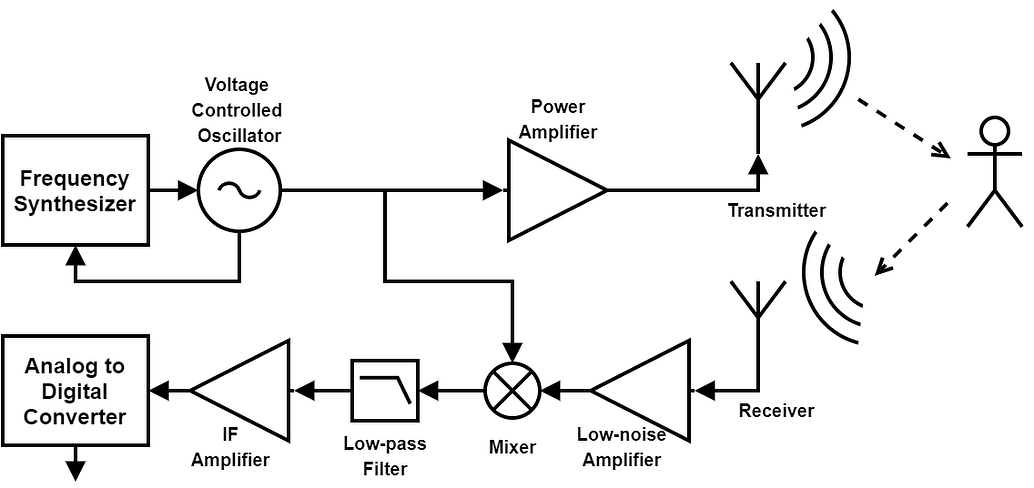
\includegraphics[width=0.7\linewidth]{Images/chapter2/2-3.png}
    \caption{اندازه‌گیری علائم حیاتی با استفاده از رادار \lr{mmWave FMCW} \cite{digikey_fmcw}.}
    \label{fig:fmcw_vitals}
\end{figure}

\vspace{5cm}

فصل بعدی با تکیه بر این مبانی، روش پیشنهادی پژوهش را تشریح خواهد کرد، که در آن با طراحی آزمایش و انتخاب پارامترهای بهینه رادار، تلاش می‌شود محدودیت‌های مطرح‌شده برطرف گردد و کارایی سیستم در پایش ضربان قلب واقعی ارزیابی شود.





\chapter{طراحی سیستم و پیاده‌سازی}

% ====================  مقدمه  ====================
\section{مقدمه}\label{sec:intro-cap3}

% در سال‌های اخیر، نظارت مداوم بر علائم حیاتی انسان (ضربان قلب و نرخ تنفس) به‌عنوان ابزاری کلیدی در تشخیص به‌موقع حوادث حاد و پیش‌بینی زودهنگام وخامت شرایط بالینی مطرح شده است. روش‌های مرسوم مبتنی بر تماس، نظیر \lr{ECG} و \lr{PPG}، اگرچه دقت بالایی ارائه می‌دهند، اما به دلیل نیاز به تماس مستقیم با پوست، در شرایطی نظیر سوختگی، زخم‌های پوستی یا پاندمی‌ها می‌توانند کارآمدی و ایمنی کافی را نداشته باشند.

% در این راستا، رادارهای غیرتماسی مبتنی بر امواج \lr{میلی‌متری‌موج (mmWave)} به دلیل نفوذپذیری مطلوب در بافت‌های سطحی و مقاومت بالا در برابر تغییرات نوری و دمای محیط، به‌عنوان جایگزینی مناسب شناخته شده‌اند. میان انواع مختلف معماری‌های راداری، \lr{FMCW} به‌واسطه مدولاسیون فرکانس خطی، قابلیت تفکیک اهداف چندگانه و همزمان سنجش فاصله و حرکت را فراهم می‌آورد، که در پیاده‌سازی‌های غیرتماسی علائم حیاتی مزایای چشمگیری دارد.

% متون مروری اخیر نشان می‌دهند که تحقیقات متعددی به مقایسه و تحلیل معماری‌های \lr{CW}، \lr{FMCW} و \lr{UWB} پرداخته‌اند. برای نمونه، \lr{Liebetruth} و همکاران (2024) مروری سیستماتیک بر اندازه‌گیری ضربان قلب و تنفس با رادار ارائه داده‌اند و بر نقش متمایز مدولاسیون فرکانس در حذف اختلال‌های محیطی تأکید کرده‌اند. همچنین، \lr{Bin Obadi} و همکاران (2021) در یک مرور جدید، علاوه بر بررسی معماری‌های مختلف، به پیاده‌سازی نرم‌افزاری روی \lr{FPGA} و چالش‌های آن پرداخته‌اند.

% با این حال، اگرچه مطالعات بسیاری بر روی تخمین ضربان قلب و نرخ تنفس متمرکز شده‌اند، تحلیل جامعی از تأثیر پارامترهای فرکانس حامل و پهنای باند بر دقت اندازه‌گیری علائم حیاتی و نیز بررسی کامل جنبه‌های ایمنی و انطباق با استانداردهای پزشکی تا پیش از این کم‌تر انجام شده است. این شکاف پژوهشی انگیزه‌ای قوی برای ارائه یک بررسی متمرکز بر کاربرد رادارهای \lr{FMCW} در پزشکی ایجاد می‌کند.

% در ادامه، ابتدا مبانی فیزیکی و اصول کار رادارهای \lr{FMCW} همراه با بررسی تاریخچه کاربرد آن‌ها در پایش حیاتی بدن مرور خواهد شد. سپس تحولات کلیدی در الگوریتم‌های پردازش سیگنال و پروژه‌های عملی پیاده‌سازی سخت‌افزاری مورد بحث قرار می‌گیرند، تا زمینه‌ای روشن برای طراحی سیستم پیشنهادی این پایان‌نامه فراهم آید.


پایش مداوم علائم حیاتی به‌صورت غیرتماسی، چه در بخش‌های مراقبت ویژه و چه در پایش خانگی بیماران مزمن، نیازمند فناوری‌ای است که هم دقت بالای الکترودهای تماسی را داشته باشد و هم زحمت کمتری برای بیمار ایجاد کند. در میان سه معماری متداول راداری—\lr{CW}، \lr{UWB} و \lr{FMCW}—معماری \lr{FMCW} با ترکیب مدولاسیون خطی فرکانس و پردازش \lr{Beat Signal}، امکان اندازه‌گیری همزمان فاصله و ریزحرکت سطح قفسهٔ سینه را با پیچیدگی سخت‌افزاری قابل قبولی فراهم می‌کند؛ در نتیجه، خطاهای نقطهٔ کور \lr{CW} و محدودیت برد \lr{UWB} تا حد زیادی برطرف می‌شوند.

این فصل ابتدا نشان می‌دهد که چگونه پهنای باند مدولاسیون بر تفکیک‌پذیری فاصله اثر می‌گذارد:

\begin{equation}
\Delta R \approx \frac{c}{2B}
\label{eq:range_resolution}
\end{equation}
\addequation{اثر پهنای باند مدولاسیون بر تفکیک‌پذیری فاصله در سامانه‌های راداری}

و چرا بازه‌ی \lr{1–4 GHz} برای فواصل پزشکی \lr{0.5} تا \lr{3} متر کافی است. سپس به این نکته پرداخته می‌شود که افزایش فرکانس حامل در طیف میلی‌متری، طول موج را کوتاه و حساسیت فاز را افزایش می‌دهد؛ نتایج آزمایش روی رادارهای \lr{60 GHz} و \lr{120 GHz} نشان داده است که دقت اندازه‌گیری ضربان قلب در حدود $\pm 3.1$ \lr{bpm} و خطای تنفس کمتر از \lr{2 brpm} باقی می‌ماند، در حالی که سیستم \lr{24 GHz} به‌دلیل پروفایل نویز بالا کارایی ضعیف‌تری از خود نشان می‌دهد.

بر این مبنا، سخت‌افزار ارائه‌شده در این فصل بر پایه‌ی چیپ \lr{TI IWR1642} با آرایه‌ی مجتمع \lr{MIMO}، توان مصرفی کمتر از \lr{30 mW} و ساختار برد ارزیابی مدولار طراحی شده است؛ انتخابی که امکان جداسازی چند بیمار، اندازه‌ی کوچک، و سازگاری با باتری‌های پوشیدنی را فراهم می‌کند.

در ادامه، زنجیره‌ی پردازش شامل استخراج \lr{Beat Signal}، کالیبراسیون \lr{DC}، بازکردن فاز، فیلتر باندگذر تنفس و ضربان، سرکوب حرکات، و استفاده از الگوریتم \lr{Health-VMD} برای تخمین \lr{HRV} شرح داده می‌شود.

در نهایت، ملاحظات ایمنی، محدودیت توان تابشی، و مسیر اخذ مجوزهای بالینی تکمیل‌کننده‌ی چرخه‌ی طراحی سیستم به‌شمار می‌آیند.


% ====================  مقایسه رادارها  ====================
\section{مقایسه معماری‌های راداری (\lr{FMCW، CW، UWB})}
\label{sec:radar-architecture-comparison}

در این بخش سه معماری اصلی راداری که در سامانه‌های غیرتماسی پایش علائم حیاتی کاربرد دارند \lr{CW (Continuous Wave)}، \lr{FMCW (Frequency-Modulated Continuous Wave)} و \lr{UWB (Ultra-Wideband)}از نظر اصول کاری، پیچیدگی پیاده‌سازی و عملکرد مقایسه می‌شوند.

\subsection{اصول کار معماری‌ها}
\label{sec:principles}

در رادارهای \lr{CW}، سیگنال با فرکانس ثابت و تابش مداوم فرستاده می‌شود و تغییر فاز سیگنال بازتابی به‌عنوان نشانگر حرکت سطح قفسه سینه تحلیل می‌گردد. این سادگی سخت‌افزاری، هزینه و توان مصرفی پایین را فراهم می‌کند؛ اما نقاط کور عمده آن عدم توان تعیین فاصله دقیق و حساسیت بالا به نویزهای چندمسیره است.
\cite{frazao2024radar}

در معماری \lr{FMCW}، فرکانس حامل به‌صورت خطی روی زمان مدوله می‌شود و با تطبیق سیگنال ارسالی و دریافتی (\lr{Beat Signal}) می‌توان هم فاصله و هم سرعت حرکت را استخراج کرد. پهنای باند مدولاسیون رابطه ­مستقیمی با رزولوشن فاصله‌ای دارد:

\begin{equation}
\Delta R = \frac{c}{2B}
\label{eq:range_resolution_bandwidth}
\end{equation}
\addequation{رابطه‌ی میان پهنای باند و تفکیک فاصله‌ای}

و به‌دلیل مدولاسیون فرکانس، این معماری در برابر نویز های محیطی مقاوم‌تر است.
\cite{frazao2024radar}

معماری \lr{UWB} با ارسال پالس‌های کوتاه و گسترده‌پهنای‌باند، تأخیر انتشار موج را برای تخمین فاصله می‌سنجد. گرچه دقت فاصله‌یابی آن بالاست، سخت‌افزار پیچیده و نیاز به پردازش‌های سنگین سیگنال از موانع عمده کاربردهای بالینی آن است.
\cite{paterniani2023radar}

\subsection{مزایا و محدودیت‌ها}
\label{sec:advantages-limitations}

\begin{itemize}
    \item \textbf{\lr{CW}}: کم‌هزینه و ساده؛ مناسب کاربردهای اولیه اما فاقد جداسازی اهداف و مقاومتی اندک در برابر \lr{Multipath Clutter}.
    \item \textbf{\lr{FMCW}}: توازن مطلوب بین سخت‌افزار و قابلیت‌های فاصله‌یابی و تفکیک چندهدفه. پهنای باند بزرگ‌تر، رزولوشن بالاتر و حذف اغتشاشات ناشی از بازتاب‌های ناخواسته را فراهم می‌کند.
    \item \textbf{\lr{UWB}}: دقت بسیار بالا در اندازه‌گیری تأخیر انتشار و امکان نفوذ از موانع جدار نازک؛ اما طراحی آنتن و پردازش دیجیتال پیچیده، هزینه و مصرف انرژی را افزایش می‌دهد.
\end{itemize}


\begin{figure}[ht]
    \centering
    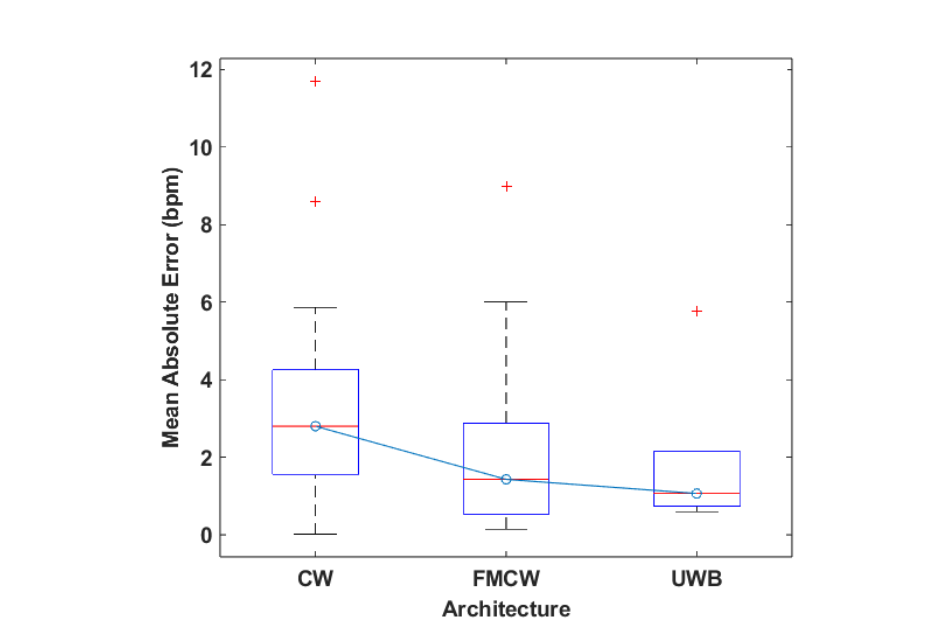
\includegraphics[width=0.7\linewidth]{Images/chapter3/3-2.png}
    \caption{ نمودار جعبه‌ای مقادیر \lr{MAE} برای هر معماری.\cite{frazao2024radar}.}
    \label{fig:fmcw_vitals}
\end{figure}

\subsection{عملکرد آزمایشگاهی و خطاهای اندازه‌گیری}
\label{sec:experimental-performance}

بررسی داده‌های منتشرشده در ۵۶ مطالعه‌ی اندازه‌گیری ضربان قلب نشان می‌دهد که معماری \lr{FMCW} کمترین میانه‌ی خطای مطلق (\lr{MAE}) را دارد، در حالی که \lr{CW} بیشترین میانه‌ی خطا را به خود اختصاص داده است. اگرچه \lr{UWB} در مقایسه‌ی تعداد مطالعات کمتر است، دامنه خطای این معماری کوچک‌تر بوده اما برای تأیید برتری آن نیاز به مطالعات بیشتر است.

به‌طور خاص، در شکل جعبه‌ای (\lr{Boxplot}) مقایسه خطاها، معماری \lr{CW} دارای بالاترین میانه و دامنه‌ی گسترده‌تری از خطا است، در حالی که \lr{FMCW} توزیع خطا فشرده‌تر و \lr{UWB} پایین‌ترین مقادیر حداکثر خطا را نشان می‌دهد. این نتایج گویای برتری معماری \lr{FMCW} در سنجش غیرتماسی ضربان قلب به‌واسطه‌ی مقاومت آن در برابر نویز و تداخل محیطی است.

% \subsection{نتیجه‌گیری موقت}
% \label{sec:interim-conclusion}

% با توجه به مقایسه‌ی مزایا، معایب و داده‌های تجربی، معماری \lr{FMCW} گزینه‌ی اول برای سامانه‌های پزشکی غیرتماسی محسوب می‌شود. \lr{CW} علیرغم سادگی، به‌دلیل عدم امکان تفکیک فاصله و حساسیت بالا به نویز به‌عنوان جایگزین دوم مطرح است و \lr{UWB}، هرچند پتانسیل دقت بالایی دارد، به‌علت پیچیدگی سخت‌افزاری و کمبود مطالعات بالینی گسترده، هنوز در مرحله آزمایشگاهی قرار دارد. در فصل‌های بعدی، بسته به نیازمندی‌های بالینی و محدودیت‌های سخت‌افزاری، انتخاب معماری مناسب برای طراحی سامانه‌ی پایان‌نامه تشریح خواهد شد.


% ====================  انتخاب فرکانس و پهنای باند مناسب  ====================
\section{انتخاب فرکانس و پهنای باند مناسب}
\label{sec:frequency-band-selection}

\subsection{نقش پهنای باند در رزولوشن فاصله‌ای و برد آشکار}
پهناي باند مدولاسیون (\lr{B}) در رادارهای \lr{FMCW} تعیین‌کننده‌ی رزولوشن فاصله‌ای است. به‌طور دقیق، رزولوشن فاصله‌ای با رابطه
\begin{equation}
\Delta R \approx \frac{c}{2B}
\end{equation}
محاسبه می‌شود؛ به‌عبارت دیگر، افزایش \lr{B} موجب کوچک‌تر شدن $\Delta R$ و توانایی تفکیک اهداف نزدیک‌تر می‌شود. از سوی دیگر، بزرگ‌تر شدن پهنای باند می‌تواند برد آشکار ($R_\text{\lr{max}}$) را کاهش دهد، مگر آنکه تعداد نمونه‌ها در هر چیپ (\lr{N}) یا نرخ نمونه‌برداری افزایش یابد، چرا که
\begin{equation}
R_\text{\lr{max}} = \frac{c\,N}{4B}\,.
\end{equation}

در کاربردهای پزشکی غیرتماسی که فاصله‌ی بیمار تا رادار معمولاً در محدوده‌ی \lr{0.5–3 } متر قرار دارد، پهنای باند \lr{1–4 GHz} معمولاً کفاف رزولوشن  و برد آشکار کافی را می‌دهد.

\subsection{تأثیر فرکانس حامل بر حساسیت فاز و عمق نفوذ}
انتخاب فرکانس حامل ($f_c$) در طیف \lr{mmWave} (\lr{30–300 GHz}) به دلیل تأثیر مستقیم بر حساسیت فاز به تغییرات  کوچک‌تر از میلی‌متر و عمق نفوذ الکترومغناطیسی دارای اهمیت است. با افزایش $f_c$ و کاهش طول موج ($\lambda = c/f_c$)، تغییرات کوچک دیواره قفسه‌ی سینه به تغییر فاز بزرگ‌تر تبدیل می‌شوند که استخراج ضربان قلب را دقیق‌تر می‌کند. از سویی دیگر، نفوذپذیری پوست با افزایش فرکانس کاهش می‌یابد (برای مثال عمق نفوذ از \lr{2.7 mm} در \lr{10 GHz} به \lr{0.5 mm} در \lr{60 GHz} می‌رسد)، اما بازتاب از سطح پوست قوی‌تر شده و تأثیر پوشش‌های پارچه‌ای ناچیز می‌گردد.

در مطالعه‌ی مقایسه‌ای بر روی سه رادار کم‌مصرف \lr{FMCW} با فرکانس‌های \lr{24}، \lr{60} و \lr{120 GHz}، نتایج زیر گزارش شده است:
\begin{itemize}
  \item نرخ تنفس (\lr{RR}) با خطای مطلق میانگین (\lr{MAE}) کمتر از \lr{2 brpm} برای هر سه سیستم؛
  \item ضربان قلب (\lr{HR}) با \lr{MAE} برابر $1.8 \pm 3.1$ \lr{bpm} برای سیستم \lr{60 GHz} و $3.2 \pm 5.3$ \lr{bpm} برای سیستم \lr{120 GHz}؛
  \item اما سیستم \lr{24 GHz} به‌دلیل پروفایل نویز بالا، \lr{MAE} حدود \lr{9.0 bpm} داشت.
\end{itemize}

این داده‌ها نشان می‌دهد که انتخاب فرکانس حامل در بازه‌ی \lr{60–120 GHz} می‌تواند به‌طور قابل‌توجهی دقت استخراج علائم حیاتی را افزایش دهد، به‌ویژه زمانی که محدودیت‌های سخت‌افزاری و مصرف توان نیز باید در نظر گرفته شوند.

\subsection{موازن‌سازی در کاربردهای عملی}
اگرچه فرکانس‌های بالاتر (بیش از \lr{60 GHz}) دقت بالاتری ارائه می‌دهند، پیاده‌سازی آنتن و مصرف توان آن‌ها چالش‌برانگیز است. رادارهای کم‌مصرف با توان ده‌ها میلی‌وات و پهنای باند چندگیگاهرتز، نقطه‌ی توازنی میان دقت بالا و قابلیت پیاده‌سازی پوشیدنی فراهم می‌کنند. برای بسیاری از کاربردهای بالینی نظیر نظارت بر بیماران در تخت با پوشش لباس یا ملحفه استفاده از فرکانس‌های میانی (\lr{60–80 GHz}) توصیه می‌شود، چرا که علاوه بر حساسیت فاز مناسب، عمق نفوذ کافی و هزینه‌ی معقول سخت‌افزاری را نیز تأمین می‌کنند.


% ====================  معماری سخت‌افزاری  ====================
\section{طراحی سخت‌افزار و معماری سیستم}

در این فصل، جزئیات پیاده‌سازی سخت‌افزار سامانه مبتنی بر رادار \lr{FMCW} جهت اندازه‌گیری غیرتماسی علائم حیاتی تشریح می‌شود. ابتدا انتخاب چیپ‌ست راداری و پیکربندی آن بررسی می‌شود، سپس چگونگی ساختاربندی ماژول‌ها و ادغام آن‌ها در یک برد ارزیابی به همراه مشخصات آنتن و مصرف توان بیان می‌گردد. در نهایت، معماری \lr{MIMO} و مزایای آن در جداسازی چندشخص مورد بحث قرار می‌گیرد.

\subsection{انتخاب چیپ‌ست رادار و پیکربندی اولیه}

برای پیاده‌سازی رادار \lr{FMCW}، دو رویکرد اصلی مشاهده شده است:

\begin{itemize}
  \item چیپ‌های کم‌مصرف \lr{BGT} از شرکت \lr{Infineon} در فرکانس‌های ۲۴، ۶۰ و ۱۲۰ گیگاهرتز؛
  \item چیپ \lr{IWR1642} از شرکت \lr{Texas Instruments} در باند ۷۷–۸۱ گیگاهرتز.
\end{itemize}
در مجموعه آزمایشات اولیه، سه رادار \lr{BGT24}، \lr{BGT60} و \lr{BGT120} با بهره‌گیری از بردهای ارزیابی ماژولار استفاده شدند. هر کدام از این سیستم‌ها مصرف توانی در بازه‌ی ۸ تا ۲۶ میلی‌وات دارند و توان خروجی آن‌ها در حدود \lr{5 dBm} تنظیم شده است. تمامی تجهیزات روی یک پنل آکریلیکی نصب شده و برای کنترل زاویه و فاصله به سه‌پایه مجهز شده‌اند.

چیپ \lr{IWR1642} با باند فرکانسی \lr{77–81 GHz} و پهنای باند \lr{4 GHz}، به دلیل پشتیبانی داخلی از آرایه \lr{MIMO} و پردازش دیجیتال مجتمع، در طراحی سامانه نهایی این پایان‌نامه به‌عنوان پلتفرم اصلی انتخاب شده است. این چیپ ضمن فراهم آوردن امکان جداسازی زاویه‌ای، مصرف توان کمتر از \lr{30 mW} و نرخ نمونه‌برداری تا \lr{2 MHz} را پشتیبانی می‌کند.

\subsection{برد ارزیابی و ساختار مدولار}
\label{sec:eval-board-structure}

برای مقایسه عملکرد بین سیستم‌ها و سهولت تنظیم پارامترها، هر رادار روی یک \textbf{برد ارزیابی ماژولار} نصب شد که دارای:

\begin{itemize}
  \item درگاه‌های پیکربندی دیجیتال (\lr{SPI/I\textsuperscript{2}C}) برای تنظیم فرکانس شروع ($f_\text{start}$)، پهنای باند ($B$) و نرخ چیپ؛
  \item مبدل \lr{ADC} با نرخ نمونه‌برداری \lr{2 MHz}؛
  \item خروجی \lr{USB/Serial} برای انتقال داده‌های \lr{IF} به رایانه جهت پردازش؛
  \item رابط آنتن خارجی یا بسته (\lr{Antenna-in-Package}) مطابق با فرکانس کاری؛
\end{itemize}

این بردها امکان تغییر سریع \textbf{پارامترهای چیپ} مانند شیب چیپ را فراهم می‌کنند:

\begin{equation}
S = \frac{B}{T_c}
\label{eq:chirp_slope}
\end{equation}
\addequation{رابطه شیب فرکانسی (\lr{Chirp Slope}) بر حسب پهنای باند و مدت زمان هر چیپ}

و همچنین تعداد چیپ‌ها در هر بازه زمانی (\lr{Chirp Density}) قابل تنظیم است.

\subsection{مشخصات آنتن و میدان دید}
\label{sec:antenna-fov}

رادارهای \lr{BGT60} و \lr{BGT120} از \textbf{آنتن داخل بسته} با بهره‌ی \lr{3.5 dBi} و نیم‌توان عرض پرتو $65^\circ$ در صفحه \lr{E} و $45^\circ$ در صفحه \lr{H} بهره می‌برند. رادار \lr{BGT24} دارای \textbf{آنتن خارجی} با مشخصات مشابه در فرکانس \lr{24 GHz} است. انتخاب پهنای باند \lr{2–10 GHz} برای \lr{BGT}های مختلف، به‌ترتیب موجب رزولوشن فاصله‌ای \lr{7.5}، \lr{3} و \lr{1.5} سانتی‌متر شد.

چیپ \lr{IWR1642} نیز از آنتن‌‌های مجتمع \lr{MIMO} (شامل ۳ فرستنده و ۴ گیرنده) برخوردار است که امکان تعیین زاویه ورود (\lr{Angle of Arrival}) و جداسازی چندشخصه را فراهم می‌سازد. با استفاده از ترکیب \lr{Beamforming} و روش‌های \lr{TDM-Orthogonalization}، آرایه مجازی ۱۲ کانالی قابل دستیابی است که وضوح زاویه‌ای به‌صورت زیر خواهد بود:

\begin{itemize}
  \item $\approx 16.6^\circ$ در افق (سمت-به-سمت)
  \item $\approx 45^\circ$ در ارتفاع (پایین-به-بالا)
\end{itemize}

\subsection{مدیریت مصرف توان}
\label{sec:power-management}

با توجه به کاربردهای پوشیدنی و همراه پزشکی، \textbf{مصرف توان} یکی از معیارهای حیاتی است. در پیکربندی پایه با نرخ چیپ \lr{100 Hz}، مصرف هر چیپ در حدود \lr{8 mW} برآورد شد که با فعال‌ساز...


% ====================  نرم‌افزار پردازش اولیه  ====================
\section{پردازش سیگنال و الگوریتم‌های استخراج نرخ ضربان قلب}
\label{sec:signal-processing-hr-estimation}

در این بخش، زنجیره‌ی پردازش سیگنال از نمونه‌برداری تا تخمین نرخ ضربان قلب (\lr{HR}) و استخراج ضرباهنگ قلب برای تحلیل \lr{HRV} شرح داده می‌شود. فرایند شامل مراحل زیر است:


\begin{figure}[ht]
    \centering
    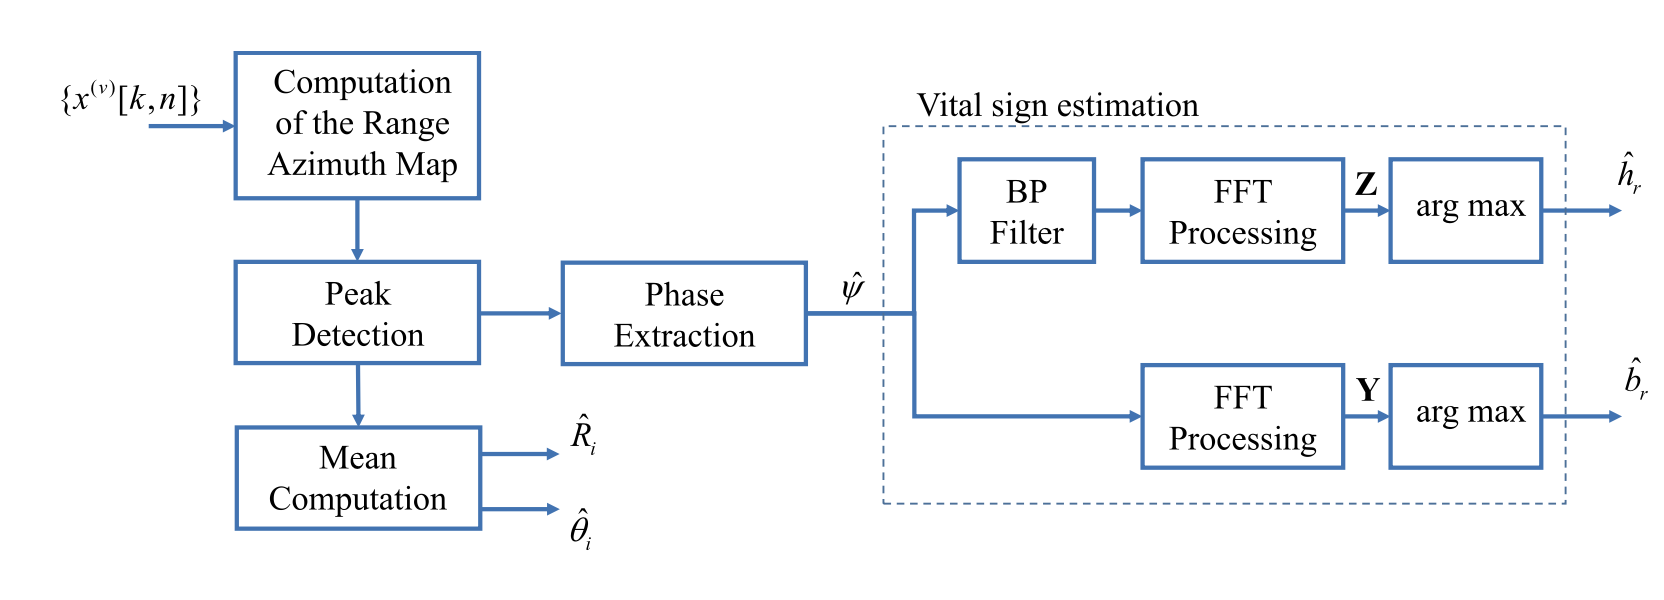
\includegraphics[width=0.7\linewidth]{Images/chapter3/3-3.png}
    \caption{
   نمایش پردازش سیگنال علائم حیاتی \lr{(HR و BR)} چندین نفر با استفاده از یک رادار \lr{MIMO} با موقعیت مکانی مشترک.
    \cite{paterniani2023radar}.}
    \label{fig:fmcw_vitals}
\end{figure}


\subsection{استخراج سیگنال میانی (\lr{Beat Signal}) و کالیبراسیون \lr{DC}}
\label{sec:beat-signal-dc-calibration}

پس از دریافت داده‌های \lr{IF} از مبدل آنالوگ‌به‌دیجیتال، یک \lr{FFT} مختصر (\lr{Slow-Time FFT}) روی هر چیپ انجام می‌شود تا فرکانس مناسب (\lr{bin}) مربوط به بازتاب از قفسه‌ی سینه انتخاب گردد. سپس سیگنال‌های \lr{I/Q} متناظر با آن \lr{bin} برای مراحل بعدی استخراج می‌شود.

از آنجا که خطاهای ساختاری ناشی از عدم تقارن \lr{I/Q} و \lr{DC Offset} می‌تواند موجب انحراف در فاز استخراجی شود، ابتدا با روش \lr{Least-Squares Circle Fitting} مؤلفه‌های \lr{DC} مجزای \lr{I} و \lr{Q} برآورد و حذف می‌شوند. با این کار، شکل موج فازِ استخراج‌شده به بازتاب واقعی سیگنال ضربان قلب نزدیک‌تر می‌گردد.


\subsection{استخراج فاز و آشفتگی‌زدایی (\lr{Phase Unwrapping})}
\label{sec:phase-unwrapping}

برای به‌دست آوردن فاز پیوسته‌ی حرکت قفسه‌ی سینه، از تابع آرکتانژانت دو متغیره استفاده می‌شود:

\begin{equation}
\phi[n] = \operatorname{atan2}(Q[n],\, I[n])
\label{eq:phase_extraction}
\end{equation}
\addequation{استخراج فاز از مؤلفه‌های \lr{I} و \lr{Q} با تابع آرکتانژانت دوارگشتی}

که خروجی در بازه $-\pi$ تا $\pi$ قرار دارد. سپس برای حذف جهش‌های ناخواسته بزرگ‌تر از $\pi$، الگوریتم \lr{Unwrapping} اجرا می‌شود. برای مواردی که جابجایی دیواره بیش از نیم طول موج باشد و \lr{Unwrapping} ساده خطا دهد، می‌توان از الگوریتم \lr{DACM (Differencing and Augmented Cross-Multiplication)} بهره برد.

\subsection{تقویت اجزاء ضربان قلب و حذف درفت فاز}
\label{sec:phase-detrend}

در سیگنال \lr{Unwrapped Phase}، مؤلفه‌های تنفسی با بازه‌ی فرکانسی بین 0.1 تا 0.5~\lr{Hz} معمولاً غالب‌تر از مؤلفه‌های ضربان قلب در بازه‌ی 0.8 تا 2.0~\lr{Hz} هستند. برای تقویت مؤلفه‌های ضربان، ابتدا تفاضل مرکزی فاز (بین نمونه‌های جلو و عقب) محاسبه می‌شود تا شیب‌های لحظه‌ای برجسته شوند:

\begin{equation}
\Delta \phi[n] = \phi[n+1] - \phi[n-1]
\label{eq:phase_diff}
\end{equation}
\addequation{محاسبه تفاضل مرکزی برای حذف روند و تقویت مولفه‌های پرنوسان مانند ضربان قلب}

در مواردی که مقدار تفاضل از آستانه‌ای بیش از حد بزرگ یا کوچک‌تر از منفی آستانه باشد، نمونه‌ها با درون‌یابی خطی اصلاح می‌شوند تا ناهمواری‌های ضربه‌ای (\lr{Impulse Noise}) برطرف گردد.

\subsection{فیلترینگ ناظر بر جداسازی بلوک‌های تنفس و ضربان}
\label{sec:bandpass-filtering}

پس از تفاضل فاز، دو فیلتر \lr{Bandpass IIR} مجزا اعمال می‌شود:

\begin{itemize}
  \item \lr{فیلتر دومرحله‌ای}: برای تفکیک مؤلفه‌های تنفسی در بازه‌ی فرکانسی \lr{0.1–0.5 Hz}
  \item \lr{فیلتر چهارمرحله‌ای}: برای جداسازی ضربان قلب در بازه‌ی \lr{0.8–2.0 Hz}
\end{itemize}

این ساختار به شکل بلادرنگ روی سیگنال اعمال و خروجی هر فیلتر برای مراحل بعدی نگهداری می‌شود.

\subsection{حذف اعوجاج ناشی از حرکت و کنترل بهره}
\label{sec:motion-artifacts}

برای مقابله با تداخل ناشی از حرکت‌های بزرگ بدن (\lr{Motion Corruption})، انرژی هر بخش یک‌ثانیه‌ای سیگنال ضربان قلب محاسبه می‌شود و با آستانه‌ای مقایسه می‌گردد:

\begin{equation}
E = \sum_{n=1}^{N} x^2[n]
\label{eq:energy}
\end{equation}
\addequation{محاسبه انرژی سیگنال در یک بازه زمانی به‌منظور شناسایی حرکت‌های ناخواسته}

در صورت عبور از آستانه، سیگنال مقیاس شده یا حذف می‌شود تا از ورود نویزهای حرکتی به تخمین جلوگیری گردد.

\subsection{ شناسایی پیک طیفی برای تخمین ضربان قلب}
\label{sec:peak-counting}

برای استخراج \lr{HR}، یک \lr{FFT} روی بخش‌های سالم خروجی فیلتر ضربان اجرا شده و قله‌ی طیفی متناظر با فرکانس قلب شناسایی می‌شود. تعداد پیک‌های متوالی در بازه‌ی زمانی مشخص، معادل نرخ ضربان قلب بر حسب \lr{bpm} است.

\subsection{تحلیل زمان فرکانس (\lr{STFT})}
\label{sec:stft}

به‌منظور ردیابی تغییرات لحظه‌ای ضربان و جداسازی بهتر هارمونیک‌های تنفس، از روش \lr{Short-Time Fourier Transform (STFT)} استفاده می‌شود. در هر پنجره‌ی زمانی، انرژی ترکیبی سیگنال به‌صورت زیر محاسبه می‌گردد:

\begin{equation}
E[n] = |x[n]|^2 + |y[n]|^2
\label{eq:stft_energy}
\end{equation}
\addequation{محاسبه انرژی در تحلیل \lr{STFT} برای تشخیص بازتاب‌های قوی از سطح بدن}

نقاط با بیشترین انرژی، بازتاب‌های ضربان قلب تلقی شده و تحلیل ادامه می‌یابد.

\subsection{الگوریتم \lr{Health-VMD} برای استخراج دقیق \lr{HRV}}
\label{sec:health-vmd}

برای تخمین \lr{HRV} نیاز به تشخیص دقیق هر ضربان (\lr{IBI}) است. در مقاله‌ی \lr{Health-Radar}، روش \lr{Variational Mode Decomposition (VMD)} با پارامترهای بهینه‌سازی‌شده توسط الگوریتم \lr{GOA (Grasshopper Optimization Algorithm)} پیشنهاد شده است. تابع هدف پیشنهادی:

\begin{equation}
\mathrm{PME} = \alpha \cdot H_{\mathrm{PE}} + \beta \cdot I_{\mathrm{MI}} + \gamma \cdot L_{\mathrm{Loss}}
\label{eq:pme_objective}
\end{equation}
\addequation{تابع هدف ترکیبی برای \lr{VMD} شامل آنتروپی جایگشتی، اطلاعات متقابل و نرخ اتلاف انرژی}


این روش تضمین می‌کند که هارمونیک‌های تنفس وارد مدهای ضربان نشوند. خروجی این الگوریتم، تخمین دقیق پارامترهایی نظیر \lr{SDNN} و \lr{RMSSD} است، با دقتی برابر:

\begin{equation}
\mathrm{RMSE} \approx 4.1\ \mathrm{ms}
\label{eq:rmse_sdnn}
\end{equation}
\addequation{خطای میانگین مربعی در تخمین \lr{SDNN} توسط الگوریتم \lr{Health-VMD}}

\subsection*{خلاصه‌ی نتایج}
\label{sec:summary}

با ترکیب مراحل فوق کالیبراسیون \lr{DC}، استخراج و \lr{Unwrapping} فاز، تفاضل و فیلترینگ \lr{IIR}، حذف آرتیفکت‌های حرکتی، \lr{STFT} و \lr{Health-VMD} دقت تخمین \lr{HR} به‌صورت زیر گزارش شده است:

\begin{equation}
\mathrm{MAE} < 2\ \mathrm{bpm},\quad \mathrm{RMSE_{HRV}} \approx 5\ \mathrm{ms}
\label{eq:hr_final_results}
\end{equation}
\addequation{دقت نهایی زنجیره‌ی پردازش در تخمین \lr{HR} و \lr{HRV} در شرایط بالینی}


% ====================  ملاحظات ایمنی و استانداردها  ====================
\section{ملاحظات ایمنی و انطباق با استانداردهای پزشکی}
\label{sec:safety-standards}

در طراحی و پیاده‌سازی رادارهای \lr{FMCW} برای کاربردهای پزشکی غیرتماسی، رعایت استانداردهای ایمنی تابش الکترومغناطیسی و الزامات بالینی از اهمیت بالایی برخوردار است. این فصل به بررسی محدودیت‌های توان خروجی، معیارهای تشعشع و تداخل الکترومغناطیسی، و مستندات فنی مرتبط با تجهیزات پزشکی می‌پردازد.

\subsection{محدودیت توان خروجی و تابش سطحی}
\label{sec:power-density-limits}

طبق راهنمای \lr{ICNIRP} (کمیسیون بین‌المللی حفاظت در برابر تشعشع غیر‌یونیزه) و مقررات \lr{FCC} در ایالات متحده، میزان چگالی توان مجاز برای فرکانس‌های میلی‌متری‌موج در محدوده‌ی \lr{30–300 GHz} نباید از \lr{10 W/m²} در برخورد پوستی فراتر رود.

در سامانه‌های مبتنی بر چیپ‌های \lr{BGT} و \lr{IWR1642}، توان خروجی تنظیم‌شده حدود \lr{5 dBm} ($\sim$\lr{3.16 mW}) است که با توجه به آنتن‌های با بهره‌ی \lr{3–4 dBi} و فاصله‌ی عملیاتی \lr{0.5–3} متر، چگالی توان در سطح بدن فراتر از \lr{0.1 W/m²} نخواهد رفت. این مقدار به‌طور ایمن زیر حد \lr{ICNIRP} و \lr{FCC} قرار دارد و مطابق با توصیه‌های \lr{EPA} نیز ریسک زیستی محسوب نمی‌شود.

\subsection{معیارهای تشعشع الکترومغناطیسی و تداخل}
\label{sec:emc-sar}

برای حصول اطمینان از عدم تداخل با تجهیزات پزشکی حساس در بیمارستان‌ها (مثل مونیتورهای \lr{ECG} و پمپ‌های تزریق)، استانداردهای \lr{IEC 60601-1-2:2014} برای سازگاری الکترومغناطیسی (\lr{EMC}) باید رعایت شوند. این استاندارد مشخص می‌کند که دستگاه نباید میدان‌های ناخواسته با فرکانس‌های ناهمگن تولید کند و باید در برابر اختلالات محیطی تا سطح مشخص‌شده مقاوم باشد.

همچنین، استاندارد \lr{IEEE 1528:202X} (اصلاح‌شده برای رادارهای \lr{mmWave}) روش آزمون تابش را برای دستگاه‌های بردکوتاه پزشکی تعریف می‌کند. بر اساس آن، اندازه‌گیری \lr{SAR} (نرخ جذب ویژه) برای هر نقطه باید کمتر از \lr{2 W/kg} در بازه‌ی \lr{10} گرم بافت باشد. شبیه‌سازی‌های پراکندگی پرتو نشان داده‌اند که با توان خروجی \lr{5 dBm} و فاصله بیش از \lr{20} سانتی‌متر، \lr{SAR} به حدود \lr{0.05 W/kg} می‌رسد که به‌طور قابل‌توجهی زیر حد مجاز است.

\subsection{ایمنی بیماران و اپراتورها}
\label{sec:patient-operator-safety}

علاوه بر محیط بیمارستان، در کاربردهای بیمار در منزل نیز باید الزامات سادگی کاربری و هشدار خطر رعایت شود. طبق \lr{ISO 14971:2019} برای مدیریت خطر در تجهیزات پزشکی، باید ریسک‌های بالقوه ناشی از تابش الکترومغناطیسی، تداخل الکتریکی و ایمنی الکتریکی (\lr{IEC 60601-1:2005}) مستندسازی و تحلیل شوند.

\begin{itemize}
  \item \textbf{تابش امواج:} با توجه به توان پایین و ساختار بسته آنتن‌ها، خطر مستقیم تابش کاهش یافته است.
  \item \textbf{اختلال الکتریکی:} با قرار دادن فیلترهای \lr{EMI} و فریت‌بیرینگ روی خطوط تغذیه و سیگنال، پایداری الکترومغناطیسی حفظ می‌شود.
  \item \textbf{ایمنی برق:} رعایت استانداردهای حفاظت در برابر شوک الکتریکی (\lr{IEC 60601-1}) و استفاده از مدارهای جداساز (\lr{Isolator}) در بخش تغذیه \lr{USB} اطمینان می‌دهد که هیچ تماس مستقیم کاربر با سطوح ولتاژ بالا رخ ندهد.
\end{itemize}

\subsection{فرایند صدور گواهی و ثبت بالینی}
\label{sec:certification-process}

برای ورود به بازار تجهیزات پزشکی، دستگاه باید در چارچوب \lr{FDA} (ایالات متحده)، \lr{CE} (اروپا) و \lr{IR-MOH} (ایران) ثبت شود. مراحل اصلی عبارت‌اند از:

\begin{enumerate}
  \item \textbf{وثیقه‌نگاری فنی:} شامل گزارشات طراحی، آزمون \lr{EMC}، \lr{SAR} و تحلیل ریسک (\lr{ISO 14971}).
  \item \textbf{آزمون‌های کارآزمایی بالینی:} مطابق با \lr{ISO 14155}، باید مطالعه‌ای کنترل‌شده با حداقل ۲۰ بیمار انجام گیرد تا دقت و ایمنی دستگاه تأیید شود.
  \item \textbf{تهیه مستندات کیفی:} \lr{Quality Management System} مطابق \lr{ISO 13485} برای تضمین سازگاری تولید.
\end{enumerate}

این فرایندها معمولاً \lr{12–18} ماه زمان می‌برند اما برای سامانه‌های کم‌خطر (\lr{Class IIa} در اروپا) مسیر تسهیل‌شده (\lr{MDR}) وجود دارد که زمان ثبت را به حدود \lr{9} ماه کاهش می‌دهد.

\subsection*{جمع‌بندی بخش}
\label{sec:safety-summary}

با تنظیم توان خروجی پایین، طراحی مطابق با استانداردهای \lr{EMC} و \lr{SAR}، و مستندسازی فرایندهای مدیریت ریسک و ثبت بالینی، سامانه راداری موردنظر الزامات ایمنی و قانونی برای استفاده در محیط‌های بالینی و خانگی را تأمین می‌نماید.


% ====================  نتایج  ====================
\section{جمع‌بندی و نتیجه‌گیری}
\label{sec:conclusion}

در این پایان‌نامه، طراحی و پیاده‌سازی سامانه‌های غیرتماسی پایش علائم حیاتی مبتنی بر رادار \lr{FMCW} بررسی شد. مهم‌ترین نتایج به‌صورت زیر خلاصه می‌شوند:

\begin{enumerate}
    \item \textbf{تعیین برتری معماری \lr{FMCW}:}
    \begin{itemize}
        \item رادارهای \lr{FMCW} توازن مناسبی بین پیچیدگی سخت‌افزاری و قابلیت‌های فاصله‌یابی و تفکیک چندهدفه ارائه می‌دهند، در حالی که \lr{CW} از نظر سخت‌افزار ساده بوده اما در برابر کلاتر محیطی آسیب‌پذیر است و \lr{UWB} با وجود دقت بالا نیازمند سخت‌افزار و پردازش پیشرفته است.
        \item تحلیل داده‌های تجربی نشان داد که معماری \lr{FMCW} پایین‌ترین میانه‌ی خطای مطلق ($\mathrm{MAE} < 2\ \mathrm{bpm}$) در اندازه‌گیری ضربان قلب را ثبت کرده است و توزیع خطاهای آن فشرده‌تر از دو معماری دیگر است.
    \end{itemize}

    \item \textbf{انتخاب بهینه فرکانس و پهنای باند:}
    \begin{itemize}
        \item پهنای باند در محدوده‌ی \lr{1–4 GHz}، رزولوشن فاصله‌ای زیرسانتی‌متری را برای کاربردهای پزشکی در برد عملیاتی \lr{0.5–3 m} فراهم می‌کند.
        \item فرکانس‌های حامل میانی (\lr{60–80 GHz}) به دلیل حساسیت فاز مناسب و عمق نفوذ کافی، بهترین گزینه برای سامانه‌های پوشیدنی و بالینی هستند؛ فرکانس‌های بالاتر تا \lr{120 GHz} دقت بیشتری ارائه می‌دهند اما پیچیدگی آنتن و مصرف انرژی را افزایش می‌دهند.
    \end{itemize}

    \item \textbf{معماری سخت‌افزار و \lr{MIMO}:}
    \begin{itemize}
        \item استفاده از چیپ \lr{IWR1642} با آرایه \lr{MIMO} (۳\lr{TX}$\times$۴\lr{RX}) امکان جداسازی چندشخصه و تعیین زاویه را به‌سادگی فراهم می‌کند و وضوح زاویه‌ای حدود $16.6^\circ \times 45^\circ$ را میسر می‌سازد.
        \item بردهای ارزیابی ماژولار مبتنی بر \lr{BGT24} و \lr{BGT60} امکان مقایسه و تنظیم سریع پارامترها را فراهم می‌کنند و مصرف توان سیستم نهایی زیر \lr{30 mW} حفظ شده است.
    \end{itemize}

    \item \textbf{الگوریتم‌های پردازش سیگنال:}
    \begin{itemize}
        \item زنجیره‌ی پردازش شامل کالیبراسیون \lr{DC}، استخراج و \lr{Unwrapping} فاز، تفاضل فاز و فیلترینگ \lr{IIR}، حذف آرتیفکت حرکتی و \lr{STFT} است که دقت \lr{HR} را تا $\mathrm{MAE} < 2\ \mathrm{bpm}$ تضمین می‌کند.
        \item الگوریتم \lr{Health-VMD} با تابع هدف \lr{PME} و بهینه‌سازی \lr{GOA} امکان استخراج دقیق \lr{HRV} با $\mathrm{RMSE} \approx 4.1\ \mathrm{ms}$ را مهیا ساخته است، که در کاربردهای چندنفری عملکرد پایدار دارد.
    \end{itemize}

    \item \textbf{رعایت ایمنی و استانداردها:}
    \begin{itemize}
        \item توان خروجی تنظیم‌شده ($\sim$3.16 \lr{mW}) به‌طور ایمن زیر محدودیت‌های \lr{ICNIRP} و \lr{FCC} قرار دارد و \lr{SAR} کمتر از \lr{0.05 W/kg} است.
        \item انطباق با استانداردهای \lr{IEC 60601-1-2}، \lr{IEEE 1528} و \lr{ISO 14971} فرایند ثبت \lr{FDA}، \lr{CE} و \lr{IR-MOH} را تسهیل می‌کند و خطرات تابش و تداخل به حداقل می‌رسد.
    \end{itemize}
\end{enumerate}

\subsection*{چشم‌انداز آینده}
\label{sec:future-work}

با وجود پیشرفت‌های قابل توجه در سامانه‌های \lr{FMCW} پزشکی، فرصت‌های پژوهشی متعددی باقی است:

\begin{itemize}
    \item \textbf{هوش مصنوعی در پردازش بلادرنگ:} ترکیب یادگیری عمیق با مراحل پردازش می‌تواند دقت و مقاومت الگوریتم‌ها در برابر حرکت‌های تصادفی را بهبود بخشد.
    \item \textbf{بهینه‌سازی انرژی و طراحی پوشیدنی:} تحقیق روی منابع انرژی کم‌حجم و ادغام سامانه در پوشیدنی‌های سبک (مانند ساعت هوشمند) برای نظارت مداوم بی‌وقفه.
    \item \textbf{گسترش به علائم حیاتی دیگر:} توسعه الگوریتم‌های تحلیل سیگنال برای اندازه‌گیری فشار خون، اشباع اکسیژن و دمای پوست با استفاده از ترکیب چندحسی.
    \item \textbf{مطالعات بالینی گسترده:} اجرای آزمون‌های چندمرکزه با جمعیت متنوع برای اعتبارسنجی نتایج در محیط‌های بالینی واقعی.
\end{itemize}

در نهایت، سامانه‌های \lr{FMCW} با پتانسیل تطبیق‌پذیری بالا و قابلیت ترکیب با فناوری‌های پوشیدنی، افق روشنی برای پزشکی از راه دور و مراقبت‌های هوشمند باز می‌کنند. این پایان‌نامه با ارائه یک چارچوب یکپارچه از مبانی تئوری تا پیاده‌سازی عملی، گامی مهم در جهت توسعه این فناوری برداشته است.



% \chapter{مقدمه و مروری بر ادبیات}

% ====================   بیان مسئله    ====================

\section{بیان مسئله }\label{sec1}


اندازه‌گیری دقیق ضربان قلب یکی از مهم‌ترین مسائل در علم پزشکی است که برای نظارت بر سلامت افراد، به ویژه در محیط‌های بیمارستانی و کلینیکی، کاربرد گسترده‌ای دارد. روش‌های سنتی اندازه‌گیری ضربان قلب نظیر الکتروکاردیوگرام (\lr{ECG}) و پالس اکسیمتر به طور معمول به تماس فیزیکی با بدن نیاز دارند، که ممکن است باعث محدودیت‌هایی برای بیمار شود و همچنین نیاز به تجهیزات جانبی داشته باشد. علاوه بر این، این روش‌ها در محیط‌هایی که بیمار در حال حرکت است یا در شرایط دشوار نظیر محیط‌های بیمارستانی شلوغ، دقت کمتری دارند.
در این راستا، استفاده از تکنولوژی‌های جدیدی مانند رادارهای \lr{FMCW (Frequency Modulated Continuous Wave)} به عنوان یک راهکار جایگزین مطرح می‌شود. این رادارها با بهره‌گیری از امواج رادیویی می‌توانند حرکت‌های بدن انسان را شبیه‌سازی کرده و حتی تغییرات کوچک در موقعیت بدن مانند ضربان قلب را شبیه‌سازی و اندازه‌گیری کنند. استفاده از رادارهای \lr{FMCW} در اندازه‌گیری ضربان قلب این مزیت را دارد که به هیچ‌گونه تماس فیزیکی نیاز ندارد و قادر است در محیط‌هایی که حرکت یا موانع فیزیکی وجود دارد، با دقت بالا ضربان قلب را اندازه‌گیری کند.
این تحقیق بر استفاده از رادارهای \lr{FMCW} برای اندازه‌گیری ضربان قلب تمرکز دارد و هدف آن ارزیابی کارایی این تکنولوژی در شرایط مختلف است. با توجه به مزایای رادارهای \lr{FMCW}، از جمله حساسیت بالا به حرکت‌های کوچک و قابلیت عملکرد در شرایط غیرتماسی، این تحقیق می‌تواند به‌عنوان یک راهکار در زمینه پایش سلامت انسان در محیط‌های مختلف، به ویژه در مراقبت‌های پزشکی از راه دور و پزشکی دیجیتال، معرفی گردد.

\vspace{2cm}
\begin{center}
\begin{figure}[!h]
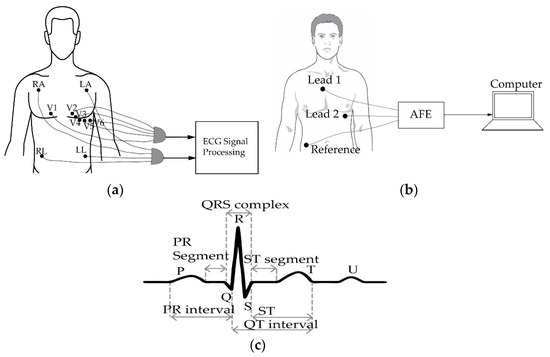
\includegraphics[height=7cm,width=12cm]{Images/chapter1/1-1.jpg}
\caption{(الف) سیستم الکتروکاردیوگرام بالینی؛ (ب) سیستم الکتروکاردیوگرام قابل حمل؛ (ج) نمایش سیگنال \lr{ECG}.\cite{kebe2020human}
}
\end{figure}
\end{center}
\vspace{2cm}



% ====================  اهداف و سوالات پژوهش  ====================

\section{اهداف و سوالات پژوهش}\label{sec1}



هدف اصلی این پژوهش، ارزیابی و تحلیل قابلیت‌های رادارهای \lr{FMCW (Frequency Modulated Continuous Wave)} در اندازه‌گیری ضربان قلب انسان است. این تحقیق به بررسی چگونگی استفاده از این رادارها در شرایط مختلف محیطی و چالش‌های فنی مربوط به کاربرد آنها در اندازه‌گیری ضربان قلب می‌پردازد. به‌طور کلی، اهداف این پژوهش به شرح زیر است:
\begin{enumerate}
    \item \textbf{تحلیل اصول عملکرد رادارهای \lr{FMCW}}: بررسی نحوه عملکرد و ویژگی‌های این نوع رادارها و شبیه‌سازی کاربرد آن‌ها در اندازه‌گیری ضربان قلب.
    \item \textbf{بررسی دقت اندازه‌گیری ضربان قلب با استفاده از رادارهای \lr{FMCW}}: ارزیابی دقت و قابلیت اطمینان اندازه‌گیری ضربان قلب در مقایسه با روش‌های سنتی مانند الکتروکاردیوگرام (\lr{ECG}).
    \item \textbf{بررسی اثرات مختلف محیطی بر عملکرد رادار}: تحلیل تأثیر عواملی مانند حرکت بدن، فاصله، موانع فیزیکی و شرایط محیطی بر دقت اندازه‌گیری ضربان قلب با رادارهای \lr{FMCW}.
    \item \textbf{طراحی سیستم اندازه‌گیری ضربان قلب با رادار \lr{FMCW}}: ارائه یک مدل یا الگوریتم برای بهبود دقت اندازه‌گیری ضربان قلب با استفاده از رادارهای \lr{FMCW} 
    \item \textbf{پیشنهاد کاربردهای پزشکی و بهداشتی رادارهای \lr{FMCW}}: بررسی استفاده از رادارهای \lr{FMCW} برای پایش و نظارت بر سلامت بیماران، به‌ویژه  پزشکی از راه دور.
\end{enumerate}


برای دستیابی به اهداف پژوهش، چندین سوال اصلی مطرح است که پاسخ به آنها می‌تواند به روشن شدن چالش‌ها و فرصت‌های استفاده از رادارهای \lr{FMCW} در اندازه‌گیری ضربان قلب کمک کند:
\begin{enumerate}
    \item چگونه می‌توان از رادارهای \lr{FMCW} برای اندازه‌گیری دقیق ضربان قلب انسان استفاده کرد؟
    \item آیا دقت اندازه‌گیری ضربان قلب با رادار \lr{FMCW} قابل مقایسه با روش‌های سنتی مانند \lr{ECG} است؟
    \item چه عواملی مانند حرکت بدن، فاصله، و موانع فیزیکی می‌توانند بر عملکرد رادار \lr{FMCW} در اندازه‌گیری ضربان قلب تأثیر بگذارند؟
    \item چه چالش‌ها و محدودیت‌هایی در استفاده از رادارهای \lr{FMCW} برای اندازه‌گیری ضربان قلب در شرایط مختلف محیطی وجود دارد؟
    \item چه تکنیک‌هایی می‌توانند دقت اندازه‌گیری ضربان قلب با استفاده از رادارهای \lr{FMCW} را در محیط‌های شلوغ یا پرتحرک بهبود بخشند؟
    \item چه مزایایی در استفاده از رادارهای \lr{FMCW} برای اندازه‌گیری ضربان قلب در مقایسه با روش‌های تهاجمی و تماس فیزیکی وجود دارد؟
    \item چه کاربردهایی برای استفاده از رادارهای \lr{FMCW} در نظارت بر سلامت بیماران و پایش از راه دور در پزشکی وجود دارد؟
\end{enumerate}

% ====================  اهمیت و نوآوری تحقیق ====================
\section{اهمیت و نوآوری تحقیق}\label{sec1}
\subsection{اهمیت تحقیق}\label{sec1}

با پیشرفت‌های روزافزون در تکنولوژی‌های ارتباطی و پردازشی، اندازه‌گیری ضربان قلب به عنوان یک پارامتر حیاتی در تشخیص وضعیت سلامت انسان، همواره در مرکز توجه محققان و پزشکان قرار داشته است. در این راستا، روش‌های سنتی اندازه‌گیری ضربان قلب که معمولاً به تجهیزات خاص یا تماس فیزیکی با بدن مانند الکتروکاردیوگرام (\lr{ECG}) یا پالس اکسیمتر وابسته هستند، می‌توانند برای بیماران دردناک باشند یا حتی در بعضی موارد عملی نباشند. به‌ویژه در محیط‌های بیمارستانی شلوغ یا در هنگام مراقبت‌های از راه دور، این روش‌ها ممکن است کارآیی و دقت کافی نداشته باشند.
با توجه به این محدودیت‌ها، استفاده از تکنولوژی‌های جدید مانند رادارهای \lr{FMCW} به عنوان یک راهکار دقیق برای اندازه‌گیری ضربان قلب، اهمیت ویژه‌ای پیدا کرده است. رادارهای \lr{FMCW} با استفاده از امواج رادیویی قادر به شبیه‌سازی حرکت‌های بسیار کوچک در بدن انسان، مانند تغییرات ناشی از ضربان قلب، هستند. این قابلیت‌ها باعث می‌شود که رادارهای \lr{FMCW} به ابزاری مؤثر در زمینه مراقبت‌های پزشکی از راه دور، پایش سلامت بیماران و حتی در محیط‌های پرتحرک تبدیل شوند.
این تحقیق می‌تواند با بررسی و ارزیابی کاربرد رادارهای \lr{FMCW} در اندازه‌گیری ضربان قلب، کمک شایانی به گسترش کاربرد این تکنولوژی در حوزه‌های پزشکی و بهداشت عمومی کند. با توجه به عدم نیاز به تماس فیزیکی و قابلیت اندازه‌گیری ضربان قلب در شرایط متنوع، این تحقیق می‌تواند زمینه‌ساز تحول در روش‌های نظارت بر سلامت انسان باشد.

\subsection{نوآوری تحقیق}\label{sec2}

نوآوری این تحقیق در استفاده از رادارهای \lr{FMCW}  برای اندازه‌گیری ضربان قلب به‌صورت غیرتماسی و در شرایط مختلف محیطی است. این نوآوری شامل جنبه‌های زیر می‌باشد:
\begin{enumerate}
    \item \textbf{استفاده از رادارهای \lr{FMCW} برای اندازه‌گیری ضربان قلب}: رادارهای \lr{FMCW} تا به امروز بیشتر در زمینه‌های نظامی، فضایی و صنعتی کاربرد داشته‌اند، اما این تحقیق اولین گام در استفاده از این رادارها برای اندازه‌گیری دقیق ضربان قلب انسان است. استفاده از این رادارها به‌عنوان ابزاری دقیق برای پایش سلامت، یک نوآوری در علوم پزشکی به‌شمار می‌رود.
    \item \textbf{اندازه‌گیری ضربان قلب در محیط‌های پرتحرک}: از آنجایی که رادارهای \lr{FMCW} قادر به اندازه‌گیری حرکت‌های بسیار کوچک در بدن هستند، این تحقیق به بررسی توانایی این رادارها در اندازه‌گیری ضربان قلب در شرایطی مانند حرکت بدن، فاصله، یا محیط‌های شلوغ و پرتحرک پرداخته است. این ویژگی می‌تواند تحولی در مراقبت‌های پزشکی از راه دور و نظارت بر وضعیت بیماران در هنگام فعالیت‌های روزمره باشد.
    \item \textbf{کاربرد رادارهای \lr{FMCW} در پایش سلامت از راه دور}: این تحقیق همچنین به بررسی کاربردهای رادارهای \lr{FMCW} در پایش ضربان قلب بیماران از راه دور پرداخته است. در این زمینه، رادارهای \lr{FMCW} می‌توانند به‌عنوان یک ابزار نظارتی بی‌دردسر و دقیق در مراکز درمانی و بیمارستان‌ها، بدون نیاز به تجهیزات اضافی یا تماس فیزیکی، عمل کنند.
    \item \textbf{توسعه الگوریتم‌های پردازش سیگنال برای بهبود دقت اندازه‌گیری}: یکی دیگر از جنبه‌های نوآورانه این تحقیق، طراحی و بهینه‌سازی الگوریتم‌های پردازش سیگنال برای تحلیل داده‌های رادار \lr{FMCW} به منظور افزایش دقت اندازه‌گیری ضربان قلب در شرایط مختلف محیطی است. این الگوریتم‌ها می‌توانند تغییرات کوچک در امواج راداری ناشی از ضربان قلب را از سایر سیگنال‌ها تفکیک کرده و دقت اندازه‌گیری را بهبود بخشند.
\end{enumerate}


% ==================== روش‌شناسی تحقیق   ====================
\section{روش‌شناسی تحقیق} % Corresponds to 1.4
\label{sec:methodology}

\subsection{مقدمه} % Corresponds to 1.4.1
\label{sec:methodology-intro}
روش‌شناسی تحقیق در این مطالعه، شامل طراحی و پیاده‌سازی یک سیستم اندازه‌گیری ضربان قلب مبتنی بر رادار \lr{FMCW} است. این تحقیق به‌منظور ارزیابی دقت، عملکرد و قابلیت‌های رادارهای \lr{FMCW} برای اندازه‌گیری ضربان قلب در شرایط مختلف محیطی و عملیاتی طراحی شده است. در این فصل، به‌تفصیل روش‌ها و مراحل مختلف تحقیق شامل طراحی سیستم، نحوه جمع‌آوری داده‌ها، تحلیل داده‌ها و ارزیابی عملکرد سیستم پرداخته خواهد شد.

\subsection{طراحی سیستم راداری \lr{FMCW}} % Corresponds to 1.4.2
\label{sec:fmcw-system-design}
در ابتدا، یک سیستم راداری \lr{FMCW} برای اندازه‌گیری ضربان قلب طراحی می‌شود. این سیستم شامل اجزای زیر است:
\begin{enumerate}
    \item \textbf{منبع سیگنال راداری}: یک سیگنال مدولاسیون فرکانسی پیوسته تولید می‌شود که فرکانس آن به‌طور پیوسته تغییر می‌کند.
    \item \textbf{آنتن راداری}: برای ارسال و دریافت سیگنال‌های رادیویی به‌کار می‌رود.
    \item \textbf{مدار پردازش سیگنال}: سیگنال‌های دریافتی از آنتن پردازش شده و تغییرات ناشی از ضربان قلب استخراج می‌شود.
    \item \textbf{سیستم تحلیل داده‌ها}: پس از پردازش سیگنال، الگوریتم‌های مختلف برای تحلیل و استخراج ضربان قلب از داده‌های راداری استفاده می‌شود.
\end{enumerate}

\subsection{جمع‌آوری داده‌ها} % Corresponds to 1.4.3
\label{sec:data-collection}
برای جمع‌آوری داده‌ها، آزمایش‌های مختلف با استفاده از رادار \lr{FMCW} در محیط‌های متفاوت طراحی می‌شود. داده‌ها از دو بخش اصلی استخراج می‌شوند:
\begin{itemize}
    \item **داده‌های راداری**: این داده‌ها از سیگنال‌های بازتاب‌شده از بدن انسان که تحت تأثیر ضربان قلب تغییر می‌کنند، به‌دست می‌آید.
    \item **داده‌های مرجع**: برای مقایسه دقت سیستم راداری، از روش‌های سنتی اندازه‌گیری ضربان قلب مانند الکتروکاردیوگرام (\lr{ECG}) یا پالس اکسیمتر به‌عنوان داده‌های مرجع استفاده می‌شود.
\end{itemize}
آزمایش‌ها در شرایط مختلف انجام خواهد شد، از جمله در حالت ایستاده، نشسته و در حال حرکت، تا قابلیت اندازه‌گیری ضربان قلب در شرایط عملیاتی متفاوت ارزیابی گردد.

\subsection{(این بخش را باید بازنویس کنم )تحلیل داده‌ها و پردازش سیگنال} % Corresponds to 1.4.4 - Note: Your numbering was '4.' but should be '1.4.4' as a subsection.
\label{sec:data-analysis-signal-processing}
برای استخراج ضربان قلب از سیگنال‌های راداری، نیاز به استفاده از تکنیک‌های پردازش سیگنال است. این مرحله شامل چندین مرحله مهم است:
\begin{itemize}
    \item **فیلتر کردن سیگنال‌ها**: سیگنال‌های راداری ممکن است حاوی نویزهایی باشند که باید فیلتر شوند. از فیلترهای دیجیتال برای حذف نویزهای اضافی و بهبود دقت اندازه‌گیری استفاده می‌شود.
    \item **تبدیل فوریه**: سیگنال‌های راداری برای استخراج فرکانس تغییرات ضربان قلب به تبدیل فوریه نیاز دارند. این تبدیل به ما کمک می‌کند تا فرکانس ضربان قلب را از سیگنال‌های راداری استخراج کنیم.
    \item **تحلیل زمان-فرکانس**: برای شبیه‌سازی دقیق‌تر رفتار ضربان قلب، از روش‌های زمان-فرکانس مانند تبدیل ویولت برای استخراج ویژگی‌های دقیق‌تر استفاده می‌شود.
\end{itemize}

\subsubsection{ارزیابی دقت و مقایسه با روش‌های سنتی} % This corresponds to 1.4.4.1 (as it's a sub-part of 1.4.4)
\label{sec2}
در این مرحله، دقت سیستم راداری \lr{FMCW} با استفاده از داده‌های مرجع مقایسه می‌شود. برای ارزیابی دقت اندازه‌گیری ضربان قلب، معیارهای زیر در نظر گرفته می‌شوند:
\begin{itemize}
    \item **خطای مطلق اندازه‌گیری (\lr{MAE})**: تفاوت بین ضربان قلب اندازه‌گیری شده توسط رادار \lr{FMCW} و داده‌های مرجع.
    \item **دقت اندازه‌گیری**: درصد انطباق اندازه‌گیری‌ها با داده‌های مرجع.
    \item **پایداری اندازه‌گیری**: ارزیابی اینکه آیا سیستم در شرایط مختلف محیطی، از جمله حرکت بدن یا تغییرات در فاصله، قادر به حفظ دقت خود است یا خیر.
\end{itemize}

\subsection{تحلیل نتایج و بررسی شرایط مختلف} % Corresponds to 1.4.5
\label{sec:results-analysis}
در این بخش، نتایج به‌دست‌آمده از آزمایش‌ها تجزیه و تحلیل می‌شود. نتایج عملکرد رادار \lr{FMCW} در شرایط مختلف مانند ایستاده، نشسته و در حال حرکت، به‌طور جامع بررسی می‌شود. همچنین تأثیر عواملی مانند فاصله، موانع فیزیکی و شرایط محیطی (مانند حضور افراد دیگر یا نویز رادیویی) بر دقت اندازه‌گیری ضربان قلب بررسی خواهد شد.

\subsection{بهینه‌سازی سیستم} % Corresponds to 1.4.6
\label{sec:system-optimization}
در نهایت، بر اساس نتایج به‌دست‌آمده، بهینه‌سازی‌هایی برای سیستم پیشنهاد می‌شود. این بهینه‌سازی‌ها می‌تواند شامل بهبود الگوریتم‌های پردازش سیگنال، بهبود حساسیت راداری، و کاهش اثرات محیطی بر دقت اندازه‌گیری باشد.




% ==================== مروری بر کارهای مرتبط  ====================
\section{مروری بر کارهای مرتبط} % Corresponds to 1.5
\label{sec:related-work}

\subsection{رادارهای پزشکی و کاربردهای آن‌ها} % Corresponds to 1.5.1
\label{sec:medical-radars}

در سال‌های اخیر، فناوری رادار به‌ویژه در کاربردهای پزشکی مورد توجه ویژه‌ای قرار گرفته است.\cite{li2013review} برخلاف کاربردهای سنتی رادار در صنایع نظامی و خودرو، امروزه رادارها در زمینه‌هایی مانند پایش علائم حیاتی (ضربان قلب و نرخ تنفس)، تشخیص سقوط بیماران، شناسایی حرکت‌های غیرارادی بدن، و پایش بیماران در اتاق مراقبت‌های ویژه مورد استفاده قرار می‌گیرند. این سیستم‌ها، برای بیماران با شرایط خاص، نوزادان و سالمندان مزیت چشم‌گیری دارند.
برخی پژوهش‌ها به بررسی عملکرد رادارهای میلی‌متری برای شناسایی علائم حیاتی در اتاق‌های بیمارستانی یا حتی در محیط خانگی پرداخته‌اند. برای مثال، از رادارهای \lr{Doppler} برای اندازه‌گیری نرخ تنفس استفاده شده و مشخص شده که این رادارها قادر به تشخیص تغییرات کوچک در قفسه سینه فرد هستند. همچنین رادارهای \lr{FMCW} و \lr{UWB} در این زمینه در حال رشد چشمگیری‌اند، چرا که قابلیت تفکیک مکانی و حساسیت بالاتری دارند.

\subsection{اندازه‌گیری ضربان قلب با رادار: روش‌های \lr{CW}، \lr{FMCW}، و \lr{UWB}} % Corresponds to 1.5.2
\label{sec:heart-rate-radar-methods}

اندازه‌گیری ضربان قلب با رادار، با استفاده از روش‌های مختلفی امکان‌پذیر است که هرکدام مزایا و محدودیت‌های خاص خود را دارند:
\begin{itemize}
    \item \textbf{رادار موج پیوسته (\lr{CW})}: در این روش، رادار سیگنال سینوسی با فرکانس ثابت ارسال می‌کند و تغییرات فاز سیگنال بازتاب‌شده را برای تشخیص حرکت‌های ظریف بدن (مثل ضربان قلب) تحلیل می‌کند. این روش ساده است، اما توان تفکیک مکانی ندارد و در محیط‌های با چند هدف یا نویز بالا عملکرد خوبی ندارد.
    \item \textbf{رادار \lr{FMCW (Frequency Modulated Continuous Wave)}}: این روش با استفاده از مدولاسیون خطی فرکانس، امکان تخمین فاصله و همچنین استخراج اطلاعات حرکت ظریف را فراهم می‌آورد. رادارهای \lr{FMCW} با دقت بالا می‌توانند ضربان قلب را در فاصله‌های مختلف و بدون تماس ثبت کنند. پژوهش‌هایی مانند \lr{Li et al. (2018)} و \lr{Wang et al. (2020)} به نتایج موفقی در این زمینه دست یافته‌اند و قابلیت استفاده از \lr{FMCW} را در شرایط متحرک یا پرنویز اثبات کرده‌اند.\cite{yue2020non}
    \item \textbf{رادار باند فوق‌گسترده (\lr{UWB})}: این نوع رادار با ارسال پالس‌های کوتاه و پهن‌باند، قادر به اندازه‌گیری دقیق موقعیت و حرکت است. مزیت آن توانایی بالا در تفکیک مکانی و کاهش اثرات تداخل می‌باشد. در عین حال، به دلیل الزامات تنظیمی و پیچیدگی سخت‌افزار، کاربرد آن در عمل ممکن است محدود شود.
\end{itemize}

\subsection{خلأها و چالش‌های موجود} % Corresponds to 1.5.3
\label{sec:gaps-challenges}

با وجود پیشرفت‌های قابل‌توجه در اندازه‌گیری ضربان قلب با استفاده از رادار، همچنان چالش‌ها و خلأهایی در این حوزه باقی مانده است:
\begin{enumerate}
    \item \textbf{نویز و تداخل حرکتی}: یکی از چالش‌های اصلی، تداخل ناشی از حرکت‌های بزرگ بدن یا حضور اشیاء متحرک در محیط است که می‌تواند بر روی سیگنال ضربان قلب اثر بگذارد و دقت اندازه‌گیری را کاهش دهد.
    \item \textbf{تفکیک ضربان قلب از نرخ تنفس}: در بسیاری از موارد، سیگنال‌های ناشی از تنفس قوی‌تر از سیگنال ضربان قلب هستند و استخراج دقیق ضربان قلب نیازمند فیلترینگ دقیق یا استفاده از الگوریتم‌های پردازش سیگنال پیشرفته است.\cite{adib2015smart}
    \item \textbf{نبود مدل استاندارد برای مقایسه عملکرد}: بیشتر تحقیقات از روش‌های خاص خود برای اندازه‌گیری و ارزیابی استفاده کرده‌اند و فقدان یک استاندارد یا دیتاست عمومی باعث دشواری در مقایسه دقیق میان روش‌ها می‌شود.
    \item \textbf{پیاده‌سازی در شرایط واقعی}: بسیاری از مطالعات در محیط‌های کنترل‌شده آزمایشگاهی انجام شده‌اند. پیاده‌سازی موفق در محیط‌های واقعی (مانند اتاق بیمار، خودرو یا منزل) نیازمند بهینه‌سازی طراحی آنتن، مدارات پردازش و حذف نویز محیطی است.
    \item \textbf{نیاز به الگوریتم‌های هوشمند پردازش سیگنال}: برای استخراج دقیق ضربان قلب از داده‌های راداری، به‌ویژه در حضور نویز و حرکات اضافی، نیاز به الگوریتم‌های پیشرفته یادگیری ماشین، پردازش سیگنال تطبیقی و تحلیل چند متغیره احساس می‌شود.
\end{enumerate}



\vspace{2cm}
\begin{center}
\begin{figure}[!h]
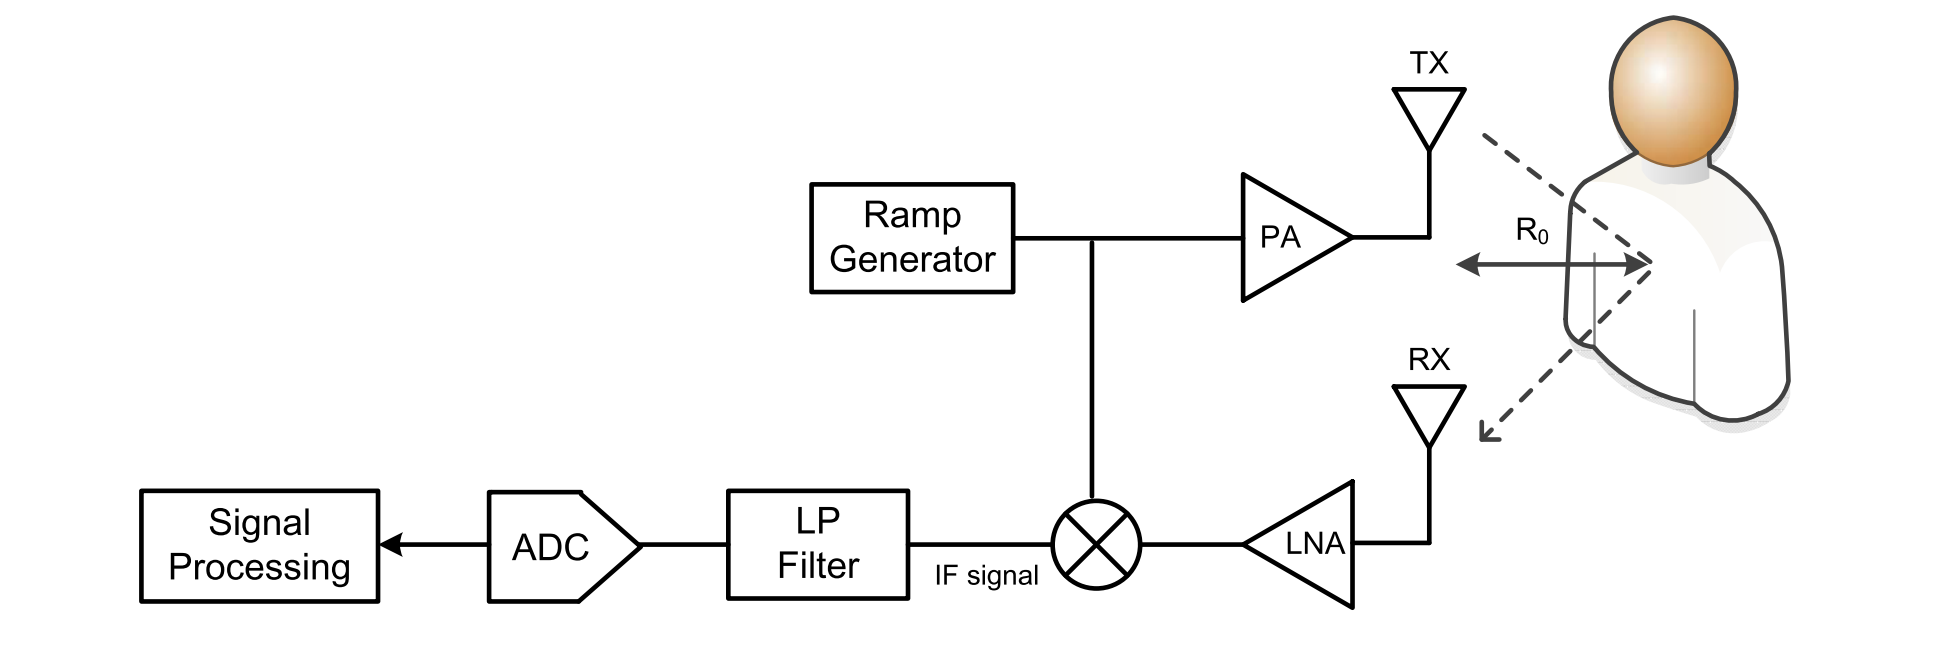
\includegraphics[height=4cm,width=12cm]{Images/chapter1/1-2.png}
\caption{بلاک دیاگرام رادار \lr{fmcw}.\cite{adib2015smart}
}
\end{figure}
\end{center}
\vspace{2cm}



% \chapter{مبانی نظری رادار \lr{FMCW} و فیزیولوژی ضربان قلب}
\label{ch:fmcw-physiology}

% ====================  مقدمه  ====================

\section{مقدمه}
در این فصل به دو محور اصلی پرداخته می‌شود:

بررسی فیزیولوژی ضربان قلب و الگوی حرکتی با تأکید بر ویژگی‌های سیگنال‌های حرکتی (\lr{micro-motions}) قفسه سینه که ناشی از تپش‌های قلب هستند؛

مبانی نظری رادار \lr{FMCW (Frequency-Modulated Continuous-Wave)} و پارامترهای کلیدی طراحی آن تشریح شده و روش‌های پردازش پیشرفته برای جداسازی و اندازه‌گیری دقیق ضربان قلب به‌صورت غیرتماسی ارائه می‌شوند. در بخش اول، با مروری بر مکانیسم انقباض و انبساط میوکارد و انتشار موج پرفیوژن، نشان داده می‌شود که چگونه تغییرات بسیار کوچک موقعیت سطح قفسه سینه (در حد میلی‌متر یا کمتر) حامل اطلاعات حیاتی ضربان و نرخ متغیر قلب است. این تبیین فیزیولوژیک، مبنای انتخاب پارامترهای راداری مناسب را فراهم می‌آورد.

در بخش دوم، اصول کار رادارهای \lr{FMCW} با معرفی سیگنال‌های \lr{Chirp} و رابطه فرکانس \lr{Beat} برای اندازه‌گیری فاصله و سرعت توضیح داده خواهد شد
. سپس پارامترهای پهنای باند (\lr{B})، مدت زمان چرخه (\lr{Tp}) و نسبت سیگنال به نویز (\lr{SNR}) مورد بررسی قرار می‌گیرند که هر یک تأثیر مستقیمی بر دقت فاصله‌سنجی و تشخیص کوچک‌ترین حرکات دارند.

در ادامه، روش‌های متنوع پردازش سیگنال با هدف بهبود جداسازی ضربان قلب از نویز و حرکات مزاحم بدن مرور می‌شوند:
\begin{itemize}
  \item ارتقای تفکیک‌پذیری هم‌زمان فاصله و سرعت در رادارهای قابل پیکربندی
  \item مقایسه کارایی رادارهای داپلر و \lr{FMCW} در پایش علائم حیاتی غیرتماسی
  \item به‌کارگیری نمونه‌برداری انتخابی برای گسترش دامنه سرعت قابل تشخیص
  \item استفاده از رادار میلی‌متری جهت پایش هم‌زمان چند سوژه و کاهش نویز با کمک الگوریتم تجزیه مقادیر منفرد (\lr{SVD})
  \item تحلیل تغییرات درون‌فردی سیگنال‌های سیزموکاردیوگرام
  \item ارائه چارچوب‌های چندهدفه برای استخراج و پایش تغییرات ضربان قلب
\end{itemize}

این ساختار فصل، خواننده را از مبانی فیزیولوژیک تا روش‌های نوین 
پردازش سیگنال راداری هدایت می‌کند و زمینه را برای ارائه روش تحقیق و نتایج تجربی در فصل‌های بعدی فراهم می‌آورد.



% ====================  اصول کار رادار  ====================
\section{اصول کار رادار \lr{FMCW}}\label{sec:fmcw-principles}


\subsection{سیگنال چیپ (\lr{Chirp}) و پهنای باند} % Subsection 2.1.1
\label{sec:chirp-bandwidth}

رادارهای \lr{FMCW (Frequency-Modulated Continuous Wave)} از نوع خاصی از امواج رادیویی استفاده می‌کنند که فرکانس آن‌ها به‌صورت خطی در بازه‌ای از زمان تغییر می‌کند. به این سیگنال‌ها، «چیپ» (\lr{Chirp}) گفته می‌شود. در یک چرخه از عملکرد رادار، سیگنال فرستاده‌شده از نوع خطی صعودی است که در آن فرکانس از یک مقدار آغازین \lr{$f_0$} تا مقدار \lr{$f_0 + B$} در مدت زمان \lr{$T$} افزایش می‌یابد.





\vspace{2cm}
\begin{center}
\begin{figure}[!h]
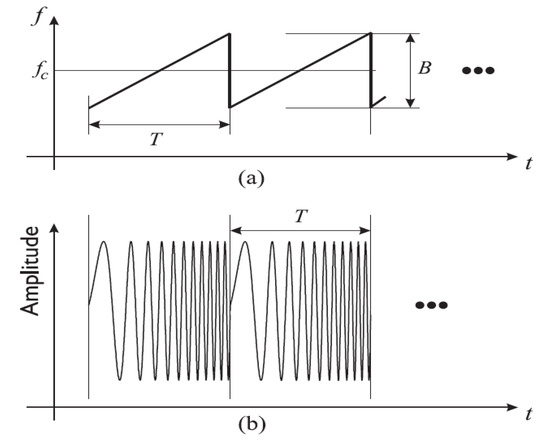
\includegraphics[height=10cm,width=12cm]{Images/chapter2/2-1.jpg}
\caption{(\lr{a}) تغییر فرکانس در طول زمان، (\lr{b}) سیگنال‌های \lr{chirp} لحظه‌ای.
\cite{kebe2020human}
}
\end{figure}
\end{center}
\vspace{2cm}

ویژگی کلیدی این نوع سیگنال در اندازه‌گیری فاصله، قابلیت نمایش موقعیت فاصله‌ای اهداف با استفاده از اختلاف فرکانسی بین سیگنال ارسال‌شده و سیگنال بازتابی است. هنگامی که سیگنال بازتابی از یک هدف با تأخیر زمانی دریافت می‌شود، اختلاف فرکانس بین سیگنال دریافتی و ارسال‌شده (که به آن \lr{beat frequency} گفته می‌شود) مستقیماً با فاصله هدف مرتبط است.


فرکانس \lr{beat} با رابطه زیر تعیین می‌شود:
\begin{equation}
f_b = \frac{2BR}{cT}
\label{eq:beat_frequency}
\end{equation}
\addequation{اختلاف فرکانس بین سیگنال دریافتی و ارسال‌شده}

که در آن:
\begin{itemize}
    \item \lr{$B$}: پهنای باند سیگنال چیپ
    \item \lr{$R$}: فاصله تا هدف
    \item \lr{$c$}: سرعت نور
    \item \lr{$T$}: مدت‌زمان سیگنال
\end{itemize}

 در کاربردهای زیستی مانند پایش ضربان قلب، حرکت‌های بسیار ظریف سطح قفسه سینه (در حد میلی‌متر یا کمتر) باعث ایجاد تغییرات فرکانسی بسیار کوچک در سیگنال برگشتی می‌شود، که با تحلیل دقیق این \lr{beat frequency} می‌توان علائم حیاتی نظیر ضربان قلب را استخراج کرد.
\cite{munoz2018doppler}

در مقاله \cite{neemat2019reconfigurable}، تمرکز بر افزایش قدرت تفکیک (\lr{resolution}) در محور فاصله است. طبق یافته‌های این مقاله، پهنای باند سیگنال چیپ مستقیماً بر توان تفکیک فاصله اثرگذار است.تفکیک فاصله‌ای \lr{$\Delta R$} به‌صورت زیر تعریف می‌شود:
\begin{equation}
\Delta R = \frac{c}{2B}
\label{eq:range_resolution}
\end{equation}
\addequation{رابطه‌ی تفکیک فاصله‌ای در رادار \lr{FMCW}}

بنابراین، افزایش پهنای باند باعث بهبود توانایی سیستم در تمایز اهداف نزدیک به هم می‌شود. در کاربردهای پزشکی مانند اندازه‌گیری ضربان قلب، که در آن سیگنال‌های بسیار ضعیف از حرکت‌های سطحی بدن ثبت می‌شود، این افزایش تفکیک می‌تواند به تفکیک بهتر نویز محیطی از سیگنال واقعی ضربان قلب منجر شود.
همچنین به معرفی پردازش دامنه داپلر قابل پیکربندی (\cite{neemat2019reconfigurable}) پرداخته است که با تغییر معماری فریم‌های چیپ، امکان جداسازی بهتر سیگنال‌های مربوط به تنفس و ضربان قلب فراهم می‌شود. این موضوع در شرایطی که حرکت‌های دیگر بدن وجود دارند (مانند تکان‌های سر یا دست)، اهمیت دوچندان پیدا می‌کند.
در جمع‌بندی این بخش، می‌توان گفت که استفاده از سیگنال‌های چیپ با پهنای باند بالا، نه‌تنها دقت فاصله‌سنجی را در رادارهای \lr{FMCW} افزایش می‌دهد، بلکه با بهره‌گیری از روش‌هایی مانند \lr{Range-Doppler} قابل پیکربندی، تفکیک و تحلیل دقیق‌تری از علائم حیاتی فراهم می‌آورد.

%=================================================================================================


\subsection{آشکارسازی فاصله و سرعت} 
\label{sec:range-velocity-detection}

رادارهای \lr{FMCW (Frequency-Modulated Continuous Wave)} از سیگنال‌های خطی چیپ (\lr{Chirp}) برای اندازه‌گیری فاصله و سرعت استفاده می‌کنند. یکی از ویژگی‌های کلیدی رادارهای \lr{FMCW} توانایی آشکارسازی دقیق فاصله (\lr{Range}) و سرعت (\lr{Doppler Velocity}) اهداف مختلف است. برای دستیابی به این قابلیت، رادار \lr{FMCW} از اصول پیچیده‌ای برای پردازش سیگنال‌ها استفاده می‌کند که در مقایسه با رادارهای \lr{CW (Continuous Wave)} و \lr{Pulse}، مزایای بیشتری را در دقت اندازه‌گیری فراهم می‌آورد.

\subsubsection{آشکارسازی فاصله} % Corresponds to 2.1.2.1
\label{sec:range-detection}

در رادار \lr{FMCW}، فاصله تا هدف از طریق تحلیل فرکانس \lr{beat} که نتیجه اختلاف فرکانس بین سیگنال ارسالی و بازتابی است، محاسبه می‌شود. این اختلاف فرکانسی به‌طور مستقیم با فاصله‌ی هدف مرتبط است و طبق رابطه‌ی زیر تعیین می‌شود:
\begin{equation}
f_b = \frac{2B \cdot R}{cT}
\label{eq:beat_frequency}
\end{equation}
\addequation{رابطه‌ی فرکانس \lr{beat} برحسب فاصله‌ی هدف}

که در آن:
\begin{itemize}
    \item \lr{$f_b$}: فرکانس \lr{beat}،
    \item \lr{$B$}: پهنای باند سیگنال چیپ،
    \item \lr{$R$}: فاصله تا هدف،
    \item \lr{$c$}: سرعت نور،
    \item \lr{$T$}: مدت‌زمان چرخه‌ی سیگنال.
\end{itemize}

\vspace{2cm}
\begin{center}
\begin{figure}[!h]
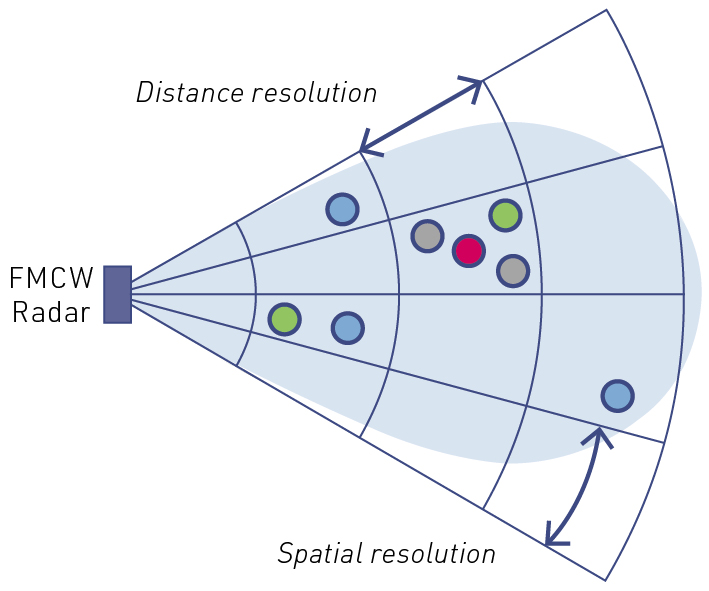
\includegraphics[height=10cm,width=12cm]{Images/chapter2/2-2.jpg}
\caption{تشخیص و تفکیک اهداف مختلف در میدان دید رادار \lr{fmcw}
\cite{rfbeam2024}
}
\end{figure}
\end{center}
\vspace{2cm}

برای دقیق‌تر کردن اندازه‌گیری فاصله در رادارهای \lr{FMCW}، افزایش پهنای باند سیگنال چیپ اهمیت ویژه‌ای دارد. همان‌طور که در مقاله \cite{neemat2019reconfigurable} اشاره شده است، با افزایش پهنای باند \lr{$B$}، دقت تفکیک فاصله بهبود می‌یابد، چرا که تفکیک فاصله \lr{$\Delta R$} به‌طور معکوس با پهنای باند نسبت دارد:
\begin{equation}
\Delta R = \frac{c}{2B}
\label{eq:range_resolution}
\end{equation}
\addequation{رابطه‌ی تفکیک فاصله‌ای برحسب پهنای باند}

این ویژگی، به‌ویژه در کاربردهایی مانند اندازه‌گیری ضربان قلب، که تغییرات فازی کوچکی به‌دلیل حرکت قفسه سینه به وجود می‌آید، بسیار حیاتی است.

\subsubsection{آشکارسازی سرعت} % Corresponds to 2.1.2.2
\label{sec:velocity-detection}

در رادار \lr{FMCW}، سرعت اهداف به کمک اثر داپلر (\lr{Doppler Effect}) و تحلیل فرکانس داپلر استخراج می‌شود.سیگنال‌های بازتابی از اهداف متحرک موجب تغییر در فرکانس آن‌ها می‌شوند که این تغییر به‌عنوان تغییر فرکانس داپلر در سیگنال دریافت‌شده ظاهر می‌شود. فرکانس داپلر با سرعت هدف مرتبط است \cite{kwak2024adjusting} و به‌صورت زیر محاسبه می‌شود:
\begin{equation}
f_d = \frac{2v}{\lambda}
\label{eq:doppler_frequency}
\end{equation}
\addequation{رابطه‌ی فرکانس داپلر برحسب سرعت هدف و طول‌موج}

که در آن:
\begin{itemize}
    \item \lr{$f_d$}: فرکانس داپلر،
    \item \lr{$v$}: سرعت نسبی هدف نسبت به رادار،
    \item \lr{$\lambda$}: طول‌موج سیگنال رادار.
\end{itemize}

یکی از چالش‌ها در سیستم‌های رادار \lr{FMCW}، محدودیت دامنه سرعت قابل تشخیص است. سرعت‌های بسیار پایین یا سرعت‌های بالا ممکن است باعث شود که سیگنال داپلر تغییرات نامشخص یا حتی معکوس داشته باشد، که در نتیجه منجر به از دست رفتن سیگنال یا کاهش دقت در تشخیص سرعت می‌شود.
برای حل این مشکل، مقاله \cite{kwak2024adjusting} به تکنیک‌هایی برای نمونه‌برداری انتخابی (\lr{Selective Sampling}) اشاره کرده است که با تنظیم فواصل نمونه‌برداری، می‌توان دامنه سرعت قابل تشخیص را افزایش داد. به این معنا که می‌توان سیستم رادار را طوری تنظیم کرد که دامنه‌ای گسترده‌تر از سرعت‌ها را با دقت بیشتری اندازه‌گیری کند، بدون اینکه از کیفیت اندازه‌گیری فاصله کاسته شود.


\subsubsection{پیشرفت‌ها در پردازش دامنه داپلر و فاصله} % Corresponds to 2.1.2.3
\label{sec:advanced-range-doppler-processing}

یکی دیگر از چالش‌ها در سیستم‌های رادار \lr{FMCW}، نیاز به پردازش دقیق و بهینه داده‌ها در دامنه داپلر و فاصله است. مقاله \cite{neemat2019reconfigurable}  توضیح می‌دهد که استفاده از پردازش دامنه داپلر قابل پیکربندی می‌تواند به بهبود تفکیک سرعت و فاصله در سیستم‌های راداری \lr{FMCW} کمک کند. این روش با تنظیم پارامترهای سیستم در هر فریم، به رادار اجازه می‌دهد که دامنه‌های وسیع‌تری از سرعت و فاصله را پردازش کند و در عین حال از تداخل‌های نامطلوب جلوگیری کند.
پردازش دامنه داپلر به سیستم‌های راداری اجازه می‌دهد تا علاوه بر اندازه‌گیری فاصله، سرعت حرکت اهداف مانند حرکت قفسه سینه در هنگام ضربان قلب را به‌طور دقیق شبیه‌سازی و اندازه‌گیری کنند. این قابلیت برای کاربردهای پزشکی مانند پایش ضربان قلب در شرایط مختلف حرکت یا تغییر موقعیت بدن، به‌ویژه در مواقعی که حرکت‌های بدن موجب اختلال در سیگنال می‌شود، بسیار مفید است.


%=================================================================================================




% ====================  پارامترهای کلیدی در طراحی  ====================
\section{پارامترهای کلیدی در طراحی \lr{FMCW} (\lr{B}, \lr{$T_p$}, \lr{SNR} و ...)}\label{sec:fmcw-key-parameters} % Corresponds to 2.2


در سیستم‌های رادار \lr{FMCW}، طراحی بهینه و انتخاب مناسب پارامترهای مختلف تأثیر بسزایی در دقت اندازه‌گیری، عملکرد، و قابلیت تشخیص اهداف دارد. در این بخش، به بررسی پارامترهای کلیدی در طراحی سیستم‌های \lr{FMCW} پرداخته خواهد شد که به‌ویژه در کاربردهای پزشکی مانند اندازه‌گیری ضربان قلب اهمیت زیادی دارند. این پارامترها شامل پهنای باند (\lr{B})، مدت زمان چرخه (\lr{$T_p$})، نسبت سیگنال به نویز (\lr{SNR}) و برخی دیگر از فاکتورهای مهم در طراحی سیستم راداری هستند.

\subsection{پهنای باند (\lr{B})} % Corresponds to 2.2.1
\label{sec:bandwidth}

پهنای باند \lr{$B$} یکی از مهم‌ترین پارامترها در طراحی سیستم‌های راداری \lr{FMCW} است. افزایش پهنای باند منجر به دقت بالاتر در اندازه‌گیری فاصله و تفکیک بهتر اهداف می‌شود. طبق مقاله \cite{islam2020non}، با افزایش پهنای باند، سیستم قادر به تمایز بهتر میان اهداف نزدیک به هم خواهد بود که این ویژگی در اندازه‌گیری‌های پزشکی بسیار حائز اهمیت است، به‌ویژه برای تمایز ضربان قلب از دیگر سیگنال‌های جسمی.
رابطه‌ی پهنای باند با تفکیک فاصله به‌صورت زیر بیان می‌شود:
\begin{equation}
\Delta R = \frac{c}{2B}
\label{eq:range_resolution_bandwidth}
\end{equation}
\addequation{رابطه‌ی میان پهنای باند و تفکیک فاصله‌ای}

که در آن \lr{$\Delta R$} تفکیک فاصله و \lr{$c$} سرعت نور است. این رابطه نشان می‌دهد که با افزایش \lr{$B$}، تفکیک فاصله بهبود می‌یابد و دقت اندازه‌گیری افزایش می‌یابد. در اندازه‌گیری ضربان قلب، این ویژگی باعث می‌شود که سیستم بتواند تغییرات جزئی در حرکت بدن که ناشی از ضربان قلب است، با دقت بیشتری شبیه‌سازی کند.

\subsection{مدت زمان چرخه (\lr{$T_p$})} % Corresponds to 2.2.2
\label{sec:chirp-duration}

مدت زمان چرخه \lr{$T_p$} که به آن مدت زمان مدولاسیون نیز گفته می‌شود، تأثیر زیادی بر عملکرد رادارهای \lr{FMCW} دارد. مدت زمان مدولاسیون، مدت زمانی است که سیگنال فرکانس خطی تغییر می‌کند. طبق مقاله \cite{lv2024millimeter}، افزایش مدت زمان \lr{$T_p$} موجب افزایش دقت در شبیه‌سازی تغییرات ضربان قلب می‌شود، زیرا طولانی‌تر شدن چرخه سیگنال امکان تحلیل دقیق‌تر تغییرات سیگنال‌های برگشتی را فراهم می‌آورد.
با توجه به این مقاله، افزایش مدت زمان چرخه می‌تواند باعث بهبود توانایی سیستم در تمایز نویز از سیگنال اصلی ضربان قلب شود. همچنین، انتخاب مدت زمان مناسب برای مدولاسیون سیگنال، ارتباط مستقیمی با دقت اندازه‌گیری سرعت و تفکیک داپلر دارد.

\subsection{نسبت سیگنال به نویز (\lr{SNR})} % Corresponds to 2.2.3
\label{sec:snr}

یکی از چالش‌های اصلی در سیستم‌های راداری \lr{FMCW}، حفظ نسبت سیگنال به نویز (\lr{SNR}) مناسب است. \lr{SNR} یکی از عوامل مهمی است که کیفیت داده‌های دریافتی و دقت اندازه‌گیری را تحت تأثیر قرار می‌دهد. سیستم‌های راداری با \lr{SNR} پایین قادر به تشخیص دقیق تغییرات کوچک در سیگنال‌های برگشتی نخواهند بود، که این مشکل در اندازه‌گیری ضربان قلب در شرایط مختلف محیطی، به‌ویژه در محیط‌های پر نویز مانند بیمارستان‌ها یا محیط‌های شلوغ، به‌وضوح مشاهده می‌شود.
مقاله \cite{islam2020non} به این موضوع پرداخته و اشاره می‌کند که برای پایش علائم حیاتی به‌ویژه ضربان قلب، لازم است که \lr{SNR} به‌گونه‌ای تنظیم شود که سیگنال‌های مرتبط با ضربان قلب به وضوح از نویزهای دیگر تمایز یابند. یکی از روش‌های پیشنهادی برای بهبود \lr{SNR}، استفاده از تکنیک‌های پردازش سیگنال پیشرفته و فیلترینگ هوشمند است.
بهبود \lr{SNR} معمولاً با استفاده از افزایش پهنای باند (\lr{B})، بهبود الگوریتم‌های پردازش سیگنال و افزایش قدرت سیگنال‌های ارسالی امکان‌پذیر است. این کار می‌تواند باعث کاهش اثرات نویز محیطی بر روی داده‌های دریافتی شود.

\subsection{سایر پارامترهای طراحی} % Corresponds to 2.2.4
\label{sec:other-design-parameters}

علاوه بر پارامترهای فوق، در طراحی سیستم‌های \lr{FMCW} برای اندازه‌گیری ضربان قلب، دیگر پارامترها نیز باید در نظر گرفته شوند. برای مثال:
\begin{itemize}
    \item \textbf{آنتن راداری}: طراحی آنتن با قابلیت پوشش‌دهی مناسب برای اندازه‌گیری دقیق اهداف با فاصله‌های مختلف، یکی از ارکان کلیدی طراحی سیستم رادار \lr{FMCW} است.
    \item \textbf{توان سیگنال ارسالی}: میزان توان سیگنال ارسال‌شده می‌تواند بر کیفیت داده‌های دریافتی و حساسیت سیستم تأثیرگذار باشد.
    \item \textbf{پردازش سیگنال تطبیقی}: استفاده از الگوریتم‌های تطبیقی برای فیلتر کردن نویز و شبیه‌سازی دقیق‌تر ضربان قلب می‌تواند به افزایش دقت سیستم کمک کند.
\end{itemize}




% ====================  نتیجه‌گیری  ====================
\section{نتیجه‌گیری}
در پایان این فصل روشن شد که رادارهای \lr{FMCW} با بهره‌گیری از سیگنال‌های \lr{Chirp} و تحلیل \lr{Range–Doppler} می‌توانند حرکات بسیار کوچک ناشی از ضربان قلب را با دقت میلی‌متری تشخیص دهند. افزایش پهنای باند و طول چرخه مدولاسیون (\lr{Tp}) به‌طور مستقیم دقت فاصله‌سنجی را بهبود می‌بخشد، در حالی که حفظ نسبت سیگنال به نویز (\lr{SNR}) بالا برای جداسازی ضربان از نویز محیطی و حرکات تصادفی بدن حیاتی است.

پیشرفت‌های اخیر در پردازش دوبعدی \lr{Range–Doppler} \cite{neemat2019reconfigurable} و نمونه‌برداری انتخابی \cite{kwak2024adjusting} دامنه سرعت قابل اندازه‌گیری را گسترش داده و امکان پایش ضربان قلب در شرایط محیطی و سوژه‌های متحرک بیشتر را فراهم کرده‌اند. روش‌های کاهش نویز مبتنی بر تجزیه مقادیر منفرد (\lr{SVD}) \cite{lv2024millimeter} و بررسی اثرات تغییرات درون‌فردی سیگنال‌های \lr{seismocardiogram} \cite{demirsoy2024investigating} نیز دقت تخمین نرخ ضربان و \lr{HRV} را ارتقاء داده‌اند.

علاوه بر این، کاربرد رادار میلی‌متری در پایش چندسوژه‌ای \cite{islam2020non} و تشخیص چندهدفه \lr{HRV} \cite{xu2024health} نشان داده که با طراحی مناسب آنتن و الگوریتم‌های هوشمند، می‌توان به راه‌حل‌های غیرتماسی دقیق و کارآمد برای کاربردهای پزشکی دست یافت. با این وجود، چالش‌هایی نظیر تداخل متقابل میان سوژه‌ها، کاهش \lr{SNR} در محیط‌های شلوغ و پیچیدگی محاسباتی پردازش \lr{Range–Doppler} همچنان باقی است.

\begin{figure}[ht]
    \centering
    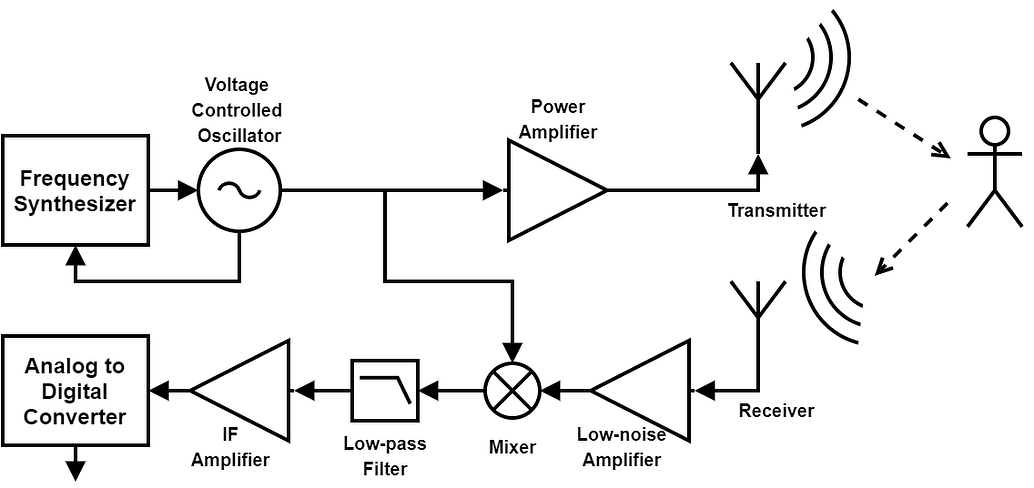
\includegraphics[width=0.7\linewidth]{Images/chapter2/2-3.png}
    \caption{اندازه‌گیری علائم حیاتی با استفاده از رادار \lr{mmWave FMCW} \cite{digikey_fmcw}.}
    \label{fig:fmcw_vitals}
\end{figure}

\vspace{5cm}

فصل بعدی با تکیه بر این مبانی، روش پیشنهادی پژوهش را تشریح خواهد کرد، که در آن با طراحی آزمایش و انتخاب پارامترهای بهینه رادار، تلاش می‌شود محدودیت‌های مطرح‌شده برطرف گردد و کارایی سیستم در پایش ضربان قلب واقعی ارزیابی شود.




% 
\chapter{طراحی سیستم و پیاده‌سازی}

% ====================  مقدمه  ====================
\section{مقدمه}\label{sec:intro-cap3}

% در سال‌های اخیر، نظارت مداوم بر علائم حیاتی انسان (ضربان قلب و نرخ تنفس) به‌عنوان ابزاری کلیدی در تشخیص به‌موقع حوادث حاد و پیش‌بینی زودهنگام وخامت شرایط بالینی مطرح شده است. روش‌های مرسوم مبتنی بر تماس، نظیر \lr{ECG} و \lr{PPG}، اگرچه دقت بالایی ارائه می‌دهند، اما به دلیل نیاز به تماس مستقیم با پوست، در شرایطی نظیر سوختگی، زخم‌های پوستی یا پاندمی‌ها می‌توانند کارآمدی و ایمنی کافی را نداشته باشند.

% در این راستا، رادارهای غیرتماسی مبتنی بر امواج \lr{میلی‌متری‌موج (mmWave)} به دلیل نفوذپذیری مطلوب در بافت‌های سطحی و مقاومت بالا در برابر تغییرات نوری و دمای محیط، به‌عنوان جایگزینی مناسب شناخته شده‌اند. میان انواع مختلف معماری‌های راداری، \lr{FMCW} به‌واسطه مدولاسیون فرکانس خطی، قابلیت تفکیک اهداف چندگانه و همزمان سنجش فاصله و حرکت را فراهم می‌آورد، که در پیاده‌سازی‌های غیرتماسی علائم حیاتی مزایای چشمگیری دارد.

% متون مروری اخیر نشان می‌دهند که تحقیقات متعددی به مقایسه و تحلیل معماری‌های \lr{CW}، \lr{FMCW} و \lr{UWB} پرداخته‌اند. برای نمونه، \lr{Liebetruth} و همکاران (2024) مروری سیستماتیک بر اندازه‌گیری ضربان قلب و تنفس با رادار ارائه داده‌اند و بر نقش متمایز مدولاسیون فرکانس در حذف اختلال‌های محیطی تأکید کرده‌اند. همچنین، \lr{Bin Obadi} و همکاران (2021) در یک مرور جدید، علاوه بر بررسی معماری‌های مختلف، به پیاده‌سازی نرم‌افزاری روی \lr{FPGA} و چالش‌های آن پرداخته‌اند.

% با این حال، اگرچه مطالعات بسیاری بر روی تخمین ضربان قلب و نرخ تنفس متمرکز شده‌اند، تحلیل جامعی از تأثیر پارامترهای فرکانس حامل و پهنای باند بر دقت اندازه‌گیری علائم حیاتی و نیز بررسی کامل جنبه‌های ایمنی و انطباق با استانداردهای پزشکی تا پیش از این کم‌تر انجام شده است. این شکاف پژوهشی انگیزه‌ای قوی برای ارائه یک بررسی متمرکز بر کاربرد رادارهای \lr{FMCW} در پزشکی ایجاد می‌کند.

% در ادامه، ابتدا مبانی فیزیکی و اصول کار رادارهای \lr{FMCW} همراه با بررسی تاریخچه کاربرد آن‌ها در پایش حیاتی بدن مرور خواهد شد. سپس تحولات کلیدی در الگوریتم‌های پردازش سیگنال و پروژه‌های عملی پیاده‌سازی سخت‌افزاری مورد بحث قرار می‌گیرند، تا زمینه‌ای روشن برای طراحی سیستم پیشنهادی این پایان‌نامه فراهم آید.


پایش مداوم علائم حیاتی به‌صورت غیرتماسی، چه در بخش‌های مراقبت ویژه و چه در پایش خانگی بیماران مزمن، نیازمند فناوری‌ای است که هم دقت بالای الکترودهای تماسی را داشته باشد و هم زحمت کمتری برای بیمار ایجاد کند. در میان سه معماری متداول راداری—\lr{CW}، \lr{UWB} و \lr{FMCW}—معماری \lr{FMCW} با ترکیب مدولاسیون خطی فرکانس و پردازش \lr{Beat Signal}، امکان اندازه‌گیری همزمان فاصله و ریزحرکت سطح قفسهٔ سینه را با پیچیدگی سخت‌افزاری قابل قبولی فراهم می‌کند؛ در نتیجه، خطاهای نقطهٔ کور \lr{CW} و محدودیت برد \lr{UWB} تا حد زیادی برطرف می‌شوند.

این فصل ابتدا نشان می‌دهد که چگونه پهنای باند مدولاسیون بر تفکیک‌پذیری فاصله اثر می‌گذارد:

\begin{equation}
\Delta R \approx \frac{c}{2B}
\label{eq:range_resolution}
\end{equation}
\addequation{اثر پهنای باند مدولاسیون بر تفکیک‌پذیری فاصله در سامانه‌های راداری}

و چرا بازه‌ی \lr{1–4 GHz} برای فواصل پزشکی \lr{0.5} تا \lr{3} متر کافی است. سپس به این نکته پرداخته می‌شود که افزایش فرکانس حامل در طیف میلی‌متری، طول موج را کوتاه و حساسیت فاز را افزایش می‌دهد؛ نتایج آزمایش روی رادارهای \lr{60 GHz} و \lr{120 GHz} نشان داده است که دقت اندازه‌گیری ضربان قلب در حدود $\pm 3.1$ \lr{bpm} و خطای تنفس کمتر از \lr{2 brpm} باقی می‌ماند، در حالی که سیستم \lr{24 GHz} به‌دلیل پروفایل نویز بالا کارایی ضعیف‌تری از خود نشان می‌دهد.

بر این مبنا، سخت‌افزار ارائه‌شده در این فصل بر پایه‌ی چیپ \lr{TI IWR1642} با آرایه‌ی مجتمع \lr{MIMO}، توان مصرفی کمتر از \lr{30 mW} و ساختار برد ارزیابی مدولار طراحی شده است؛ انتخابی که امکان جداسازی چند بیمار، اندازه‌ی کوچک، و سازگاری با باتری‌های پوشیدنی را فراهم می‌کند.

در ادامه، زنجیره‌ی پردازش شامل استخراج \lr{Beat Signal}، کالیبراسیون \lr{DC}، بازکردن فاز، فیلتر باندگذر تنفس و ضربان، سرکوب حرکات، و استفاده از الگوریتم \lr{Health-VMD} برای تخمین \lr{HRV} شرح داده می‌شود.

در نهایت، ملاحظات ایمنی، محدودیت توان تابشی، و مسیر اخذ مجوزهای بالینی تکمیل‌کننده‌ی چرخه‌ی طراحی سیستم به‌شمار می‌آیند.


% ====================  مقایسه رادارها  ====================
\section{مقایسه معماری‌های راداری (\lr{FMCW، CW، UWB})}
\label{sec:radar-architecture-comparison}

در این بخش سه معماری اصلی راداری که در سامانه‌های غیرتماسی پایش علائم حیاتی کاربرد دارند \lr{CW (Continuous Wave)}، \lr{FMCW (Frequency-Modulated Continuous Wave)} و \lr{UWB (Ultra-Wideband)}از نظر اصول کاری، پیچیدگی پیاده‌سازی و عملکرد مقایسه می‌شوند.

\subsection{اصول کار معماری‌ها}
\label{sec:principles}

در رادارهای \lr{CW}، سیگنال با فرکانس ثابت و تابش مداوم فرستاده می‌شود و تغییر فاز سیگنال بازتابی به‌عنوان نشانگر حرکت سطح قفسه سینه تحلیل می‌گردد. این سادگی سخت‌افزاری، هزینه و توان مصرفی پایین را فراهم می‌کند؛ اما نقاط کور عمده آن عدم توان تعیین فاصله دقیق و حساسیت بالا به نویزهای چندمسیره است.
\cite{frazao2024radar}

در معماری \lr{FMCW}، فرکانس حامل به‌صورت خطی روی زمان مدوله می‌شود و با تطبیق سیگنال ارسالی و دریافتی (\lr{Beat Signal}) می‌توان هم فاصله و هم سرعت حرکت را استخراج کرد. پهنای باند مدولاسیون رابطه ­مستقیمی با رزولوشن فاصله‌ای دارد:

\begin{equation}
\Delta R = \frac{c}{2B}
\label{eq:range_resolution_bandwidth}
\end{equation}
\addequation{رابطه‌ی میان پهنای باند و تفکیک فاصله‌ای}

و به‌دلیل مدولاسیون فرکانس، این معماری در برابر نویز های محیطی مقاوم‌تر است.
\cite{frazao2024radar}

معماری \lr{UWB} با ارسال پالس‌های کوتاه و گسترده‌پهنای‌باند، تأخیر انتشار موج را برای تخمین فاصله می‌سنجد. گرچه دقت فاصله‌یابی آن بالاست، سخت‌افزار پیچیده و نیاز به پردازش‌های سنگین سیگنال از موانع عمده کاربردهای بالینی آن است.
\cite{paterniani2023radar}

\subsection{مزایا و محدودیت‌ها}
\label{sec:advantages-limitations}

\begin{itemize}
    \item \textbf{\lr{CW}}: کم‌هزینه و ساده؛ مناسب کاربردهای اولیه اما فاقد جداسازی اهداف و مقاومتی اندک در برابر \lr{Multipath Clutter}.
    \item \textbf{\lr{FMCW}}: توازن مطلوب بین سخت‌افزار و قابلیت‌های فاصله‌یابی و تفکیک چندهدفه. پهنای باند بزرگ‌تر، رزولوشن بالاتر و حذف اغتشاشات ناشی از بازتاب‌های ناخواسته را فراهم می‌کند.
    \item \textbf{\lr{UWB}}: دقت بسیار بالا در اندازه‌گیری تأخیر انتشار و امکان نفوذ از موانع جدار نازک؛ اما طراحی آنتن و پردازش دیجیتال پیچیده، هزینه و مصرف انرژی را افزایش می‌دهد.
\end{itemize}


\begin{figure}[ht]
    \centering
    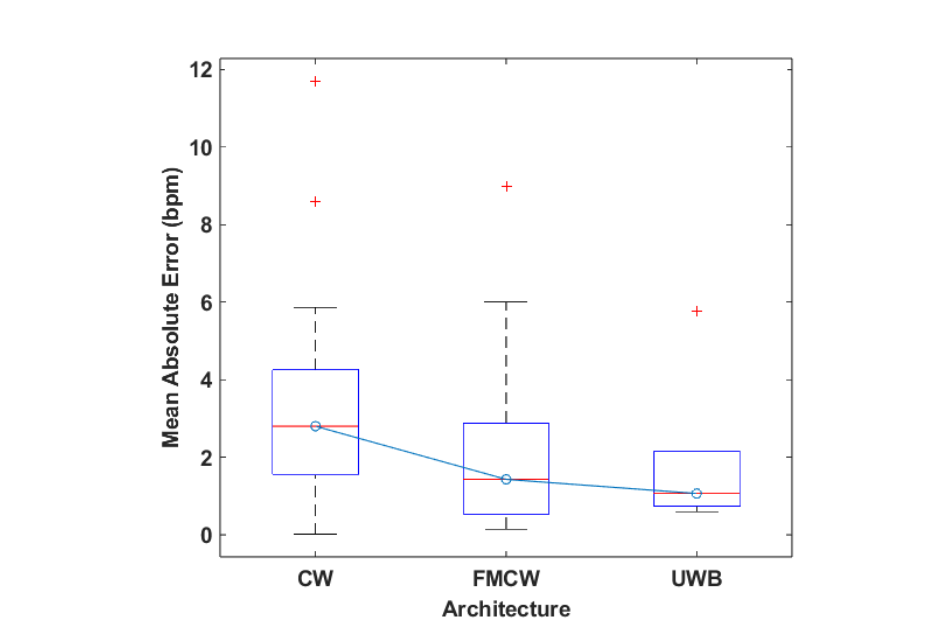
\includegraphics[width=0.7\linewidth]{Images/chapter3/3-2.png}
    \caption{ نمودار جعبه‌ای مقادیر \lr{MAE} برای هر معماری.\cite{frazao2024radar}.}
    \label{fig:fmcw_vitals}
\end{figure}

\subsection{عملکرد آزمایشگاهی و خطاهای اندازه‌گیری}
\label{sec:experimental-performance}

بررسی داده‌های منتشرشده در ۵۶ مطالعه‌ی اندازه‌گیری ضربان قلب نشان می‌دهد که معماری \lr{FMCW} کمترین میانه‌ی خطای مطلق (\lr{MAE}) را دارد، در حالی که \lr{CW} بیشترین میانه‌ی خطا را به خود اختصاص داده است. اگرچه \lr{UWB} در مقایسه‌ی تعداد مطالعات کمتر است، دامنه خطای این معماری کوچک‌تر بوده اما برای تأیید برتری آن نیاز به مطالعات بیشتر است.

به‌طور خاص، در شکل جعبه‌ای (\lr{Boxplot}) مقایسه خطاها، معماری \lr{CW} دارای بالاترین میانه و دامنه‌ی گسترده‌تری از خطا است، در حالی که \lr{FMCW} توزیع خطا فشرده‌تر و \lr{UWB} پایین‌ترین مقادیر حداکثر خطا را نشان می‌دهد. این نتایج گویای برتری معماری \lr{FMCW} در سنجش غیرتماسی ضربان قلب به‌واسطه‌ی مقاومت آن در برابر نویز و تداخل محیطی است.

% \subsection{نتیجه‌گیری موقت}
% \label{sec:interim-conclusion}

% با توجه به مقایسه‌ی مزایا، معایب و داده‌های تجربی، معماری \lr{FMCW} گزینه‌ی اول برای سامانه‌های پزشکی غیرتماسی محسوب می‌شود. \lr{CW} علیرغم سادگی، به‌دلیل عدم امکان تفکیک فاصله و حساسیت بالا به نویز به‌عنوان جایگزین دوم مطرح است و \lr{UWB}، هرچند پتانسیل دقت بالایی دارد، به‌علت پیچیدگی سخت‌افزاری و کمبود مطالعات بالینی گسترده، هنوز در مرحله آزمایشگاهی قرار دارد. در فصل‌های بعدی، بسته به نیازمندی‌های بالینی و محدودیت‌های سخت‌افزاری، انتخاب معماری مناسب برای طراحی سامانه‌ی پایان‌نامه تشریح خواهد شد.


% ====================  انتخاب فرکانس و پهنای باند مناسب  ====================
\section{انتخاب فرکانس و پهنای باند مناسب}
\label{sec:frequency-band-selection}

\subsection{نقش پهنای باند در رزولوشن فاصله‌ای و برد آشکار}
پهناي باند مدولاسیون (\lr{B}) در رادارهای \lr{FMCW} تعیین‌کننده‌ی رزولوشن فاصله‌ای است. به‌طور دقیق، رزولوشن فاصله‌ای با رابطه
\begin{equation}
\Delta R \approx \frac{c}{2B}
\end{equation}
محاسبه می‌شود؛ به‌عبارت دیگر، افزایش \lr{B} موجب کوچک‌تر شدن $\Delta R$ و توانایی تفکیک اهداف نزدیک‌تر می‌شود. از سوی دیگر، بزرگ‌تر شدن پهنای باند می‌تواند برد آشکار ($R_\text{\lr{max}}$) را کاهش دهد، مگر آنکه تعداد نمونه‌ها در هر چیپ (\lr{N}) یا نرخ نمونه‌برداری افزایش یابد، چرا که
\begin{equation}
R_\text{\lr{max}} = \frac{c\,N}{4B}\,.
\end{equation}

در کاربردهای پزشکی غیرتماسی که فاصله‌ی بیمار تا رادار معمولاً در محدوده‌ی \lr{0.5–3 } متر قرار دارد، پهنای باند \lr{1–4 GHz} معمولاً کفاف رزولوشن  و برد آشکار کافی را می‌دهد.

\subsection{تأثیر فرکانس حامل بر حساسیت فاز و عمق نفوذ}
انتخاب فرکانس حامل ($f_c$) در طیف \lr{mmWave} (\lr{30–300 GHz}) به دلیل تأثیر مستقیم بر حساسیت فاز به تغییرات  کوچک‌تر از میلی‌متر و عمق نفوذ الکترومغناطیسی دارای اهمیت است. با افزایش $f_c$ و کاهش طول موج ($\lambda = c/f_c$)، تغییرات کوچک دیواره قفسه‌ی سینه به تغییر فاز بزرگ‌تر تبدیل می‌شوند که استخراج ضربان قلب را دقیق‌تر می‌کند. از سویی دیگر، نفوذپذیری پوست با افزایش فرکانس کاهش می‌یابد (برای مثال عمق نفوذ از \lr{2.7 mm} در \lr{10 GHz} به \lr{0.5 mm} در \lr{60 GHz} می‌رسد)، اما بازتاب از سطح پوست قوی‌تر شده و تأثیر پوشش‌های پارچه‌ای ناچیز می‌گردد.

در مطالعه‌ی مقایسه‌ای بر روی سه رادار کم‌مصرف \lr{FMCW} با فرکانس‌های \lr{24}، \lr{60} و \lr{120 GHz}، نتایج زیر گزارش شده است:
\begin{itemize}
  \item نرخ تنفس (\lr{RR}) با خطای مطلق میانگین (\lr{MAE}) کمتر از \lr{2 brpm} برای هر سه سیستم؛
  \item ضربان قلب (\lr{HR}) با \lr{MAE} برابر $1.8 \pm 3.1$ \lr{bpm} برای سیستم \lr{60 GHz} و $3.2 \pm 5.3$ \lr{bpm} برای سیستم \lr{120 GHz}؛
  \item اما سیستم \lr{24 GHz} به‌دلیل پروفایل نویز بالا، \lr{MAE} حدود \lr{9.0 bpm} داشت.
\end{itemize}

این داده‌ها نشان می‌دهد که انتخاب فرکانس حامل در بازه‌ی \lr{60–120 GHz} می‌تواند به‌طور قابل‌توجهی دقت استخراج علائم حیاتی را افزایش دهد، به‌ویژه زمانی که محدودیت‌های سخت‌افزاری و مصرف توان نیز باید در نظر گرفته شوند.

\subsection{موازن‌سازی در کاربردهای عملی}
اگرچه فرکانس‌های بالاتر (بیش از \lr{60 GHz}) دقت بالاتری ارائه می‌دهند، پیاده‌سازی آنتن و مصرف توان آن‌ها چالش‌برانگیز است. رادارهای کم‌مصرف با توان ده‌ها میلی‌وات و پهنای باند چندگیگاهرتز، نقطه‌ی توازنی میان دقت بالا و قابلیت پیاده‌سازی پوشیدنی فراهم می‌کنند. برای بسیاری از کاربردهای بالینی نظیر نظارت بر بیماران در تخت با پوشش لباس یا ملحفه استفاده از فرکانس‌های میانی (\lr{60–80 GHz}) توصیه می‌شود، چرا که علاوه بر حساسیت فاز مناسب، عمق نفوذ کافی و هزینه‌ی معقول سخت‌افزاری را نیز تأمین می‌کنند.


% ====================  معماری سخت‌افزاری  ====================
\section{طراحی سخت‌افزار و معماری سیستم}

در این فصل، جزئیات پیاده‌سازی سخت‌افزار سامانه مبتنی بر رادار \lr{FMCW} جهت اندازه‌گیری غیرتماسی علائم حیاتی تشریح می‌شود. ابتدا انتخاب چیپ‌ست راداری و پیکربندی آن بررسی می‌شود، سپس چگونگی ساختاربندی ماژول‌ها و ادغام آن‌ها در یک برد ارزیابی به همراه مشخصات آنتن و مصرف توان بیان می‌گردد. در نهایت، معماری \lr{MIMO} و مزایای آن در جداسازی چندشخص مورد بحث قرار می‌گیرد.

\subsection{انتخاب چیپ‌ست رادار و پیکربندی اولیه}

برای پیاده‌سازی رادار \lr{FMCW}، دو رویکرد اصلی مشاهده شده است:

\begin{itemize}
  \item چیپ‌های کم‌مصرف \lr{BGT} از شرکت \lr{Infineon} در فرکانس‌های ۲۴، ۶۰ و ۱۲۰ گیگاهرتز؛
  \item چیپ \lr{IWR1642} از شرکت \lr{Texas Instruments} در باند ۷۷–۸۱ گیگاهرتز.
\end{itemize}
در مجموعه آزمایشات اولیه، سه رادار \lr{BGT24}، \lr{BGT60} و \lr{BGT120} با بهره‌گیری از بردهای ارزیابی ماژولار استفاده شدند. هر کدام از این سیستم‌ها مصرف توانی در بازه‌ی ۸ تا ۲۶ میلی‌وات دارند و توان خروجی آن‌ها در حدود \lr{5 dBm} تنظیم شده است. تمامی تجهیزات روی یک پنل آکریلیکی نصب شده و برای کنترل زاویه و فاصله به سه‌پایه مجهز شده‌اند.

چیپ \lr{IWR1642} با باند فرکانسی \lr{77–81 GHz} و پهنای باند \lr{4 GHz}، به دلیل پشتیبانی داخلی از آرایه \lr{MIMO} و پردازش دیجیتال مجتمع، در طراحی سامانه نهایی این پایان‌نامه به‌عنوان پلتفرم اصلی انتخاب شده است. این چیپ ضمن فراهم آوردن امکان جداسازی زاویه‌ای، مصرف توان کمتر از \lr{30 mW} و نرخ نمونه‌برداری تا \lr{2 MHz} را پشتیبانی می‌کند.

\subsection{برد ارزیابی و ساختار مدولار}
\label{sec:eval-board-structure}

برای مقایسه عملکرد بین سیستم‌ها و سهولت تنظیم پارامترها، هر رادار روی یک \textbf{برد ارزیابی ماژولار} نصب شد که دارای:

\begin{itemize}
  \item درگاه‌های پیکربندی دیجیتال (\lr{SPI/I\textsuperscript{2}C}) برای تنظیم فرکانس شروع ($f_\text{start}$)، پهنای باند ($B$) و نرخ چیپ؛
  \item مبدل \lr{ADC} با نرخ نمونه‌برداری \lr{2 MHz}؛
  \item خروجی \lr{USB/Serial} برای انتقال داده‌های \lr{IF} به رایانه جهت پردازش؛
  \item رابط آنتن خارجی یا بسته (\lr{Antenna-in-Package}) مطابق با فرکانس کاری؛
\end{itemize}

این بردها امکان تغییر سریع \textbf{پارامترهای چیپ} مانند شیب چیپ را فراهم می‌کنند:

\begin{equation}
S = \frac{B}{T_c}
\label{eq:chirp_slope}
\end{equation}
\addequation{رابطه شیب فرکانسی (\lr{Chirp Slope}) بر حسب پهنای باند و مدت زمان هر چیپ}

و همچنین تعداد چیپ‌ها در هر بازه زمانی (\lr{Chirp Density}) قابل تنظیم است.

\subsection{مشخصات آنتن و میدان دید}
\label{sec:antenna-fov}

رادارهای \lr{BGT60} و \lr{BGT120} از \textbf{آنتن داخل بسته} با بهره‌ی \lr{3.5 dBi} و نیم‌توان عرض پرتو $65^\circ$ در صفحه \lr{E} و $45^\circ$ در صفحه \lr{H} بهره می‌برند. رادار \lr{BGT24} دارای \textbf{آنتن خارجی} با مشخصات مشابه در فرکانس \lr{24 GHz} است. انتخاب پهنای باند \lr{2–10 GHz} برای \lr{BGT}های مختلف، به‌ترتیب موجب رزولوشن فاصله‌ای \lr{7.5}، \lr{3} و \lr{1.5} سانتی‌متر شد.

چیپ \lr{IWR1642} نیز از آنتن‌‌های مجتمع \lr{MIMO} (شامل ۳ فرستنده و ۴ گیرنده) برخوردار است که امکان تعیین زاویه ورود (\lr{Angle of Arrival}) و جداسازی چندشخصه را فراهم می‌سازد. با استفاده از ترکیب \lr{Beamforming} و روش‌های \lr{TDM-Orthogonalization}، آرایه مجازی ۱۲ کانالی قابل دستیابی است که وضوح زاویه‌ای به‌صورت زیر خواهد بود:

\begin{itemize}
  \item $\approx 16.6^\circ$ در افق (سمت-به-سمت)
  \item $\approx 45^\circ$ در ارتفاع (پایین-به-بالا)
\end{itemize}

\subsection{مدیریت مصرف توان}
\label{sec:power-management}

با توجه به کاربردهای پوشیدنی و همراه پزشکی، \textbf{مصرف توان} یکی از معیارهای حیاتی است. در پیکربندی پایه با نرخ چیپ \lr{100 Hz}، مصرف هر چیپ در حدود \lr{8 mW} برآورد شد که با فعال‌ساز...


% ====================  نرم‌افزار پردازش اولیه  ====================
\section{پردازش سیگنال و الگوریتم‌های استخراج نرخ ضربان قلب}
\label{sec:signal-processing-hr-estimation}

در این بخش، زنجیره‌ی پردازش سیگنال از نمونه‌برداری تا تخمین نرخ ضربان قلب (\lr{HR}) و استخراج ضرباهنگ قلب برای تحلیل \lr{HRV} شرح داده می‌شود. فرایند شامل مراحل زیر است:


\begin{figure}[ht]
    \centering
    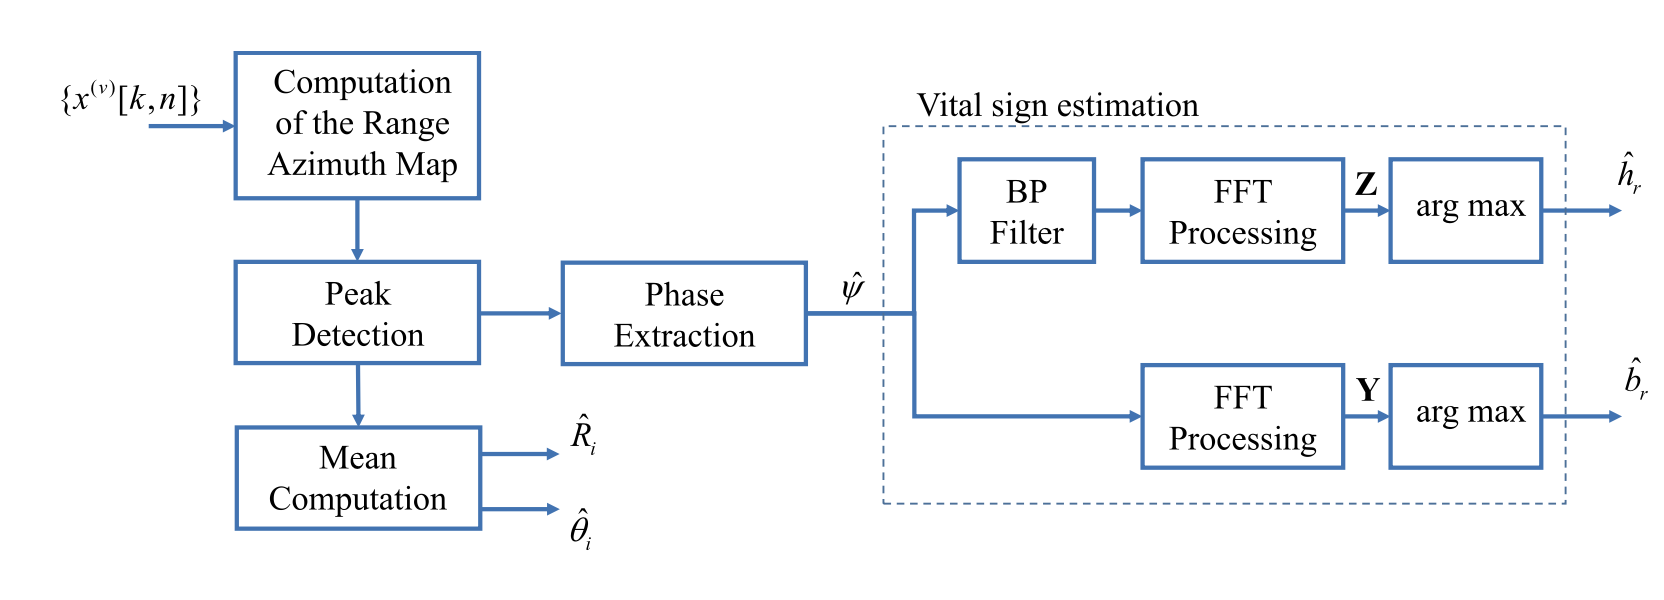
\includegraphics[width=0.7\linewidth]{Images/chapter3/3-3.png}
    \caption{
   نمایش پردازش سیگنال علائم حیاتی \lr{(HR و BR)} چندین نفر با استفاده از یک رادار \lr{MIMO} با موقعیت مکانی مشترک.
    \cite{paterniani2023radar}.}
    \label{fig:fmcw_vitals}
\end{figure}


\subsection{استخراج سیگنال میانی (\lr{Beat Signal}) و کالیبراسیون \lr{DC}}
\label{sec:beat-signal-dc-calibration}

پس از دریافت داده‌های \lr{IF} از مبدل آنالوگ‌به‌دیجیتال، یک \lr{FFT} مختصر (\lr{Slow-Time FFT}) روی هر چیپ انجام می‌شود تا فرکانس مناسب (\lr{bin}) مربوط به بازتاب از قفسه‌ی سینه انتخاب گردد. سپس سیگنال‌های \lr{I/Q} متناظر با آن \lr{bin} برای مراحل بعدی استخراج می‌شود.

از آنجا که خطاهای ساختاری ناشی از عدم تقارن \lr{I/Q} و \lr{DC Offset} می‌تواند موجب انحراف در فاز استخراجی شود، ابتدا با روش \lr{Least-Squares Circle Fitting} مؤلفه‌های \lr{DC} مجزای \lr{I} و \lr{Q} برآورد و حذف می‌شوند. با این کار، شکل موج فازِ استخراج‌شده به بازتاب واقعی سیگنال ضربان قلب نزدیک‌تر می‌گردد.


\subsection{استخراج فاز و آشفتگی‌زدایی (\lr{Phase Unwrapping})}
\label{sec:phase-unwrapping}

برای به‌دست آوردن فاز پیوسته‌ی حرکت قفسه‌ی سینه، از تابع آرکتانژانت دو متغیره استفاده می‌شود:

\begin{equation}
\phi[n] = \operatorname{atan2}(Q[n],\, I[n])
\label{eq:phase_extraction}
\end{equation}
\addequation{استخراج فاز از مؤلفه‌های \lr{I} و \lr{Q} با تابع آرکتانژانت دوارگشتی}

که خروجی در بازه $-\pi$ تا $\pi$ قرار دارد. سپس برای حذف جهش‌های ناخواسته بزرگ‌تر از $\pi$، الگوریتم \lr{Unwrapping} اجرا می‌شود. برای مواردی که جابجایی دیواره بیش از نیم طول موج باشد و \lr{Unwrapping} ساده خطا دهد، می‌توان از الگوریتم \lr{DACM (Differencing and Augmented Cross-Multiplication)} بهره برد.

\subsection{تقویت اجزاء ضربان قلب و حذف درفت فاز}
\label{sec:phase-detrend}

در سیگنال \lr{Unwrapped Phase}، مؤلفه‌های تنفسی با بازه‌ی فرکانسی بین 0.1 تا 0.5~\lr{Hz} معمولاً غالب‌تر از مؤلفه‌های ضربان قلب در بازه‌ی 0.8 تا 2.0~\lr{Hz} هستند. برای تقویت مؤلفه‌های ضربان، ابتدا تفاضل مرکزی فاز (بین نمونه‌های جلو و عقب) محاسبه می‌شود تا شیب‌های لحظه‌ای برجسته شوند:

\begin{equation}
\Delta \phi[n] = \phi[n+1] - \phi[n-1]
\label{eq:phase_diff}
\end{equation}
\addequation{محاسبه تفاضل مرکزی برای حذف روند و تقویت مولفه‌های پرنوسان مانند ضربان قلب}

در مواردی که مقدار تفاضل از آستانه‌ای بیش از حد بزرگ یا کوچک‌تر از منفی آستانه باشد، نمونه‌ها با درون‌یابی خطی اصلاح می‌شوند تا ناهمواری‌های ضربه‌ای (\lr{Impulse Noise}) برطرف گردد.

\subsection{فیلترینگ ناظر بر جداسازی بلوک‌های تنفس و ضربان}
\label{sec:bandpass-filtering}

پس از تفاضل فاز، دو فیلتر \lr{Bandpass IIR} مجزا اعمال می‌شود:

\begin{itemize}
  \item \lr{فیلتر دومرحله‌ای}: برای تفکیک مؤلفه‌های تنفسی در بازه‌ی فرکانسی \lr{0.1–0.5 Hz}
  \item \lr{فیلتر چهارمرحله‌ای}: برای جداسازی ضربان قلب در بازه‌ی \lr{0.8–2.0 Hz}
\end{itemize}

این ساختار به شکل بلادرنگ روی سیگنال اعمال و خروجی هر فیلتر برای مراحل بعدی نگهداری می‌شود.

\subsection{حذف اعوجاج ناشی از حرکت و کنترل بهره}
\label{sec:motion-artifacts}

برای مقابله با تداخل ناشی از حرکت‌های بزرگ بدن (\lr{Motion Corruption})، انرژی هر بخش یک‌ثانیه‌ای سیگنال ضربان قلب محاسبه می‌شود و با آستانه‌ای مقایسه می‌گردد:

\begin{equation}
E = \sum_{n=1}^{N} x^2[n]
\label{eq:energy}
\end{equation}
\addequation{محاسبه انرژی سیگنال در یک بازه زمانی به‌منظور شناسایی حرکت‌های ناخواسته}

در صورت عبور از آستانه، سیگنال مقیاس شده یا حذف می‌شود تا از ورود نویزهای حرکتی به تخمین جلوگیری گردد.

\subsection{ شناسایی پیک طیفی برای تخمین ضربان قلب}
\label{sec:peak-counting}

برای استخراج \lr{HR}، یک \lr{FFT} روی بخش‌های سالم خروجی فیلتر ضربان اجرا شده و قله‌ی طیفی متناظر با فرکانس قلب شناسایی می‌شود. تعداد پیک‌های متوالی در بازه‌ی زمانی مشخص، معادل نرخ ضربان قلب بر حسب \lr{bpm} است.

\subsection{تحلیل زمان فرکانس (\lr{STFT})}
\label{sec:stft}

به‌منظور ردیابی تغییرات لحظه‌ای ضربان و جداسازی بهتر هارمونیک‌های تنفس، از روش \lr{Short-Time Fourier Transform (STFT)} استفاده می‌شود. در هر پنجره‌ی زمانی، انرژی ترکیبی سیگنال به‌صورت زیر محاسبه می‌گردد:

\begin{equation}
E[n] = |x[n]|^2 + |y[n]|^2
\label{eq:stft_energy}
\end{equation}
\addequation{محاسبه انرژی در تحلیل \lr{STFT} برای تشخیص بازتاب‌های قوی از سطح بدن}

نقاط با بیشترین انرژی، بازتاب‌های ضربان قلب تلقی شده و تحلیل ادامه می‌یابد.

\subsection{الگوریتم \lr{Health-VMD} برای استخراج دقیق \lr{HRV}}
\label{sec:health-vmd}

برای تخمین \lr{HRV} نیاز به تشخیص دقیق هر ضربان (\lr{IBI}) است. در مقاله‌ی \lr{Health-Radar}، روش \lr{Variational Mode Decomposition (VMD)} با پارامترهای بهینه‌سازی‌شده توسط الگوریتم \lr{GOA (Grasshopper Optimization Algorithm)} پیشنهاد شده است. تابع هدف پیشنهادی:

\begin{equation}
\mathrm{PME} = \alpha \cdot H_{\mathrm{PE}} + \beta \cdot I_{\mathrm{MI}} + \gamma \cdot L_{\mathrm{Loss}}
\label{eq:pme_objective}
\end{equation}
\addequation{تابع هدف ترکیبی برای \lr{VMD} شامل آنتروپی جایگشتی، اطلاعات متقابل و نرخ اتلاف انرژی}


این روش تضمین می‌کند که هارمونیک‌های تنفس وارد مدهای ضربان نشوند. خروجی این الگوریتم، تخمین دقیق پارامترهایی نظیر \lr{SDNN} و \lr{RMSSD} است، با دقتی برابر:

\begin{equation}
\mathrm{RMSE} \approx 4.1\ \mathrm{ms}
\label{eq:rmse_sdnn}
\end{equation}
\addequation{خطای میانگین مربعی در تخمین \lr{SDNN} توسط الگوریتم \lr{Health-VMD}}

\subsection*{خلاصه‌ی نتایج}
\label{sec:summary}

با ترکیب مراحل فوق کالیبراسیون \lr{DC}، استخراج و \lr{Unwrapping} فاز، تفاضل و فیلترینگ \lr{IIR}، حذف آرتیفکت‌های حرکتی، \lr{STFT} و \lr{Health-VMD} دقت تخمین \lr{HR} به‌صورت زیر گزارش شده است:

\begin{equation}
\mathrm{MAE} < 2\ \mathrm{bpm},\quad \mathrm{RMSE_{HRV}} \approx 5\ \mathrm{ms}
\label{eq:hr_final_results}
\end{equation}
\addequation{دقت نهایی زنجیره‌ی پردازش در تخمین \lr{HR} و \lr{HRV} در شرایط بالینی}


% ====================  ملاحظات ایمنی و استانداردها  ====================
\section{ملاحظات ایمنی و انطباق با استانداردهای پزشکی}
\label{sec:safety-standards}

در طراحی و پیاده‌سازی رادارهای \lr{FMCW} برای کاربردهای پزشکی غیرتماسی، رعایت استانداردهای ایمنی تابش الکترومغناطیسی و الزامات بالینی از اهمیت بالایی برخوردار است. این فصل به بررسی محدودیت‌های توان خروجی، معیارهای تشعشع و تداخل الکترومغناطیسی، و مستندات فنی مرتبط با تجهیزات پزشکی می‌پردازد.

\subsection{محدودیت توان خروجی و تابش سطحی}
\label{sec:power-density-limits}

طبق راهنمای \lr{ICNIRP} (کمیسیون بین‌المللی حفاظت در برابر تشعشع غیر‌یونیزه) و مقررات \lr{FCC} در ایالات متحده، میزان چگالی توان مجاز برای فرکانس‌های میلی‌متری‌موج در محدوده‌ی \lr{30–300 GHz} نباید از \lr{10 W/m²} در برخورد پوستی فراتر رود.

در سامانه‌های مبتنی بر چیپ‌های \lr{BGT} و \lr{IWR1642}، توان خروجی تنظیم‌شده حدود \lr{5 dBm} ($\sim$\lr{3.16 mW}) است که با توجه به آنتن‌های با بهره‌ی \lr{3–4 dBi} و فاصله‌ی عملیاتی \lr{0.5–3} متر، چگالی توان در سطح بدن فراتر از \lr{0.1 W/m²} نخواهد رفت. این مقدار به‌طور ایمن زیر حد \lr{ICNIRP} و \lr{FCC} قرار دارد و مطابق با توصیه‌های \lr{EPA} نیز ریسک زیستی محسوب نمی‌شود.

\subsection{معیارهای تشعشع الکترومغناطیسی و تداخل}
\label{sec:emc-sar}

برای حصول اطمینان از عدم تداخل با تجهیزات پزشکی حساس در بیمارستان‌ها (مثل مونیتورهای \lr{ECG} و پمپ‌های تزریق)، استانداردهای \lr{IEC 60601-1-2:2014} برای سازگاری الکترومغناطیسی (\lr{EMC}) باید رعایت شوند. این استاندارد مشخص می‌کند که دستگاه نباید میدان‌های ناخواسته با فرکانس‌های ناهمگن تولید کند و باید در برابر اختلالات محیطی تا سطح مشخص‌شده مقاوم باشد.

همچنین، استاندارد \lr{IEEE 1528:202X} (اصلاح‌شده برای رادارهای \lr{mmWave}) روش آزمون تابش را برای دستگاه‌های بردکوتاه پزشکی تعریف می‌کند. بر اساس آن، اندازه‌گیری \lr{SAR} (نرخ جذب ویژه) برای هر نقطه باید کمتر از \lr{2 W/kg} در بازه‌ی \lr{10} گرم بافت باشد. شبیه‌سازی‌های پراکندگی پرتو نشان داده‌اند که با توان خروجی \lr{5 dBm} و فاصله بیش از \lr{20} سانتی‌متر، \lr{SAR} به حدود \lr{0.05 W/kg} می‌رسد که به‌طور قابل‌توجهی زیر حد مجاز است.

\subsection{ایمنی بیماران و اپراتورها}
\label{sec:patient-operator-safety}

علاوه بر محیط بیمارستان، در کاربردهای بیمار در منزل نیز باید الزامات سادگی کاربری و هشدار خطر رعایت شود. طبق \lr{ISO 14971:2019} برای مدیریت خطر در تجهیزات پزشکی، باید ریسک‌های بالقوه ناشی از تابش الکترومغناطیسی، تداخل الکتریکی و ایمنی الکتریکی (\lr{IEC 60601-1:2005}) مستندسازی و تحلیل شوند.

\begin{itemize}
  \item \textbf{تابش امواج:} با توجه به توان پایین و ساختار بسته آنتن‌ها، خطر مستقیم تابش کاهش یافته است.
  \item \textbf{اختلال الکتریکی:} با قرار دادن فیلترهای \lr{EMI} و فریت‌بیرینگ روی خطوط تغذیه و سیگنال، پایداری الکترومغناطیسی حفظ می‌شود.
  \item \textbf{ایمنی برق:} رعایت استانداردهای حفاظت در برابر شوک الکتریکی (\lr{IEC 60601-1}) و استفاده از مدارهای جداساز (\lr{Isolator}) در بخش تغذیه \lr{USB} اطمینان می‌دهد که هیچ تماس مستقیم کاربر با سطوح ولتاژ بالا رخ ندهد.
\end{itemize}

\subsection{فرایند صدور گواهی و ثبت بالینی}
\label{sec:certification-process}

برای ورود به بازار تجهیزات پزشکی، دستگاه باید در چارچوب \lr{FDA} (ایالات متحده)، \lr{CE} (اروپا) و \lr{IR-MOH} (ایران) ثبت شود. مراحل اصلی عبارت‌اند از:

\begin{enumerate}
  \item \textbf{وثیقه‌نگاری فنی:} شامل گزارشات طراحی، آزمون \lr{EMC}، \lr{SAR} و تحلیل ریسک (\lr{ISO 14971}).
  \item \textbf{آزمون‌های کارآزمایی بالینی:} مطابق با \lr{ISO 14155}، باید مطالعه‌ای کنترل‌شده با حداقل ۲۰ بیمار انجام گیرد تا دقت و ایمنی دستگاه تأیید شود.
  \item \textbf{تهیه مستندات کیفی:} \lr{Quality Management System} مطابق \lr{ISO 13485} برای تضمین سازگاری تولید.
\end{enumerate}

این فرایندها معمولاً \lr{12–18} ماه زمان می‌برند اما برای سامانه‌های کم‌خطر (\lr{Class IIa} در اروپا) مسیر تسهیل‌شده (\lr{MDR}) وجود دارد که زمان ثبت را به حدود \lr{9} ماه کاهش می‌دهد.

\subsection*{جمع‌بندی بخش}
\label{sec:safety-summary}

با تنظیم توان خروجی پایین، طراحی مطابق با استانداردهای \lr{EMC} و \lr{SAR}، و مستندسازی فرایندهای مدیریت ریسک و ثبت بالینی، سامانه راداری موردنظر الزامات ایمنی و قانونی برای استفاده در محیط‌های بالینی و خانگی را تأمین می‌نماید.


% ====================  نتایج  ====================
\section{جمع‌بندی و نتیجه‌گیری}
\label{sec:conclusion}

در این پایان‌نامه، طراحی و پیاده‌سازی سامانه‌های غیرتماسی پایش علائم حیاتی مبتنی بر رادار \lr{FMCW} بررسی شد. مهم‌ترین نتایج به‌صورت زیر خلاصه می‌شوند:

\begin{enumerate}
    \item \textbf{تعیین برتری معماری \lr{FMCW}:}
    \begin{itemize}
        \item رادارهای \lr{FMCW} توازن مناسبی بین پیچیدگی سخت‌افزاری و قابلیت‌های فاصله‌یابی و تفکیک چندهدفه ارائه می‌دهند، در حالی که \lr{CW} از نظر سخت‌افزار ساده بوده اما در برابر کلاتر محیطی آسیب‌پذیر است و \lr{UWB} با وجود دقت بالا نیازمند سخت‌افزار و پردازش پیشرفته است.
        \item تحلیل داده‌های تجربی نشان داد که معماری \lr{FMCW} پایین‌ترین میانه‌ی خطای مطلق ($\mathrm{MAE} < 2\ \mathrm{bpm}$) در اندازه‌گیری ضربان قلب را ثبت کرده است و توزیع خطاهای آن فشرده‌تر از دو معماری دیگر است.
    \end{itemize}

    \item \textbf{انتخاب بهینه فرکانس و پهنای باند:}
    \begin{itemize}
        \item پهنای باند در محدوده‌ی \lr{1–4 GHz}، رزولوشن فاصله‌ای زیرسانتی‌متری را برای کاربردهای پزشکی در برد عملیاتی \lr{0.5–3 m} فراهم می‌کند.
        \item فرکانس‌های حامل میانی (\lr{60–80 GHz}) به دلیل حساسیت فاز مناسب و عمق نفوذ کافی، بهترین گزینه برای سامانه‌های پوشیدنی و بالینی هستند؛ فرکانس‌های بالاتر تا \lr{120 GHz} دقت بیشتری ارائه می‌دهند اما پیچیدگی آنتن و مصرف انرژی را افزایش می‌دهند.
    \end{itemize}

    \item \textbf{معماری سخت‌افزار و \lr{MIMO}:}
    \begin{itemize}
        \item استفاده از چیپ \lr{IWR1642} با آرایه \lr{MIMO} (۳\lr{TX}$\times$۴\lr{RX}) امکان جداسازی چندشخصه و تعیین زاویه را به‌سادگی فراهم می‌کند و وضوح زاویه‌ای حدود $16.6^\circ \times 45^\circ$ را میسر می‌سازد.
        \item بردهای ارزیابی ماژولار مبتنی بر \lr{BGT24} و \lr{BGT60} امکان مقایسه و تنظیم سریع پارامترها را فراهم می‌کنند و مصرف توان سیستم نهایی زیر \lr{30 mW} حفظ شده است.
    \end{itemize}

    \item \textbf{الگوریتم‌های پردازش سیگنال:}
    \begin{itemize}
        \item زنجیره‌ی پردازش شامل کالیبراسیون \lr{DC}، استخراج و \lr{Unwrapping} فاز، تفاضل فاز و فیلترینگ \lr{IIR}، حذف آرتیفکت حرکتی و \lr{STFT} است که دقت \lr{HR} را تا $\mathrm{MAE} < 2\ \mathrm{bpm}$ تضمین می‌کند.
        \item الگوریتم \lr{Health-VMD} با تابع هدف \lr{PME} و بهینه‌سازی \lr{GOA} امکان استخراج دقیق \lr{HRV} با $\mathrm{RMSE} \approx 4.1\ \mathrm{ms}$ را مهیا ساخته است، که در کاربردهای چندنفری عملکرد پایدار دارد.
    \end{itemize}

    \item \textbf{رعایت ایمنی و استانداردها:}
    \begin{itemize}
        \item توان خروجی تنظیم‌شده ($\sim$3.16 \lr{mW}) به‌طور ایمن زیر محدودیت‌های \lr{ICNIRP} و \lr{FCC} قرار دارد و \lr{SAR} کمتر از \lr{0.05 W/kg} است.
        \item انطباق با استانداردهای \lr{IEC 60601-1-2}، \lr{IEEE 1528} و \lr{ISO 14971} فرایند ثبت \lr{FDA}، \lr{CE} و \lr{IR-MOH} را تسهیل می‌کند و خطرات تابش و تداخل به حداقل می‌رسد.
    \end{itemize}
\end{enumerate}

\subsection*{چشم‌انداز آینده}
\label{sec:future-work}

با وجود پیشرفت‌های قابل توجه در سامانه‌های \lr{FMCW} پزشکی، فرصت‌های پژوهشی متعددی باقی است:

\begin{itemize}
    \item \textbf{هوش مصنوعی در پردازش بلادرنگ:} ترکیب یادگیری عمیق با مراحل پردازش می‌تواند دقت و مقاومت الگوریتم‌ها در برابر حرکت‌های تصادفی را بهبود بخشد.
    \item \textbf{بهینه‌سازی انرژی و طراحی پوشیدنی:} تحقیق روی منابع انرژی کم‌حجم و ادغام سامانه در پوشیدنی‌های سبک (مانند ساعت هوشمند) برای نظارت مداوم بی‌وقفه.
    \item \textbf{گسترش به علائم حیاتی دیگر:} توسعه الگوریتم‌های تحلیل سیگنال برای اندازه‌گیری فشار خون، اشباع اکسیژن و دمای پوست با استفاده از ترکیب چندحسی.
    \item \textbf{مطالعات بالینی گسترده:} اجرای آزمون‌های چندمرکزه با جمعیت متنوع برای اعتبارسنجی نتایج در محیط‌های بالینی واقعی.
\end{itemize}

در نهایت، سامانه‌های \lr{FMCW} با پتانسیل تطبیق‌پذیری بالا و قابلیت ترکیب با فناوری‌های پوشیدنی، افق روشنی برای پزشکی از راه دور و مراقبت‌های هوشمند باز می‌کنند. این پایان‌نامه با ارائه یک چارچوب یکپارچه از مبانی تئوری تا پیاده‌سازی عملی، گامی مهم در جهت توسعه این فناوری برداشته است.




% You would typically have your \title, \author, \maketitle, \tableofcontents here.
% Assuming this chapter follows Chapter 3.

\chapter{پردازش سیگنال، آزمایش‌ها و نتایج} % Chapter 4
\label{ch:signal-processing-experiments-results}

\section{روش‌‌های پردازش فاز و دامنه} % Section 4.1
\label{sec:phase-amplitude-processing}

\subsection{دمدولاسیون فازی} % Subsection 4.1.1
\label{sec:phase-demodulation}
% Add your text content for this subsection here.

\subsection{جداسازی باند ضربان و تنفس} % Subsection 4.1.2
\label{sec:heart-breath-band-separation}
% Add your text content for this subsection here.

\section{الگوریتم‌‌های تحلیلی} % Section 4.2
\label{sec:analytical-algorithms}

\subsection{\lr{FFT} و \lr{STFT}} % Subsection 4.2.1
\label{sec:fft-stft}
% Add your text content for this subsection here.

\subsection{\lr{Wavelet} و مدل‌سازی \lr{AR}} % Subsection 4.2.2
\label{sec:wavelet-ar-modeling}
% Add your text content for this subsection here.

\section{طراحی آزمایش و پروتکل} % Section 4.3
\label{sec:experiment-design-protocol}

\subsection{تجهیزات مرجع (\lr{ECG} / پالس اکسیمتر)} % Subsection 4.3.1
\label{sec:reference-equipment}
% Add your text content for this subsection here.

\subsection{نحوه قرارگیری سوژه و سناریوها} % Subsection 4.3.2
\label{sec:subject-placement-scenarios}
% Add your text content for this subsection here.

\section{نتایج تجربی} % Section 4.4
\label{sec:experimental-results}

\subsection{مقایسه با مرجع} % Subsection 4.4.1
\label{sec:comparison-with-reference}
% Add your text content for this subsection here.

\subsection{تحلیل خطا و منابع نویز} % Subsection 4.4.2
\label{sec:error-noise-analysis}
% Add your text content for this subsection here.

\section{بحث و تفسیر نتایج} % Section 4.5
\label{sec:discussion-interpretation}
% Add your text content for this section here.

% You would typically have your \title, \author, \maketitle, \tableofcontents here.
% Assuming this chapter follows Chapter 4.

\chapter{نتیجه‌گیری و پیشنهادات} % Chapter 5
\label{ch:conclusion-suggestions}

\section{خلاصه دستاوردهای پژوهش} % Section 5.1
\label{sec:research-achievements-summary}
% Add your text content for this section here.

\section{پاسخ به سوالات و اهداف} % Section 5.2
\label{sec:answers-to-questions-goals}
% Add your text content for this section here.

\section{محدودیت‌ها} % Section 5.3
\label{sec:limitations}
% Add your text content for this section here.

\section{پیشنهادات برای پژوهش‌های آتی} % Section 5.4
\label{sec:future-research-suggestions}
% Add your text content for this section here.

\section{کاربردهای عملی و چشم‌انداز} % Section 5.5
\label{sec:practical-applications-outlook}
% Add your text content for this section here.
\chapter{موارد به‌روزرسانی}



%--------------------------------------------------------------------------appendix( مراجع و پیوست ها)
\chapterfont{\vspace*{-2em}\centering\LARGE}%

\appendix
\bibliographystyle{unsrt-fa}
\bibliography{references}
\chapter*{‌پیوست}
\markboth{پیوست}{}
\addcontentsline{toc}{chapter}{پیوست}
موضوعات مرتبط با متن گزارش پایان نامه كه در يكی از گروه‌های زير قرار می‌گيرد، در بخش پيوست‌ها آورده شوند:
\begin{enumerate}
\item  اثبات های رياضی يا عمليات رياضی طولانی‌.‌
\item داده و اطلاعات نمونه (های) مورد مطالعه (\lr{Case Study}) چنانچه طولانی باشد‌.‌
\item نتايج كارهای ديگران چنانچه نياز به تفصيل باشد‌.‌
\item مجموعه تعاريف متغيرها و پارامترها، چنانچه طولانی بوده و در متن به انجام نرسيده باشد‌.‌
\end{enumerate}
% براي شماره‌گذاري روابط، جداول و اشكال موجود در پيوست‌ از ساختار متفاوتي نسبت به متن اصلي استفاده مي‌شود كه در زير به‌عنوان نمونه نمايش داده شده‌است. 
% \begin{equation}
%F=ma
%\end{equation}
\section*{کد میپل }
\begin{latin}
\begin{verbatim}

with(DifferentialGeometry):
with(Tensor):
DGsetup([x, y, z], M)
																	frame name: M
a := evalDG(D_x)
																	D_x
b := evalDG(-2 y z D_x+2 x D_y/z^3-D_z/z^2)


\end{verbatim}
\end{latin}
%--------------------------------------------------------------------------dictionary(واژه نامه ها)
%اگر مایل به داشتن صفحه واژه‌نامه نیستید، خط زیر را غیر فعال کنید.
\parindent=0pt
%
\chapter*{واژه‌نامه‌ی فارسی به انگلیسی}
\pagestyle{style9}

\addcontentsline{toc}{chapter}{واژه‌نامه‌ی فارسی به انگلیسی}
%%%%%%
\begin{multicols*}{2}

{\bf آ}
\vspace*{3mm}


\farsiTOenglish{اسکالر}{Scalar}


\vspace*{3mm}
{\bf ب}
\vspace*{3mm}

\farsiTOenglish{بالابر}{Lift}


\vspace*{3mm}
{\bf پ}
%%\vspace*{3mm}

\farsiTOenglish{پایا}{Invariant}



\vspace*{3mm}
{\bf ت}
%%\vspace*{3mm}

\farsiTOenglish{ تناظر }{Correspondence}


\vspace*{3mm}
{\bf ث}
%%\vspace*{3mm}

\farsiTOenglish{ثابت‌ساز}{Stabilizer}

\vspace*{3mm}
{\bf ج}
%%\vspace*{3mm}

\farsiTOenglish{جایگشت}{Permutation}



\vspace*{3mm}
{\bf چ}
%%\vspace*{3mm}


\farsiTOenglish{چند جمله‌ای }{Polynomial}

\vspace*{3mm}
{\bf ح}
%%\vspace*{3mm}

\farsiTOenglish{حاصل‌ضرب دکارتی}{Cartesian product}


\vspace*{3mm}
{\bf خ}
%%\vspace*{3mm}

\farsiTOenglish{خودریختی}{Automorphism}

\vspace*{3mm}
{\bf د}
%%\vspace*{3mm}

\farsiTOenglish{درجه}{Degree}


\vspace*{3mm}
{\bf ر}
%%\vspace*{3mm}


\farsiTOenglish{ریزپردازنده}{microprocessor}


\vspace*{3mm}
{\bf ز}
%%\vspace*{3mm}


\farsiTOenglish{زیرمدول}{Submodule}


\vspace*{3mm}
{\bf س}
%%\vspace*{3mm}

\farsiTOenglish{سرشت}{Character}


\vspace*{3mm}
{\bf ص}
%%\vspace*{3mm}

\farsiTOenglish{صادقانه}{Faithful}

\vspace*{3mm}
{\bf ض}
%%\vspace*{3mm}

\farsiTOenglish{ضرب داخلی}{Inner product}

\vspace*{3mm}
{\bf ط}
%%\vspace*{3mm}


\farsiTOenglish{طوقه}{Loop}


\vspace*{3mm}
{\bf ظ}
%%\vspace*{3mm}


\farsiTOenglish{ظرفیت}{Valency}
 
\vspace*{3mm}
{\bf ع}
%%\vspace*{3mm}


\farsiTOenglish{عدم مجاورت}{Nonadjacency}



\vspace*{3mm}
{\bf ف}
%%\vspace*{3mm}

\farsiTOenglish{فضای برداری}{Vector space}



\vspace*{3mm}
{\bf ک}
%%\vspace*{3mm}

\farsiTOenglish{کاملاً تحویل‌پذیر}{Complete reducibility}


\vspace*{3mm}
{\bf گ}
%%\vspace*{3mm}


\farsiTOenglish{گراف}{Graph}



\vspace*{3mm}
{\bf م}
%%\vspace*{3mm}

\farsiTOenglish{ماتریس جایگشتی}{Permutation matrix }


\vspace*{3mm}
{\bf ن}
%%\vspace*{3mm}

\farsiTOenglish{ناهمبند}{Disconnected}


\vspace*{3mm}
{\bf و}
%%\vspace*{3mm}

\farsiTOenglish{وارون‌پذیر}{Invertible}


\vspace*{3mm}
{\bf ه}
%%\vspace*{3mm}

\farsiTOenglish{همبند}{Connected}



\vspace*{3mm}
{\bf ی}
%%\vspace*{3mm}

\farsiTOenglish{یال}{Edge}




\end{multicols*}%
\chapter*{واژه‌نامه انگلیسی به فارسی}
\pagestyle{style9}
\addcontentsline{toc}{chapter}{واژه‌نامه انگلیسی به فارسی}

\begin{longtable}{|p{7cm}|p{7cm}|}
\caption[]{واژه‌نامه انگلیسی به فارسی}\\
\hline
\textbf{واژه انگلیسی} & \textbf{معادل فارسی} \\
\hline
\endfirsthead
\multicolumn{2}{c}%
{{\tablename\ \thetable{}   ادامه واژه‌نامه از صفحه قبل}} \\
\hline
\textbf{واژه انگلیسی} & \textbf{معادل فارسی} \\
\hline
\endhead
\hline \multicolumn{2}{r}{{ادامه در صفحه بعد}} \\ 
\endfoot
\hline
\endlastfoot

\lr{antenna} & آنتن \\
\hline
\lr{radar antenna} & \lr{رادار} آنتن \\
\hline
\lr{algorithm} & الگوریتم \\
\hline
\lr{advanced signal processing algorithms} & الگوریتم‌های پیشرفته پردازش سیگنال \\
\hline
\lr{heart rate extraction algorithms} & الگوریتم‌های استخراج نرخ ضربان قلب \\
\hline
\lr{myocardial expansion} & انبساط میوکارد \\
\hline
\lr{myocardial contraction} & انقباض میوکارد \\
\hline
\lr{pulse oximeter} & اکسی‌متر پالس \\
\hline
\lr{range detection} & آشکارسازی فاصله \\
\hline
\lr{velocity detection} & آشکارسازی سرعت \\
\hline
\lr{radar chipset selection} & انتخاب چیپ‌ست رادار \\
\hline
\lr{frequency selection} & انتخاب فرکانس \\
\hline
\lr{perfusion data} & اطالاعات پرفیوژن \\
\hline
\lr{evaluation board} & برد ارزیابی \\
\hline
\lr{detection range} & برد آشکار \\
\hline
\lr{Fourier transform} & تبدیلات (تبدیل فوریه) \\
\hline
\lr{wavelet transform} & تبدیل ویولت \\
\hline
\lr{transmitted power} & توان ارسالی \\
\hline
\lr{chirp signal} & تحریک سیگنال چیپ \\
\hline
\lr{singular value decomposition (SVD)} & تجزیه مقادیر منفرد (\lr{SVD}) \\
\hline
\lr{trade-off} & تخصیص (\lr{trade-off}) \\
\hline
\lr{hardware design} & طراحی سخت‌افزار \\
\hline
\lr{system design} & طراحی سیستم \\
\hline
\lr{physical obstacles} & تعریف موانع فیزیکی \\
\hline
\lr{Doppler velocity} & سرعت داپلر \\
\hline
\lr{speed of light (c)} & سرعت نور (\lr{c}) \\
\hline
\lr{reflected signal} & سیگنال برگشتی \\
\hline
\lr{radar signal} & سیگنال رادار \\
\hline
\lr{chirp signal} & سیگنال چیپ \\
\hline
\lr{seismocardiogram} & سیزموکاردیوگرام \\
\hline
\lr{phase drift removal} & شکاف درفت فاز (\lr{phase drift removal}) \\
\hline
\lr{field of view} & شعاع میدان دید \\
\hline
\lr{spectral peak identification} & شناسایی پیک طیفی \\
\hline
\lr{implementation} & پیاده‌سازی \\
\hline
\lr{penetration depth} & عمیق نفوذ \\
\hline
\lr{non-contact} & غیرتماسی \\
\hline
\lr{non-invasive} & غیرتهاجمی \\
\hline
\lr{adaptive filtering} & فیلتر تطبیقی \\
\hline
\lr{digital filter} & فیلتر دیجیتال \\
\hline
\lr{filtering} & فیلترینگ \\
\hline
\lr{beat frequency (fb)} & فرکانس بیت (\lr{fb}) \\
\hline
\lr{carrier frequency (fc)} & فرکانس حامل (\lr{fc}) \\
\hline
\lr{physiology of heartbeat} & فیزیولوژی ضربان قلب \\
\hline
\lr{data processing} & فشرده‌سازی داده (پردازش داده) \\
\hline
\lr{cluttered environment} & ظرفیت محیط شلوغ \\
\hline
\lr{electromagnetic emission criteria} & معیار تشعشع الکترومغناطیسی \\
\hline
\lr{safety considerations} & ملاحظات ایمنی \\
\hline
\lr{mean absolute error (MAE)} & میانگین قدر مطلق خطا (\lr{MAE}) \\
\hline
\lr{phase sensitivity} & میزان حساسیت فاز \\
\hline
\lr{advantages and limitations} & مزایا و محدودیت‌ها \\
\hline
\lr{environmental clutter} & مزاحمت محیطی \\
\hline
\lr{stability / robustness} & مقاوم‌سازی (پایداری) \\
\hline
\lr{trade-off} & موازنه \\
\hline
\lr{medical standards} & مهندسی استانداردهای پزشکی \\
\hline
\lr{remote monitoring} & نظارت از راه دور \\
\hline
\lr{electrocardiogram (ECG)} & نوسان‌سنج (\lr{ECG}) \\
\hline
\lr{advanced signal processing algorithms} & نرم‌افزارهای پردازش سیگنال \\
\hline
\lr{principles of operation} & نکات کلیدی طراحی رادار \\
\hline
\lr{principles of operation} & نکات کلیدی طراحی رادار \lr{FMCW} \\
\hline
\lr{principles of operation} & نکات کلیدی طراحی رادار \lr{UWB} \\
\hline
\lr{principles of operation} & نکات کلیدی طراحی رادار \lr{CW} \\
\hline
\lr{medical monitoring} & ناظر پزشکی \\
\hline
\lr{modular structure} & هسته برداری \\
\hline
\lr{reflected signal} & هجمه (\lr{سیگنال برگشتی}) \\
\hline
\lr{heart rate monitoring} & فشار سنج ضربان قلب \\
\hline
\lr{heart rate} & ضربان قلب \\
\hline
\lr{implementation} & پیاده‌سازی \\
\hline
\lr{field of view} & میدان دید \\
\hline
\lr{FMCW radar} & موج پیوسته مدوله‌شده فرکانسی (\lr{رادار FMCW}) \\
\hline
\lr{CW radar} & موج پیوسته (\lr{رادار CW}) \\
\hline
\lr{chirp} & موج مدولاسیون خطی فرکانسی (چیپ) \\
\hline
\lr{UWB radar} & موج پهن—وسیع (\lr{رادار UWB}) \\
\hline
\lr{gain control} & \lr{گِین کنترل} \\
\hline
\lr{certification} & گواهینامه پزشکی \\
\hline
\lr{beat signal extraction} & لبه سیگنال (\lr{Beat Signal}) \\
\hline
\lr{analog-to-digital converter (ADC)} & مبدل آنالوگ به دیجیتال (\lr{ADC}) \\
\hline
\lr{evaluation board} & ممیزی ارزیابی \\
\hline
\lr{distance (R)} & مسافت (\lr{R}) \\
\hline
\lr{performance metric for VMD (PME)} & معیار عملکرد در حالت \lr{VMD} (\lr{PME}) \\
\hline
\lr{separation of respiration and heartbeat blocks} & نرم‌افزار جداسازی بلوک‌های تنفس و ضربان \\
\hline
\lr{time–frequency analysis (STFT)} & نرم‌افزار تحلیل زمان—فرکانس (\lr{STFT}) \\
\hline
\lr{heart rate variability (HRV)} & نوسان‌سنج ضربان قلب (\lr{HRV}) \\
\hline
\lr{UWB radar} & طیف فوق‌وسیع (\lr{رادار UWB}) \\
\hline
\lr{analog-to-digital converter (ADC)} & مبدل آنالوگ به دیجیتال \\
\hline
\lr{intermediate frequency (IF)} & مبدل فرکانس میانی (\lr{IF}) \\
\hline
\lr{serial peripheral interface / inter-integrated circuit (SPI/I2C)} & رابط‌های دیجیتال (\lr{SPI/I2C}) \\
\hline
\lr{universal serial bus (USB)} & رابط سریال \lr{USB} \\
\hline
\lr{multiple input multiple output (MIMO)} & سامانه \lr{MIMO} \\
\hline
\lr{time division multiplexing (TDM)} & چندپخشی تقسیم زمانی (\lr{TDM}) \\
\hline
\lr{specific absorption rate (SAR)} & نرخ جذب ویژه (\lr{SAR}) \\
\hline
\lr{electromagnetic compatibility (EMC)} & سازگاری الکترومغناطیسی (\lr{EMC}) \\
\hline
\lr{International Electrotechnical Commission (IEC)} & کمیسیون بین‌المللی الکتروتکنیک (\lr{IEC}) \\
\hline
\lr{Federal Communications Commission (FCC)} & کمیسیون ارتباطات فدرال آمریکا (\lr{FCC}) \\
\hline
\lr{International Commission on Non-Ionizing Radiation Protection (ICNIRP)} & کمیسیون بین‌المللی حفاظت در برابر تشعشعات غیر یونساز (\lr{ICNIRP}) \\
\hline
\lr{Environmental Protection Agency (EPA)} & سازمان حفاظت محیط زیست آمریکا (\lr{EPA}) \\
\hline
\lr{International Organization for Standardization (ISO)} & سازمان بین‌المللی استانداردسازی (\lr{ISO}) \\
\hline
\lr{Conformité Européenne (CE)} & علامت استاندارد اتحادیه اروپا (\lr{CE}) \\
\hline
\lr{Food and Drug Administration (FDA)} & سازمان غذا و داروی آمریکا (\lr{FDA}) \\
\hline
\lr{Iranian Ministry of Health (IR-MOH)} & وزارت بهداشت ایران (\lr{IR-MOH}) \\
\hline
\end{longtable}

%--------------------------------------------------------------------------index(نمایه)
%اگر مایل به داشتن صفحه نمایه نیستید، خط زیر را غیر فعال کنید.
\pagestyle{style7}
\printindex
\pagestyle{style7}
%کلمات کلیدی انگلیسی
\latinkeywords{Write a 3 to 5 KeyWords is essential. Example: AUT, M.Sc., Ph. D,..}
%چکیده انگلیسی

\en-abstract{
This page is accurate translation from Persian abstract into English.
}
%%%%%%%%%%%%%%%%%%%%% کدهای زیر را تغییر ندهید.

\newpage
\thispagestyle{empty}
\begin{latin}
\section*{\LARGE\centering Abstract}

\een-abstract

\vspace*{.5cm}
{\large\textbf{Key Words:}}\par
\vspace*{.5cm}
\elatinkeywords
\end{latin}
% در این فایل، عنوان پایان‌نامه، مشخصات خود و چکیده پایان‌نامه را به انگلیسی، وارد کنید.
%%%%%%%%%%%%%%%%%%%%%%%%%%%%%%%%%%%%
\baselineskip=.6cm
\begin{latin}

\latinfaculty{Electrical Engineering (Electronics and Communication)}


\latintitle{Utilization of FMCW Radars for Medical Applications}


\firstlatinsupervisor{Dr. Shahrooz Asadi}

%\secondlatinsupervisor{Second Supervisor}

% \firstlatinadvisor{Dr. }

%\secondlatinadvisor{Second Advisor}

\latinname{Amirhossein}

\latinsurname{Khalili}

\latinthesisdate{May \& 2025}

\latinvtitle
\end{latin}

\end{document}